\documentclass[twoside]{book}

% Packages required by doxygen
\usepackage{calc}
\usepackage{doxygen}
\usepackage{graphicx}
\usepackage[utf8]{inputenc}
\usepackage{makeidx}
\usepackage{multicol}
\usepackage{multirow}
\usepackage{textcomp}
\usepackage[table]{xcolor}

% Font selection
\usepackage[T1]{fontenc}
\usepackage{mathptmx}
\usepackage[scaled=.90]{helvet}
\usepackage{courier}
\usepackage{amssymb}
\usepackage{sectsty}
\renewcommand{\familydefault}{\sfdefault}
\allsectionsfont{%
  \fontseries{bc}\selectfont%
  \color{darkgray}%
}
\renewcommand{\DoxyLabelFont}{%
  \fontseries{bc}\selectfont%
  \color{darkgray}%
}

% Page & text layout
\usepackage{geometry}
\geometry{%
  a4paper,%
  top=2.5cm,%
  bottom=2.5cm,%
  left=2.5cm,%
  right=2.5cm%
}
\tolerance=750
\hfuzz=15pt
\hbadness=750
\setlength{\emergencystretch}{15pt}
\setlength{\parindent}{0cm}
\setlength{\parskip}{0.2cm}
\makeatletter
\renewcommand{\paragraph}{%
  \@startsection{paragraph}{4}{0ex}{-1.0ex}{1.0ex}{%
    \normalfont\normalsize\bfseries\SS@parafont%
  }%
}
\renewcommand{\subparagraph}{%
  \@startsection{subparagraph}{5}{0ex}{-1.0ex}{1.0ex}{%
    \normalfont\normalsize\bfseries\SS@subparafont%
  }%
}
\makeatother

% Headers & footers
\usepackage{fancyhdr}
\pagestyle{fancyplain}
\fancyhead[LE]{\fancyplain{}{\bfseries\thepage}}
\fancyhead[CE]{\fancyplain{}{}}
\fancyhead[RE]{\fancyplain{}{\bfseries\leftmark}}
\fancyhead[LO]{\fancyplain{}{\bfseries\rightmark}}
\fancyhead[CO]{\fancyplain{}{}}
\fancyhead[RO]{\fancyplain{}{\bfseries\thepage}}
\fancyfoot[LE]{\fancyplain{}{}}
\fancyfoot[CE]{\fancyplain{}{}}
\fancyfoot[RE]{\fancyplain{}{\bfseries\scriptsize Generated on Fri Mar 23 2018 18\-:10\-:59 for Class Scheduler by Doxygen }}
\fancyfoot[LO]{\fancyplain{}{\bfseries\scriptsize Generated on Fri Mar 23 2018 18\-:10\-:59 for Class Scheduler by Doxygen }}
\fancyfoot[CO]{\fancyplain{}{}}
\fancyfoot[RO]{\fancyplain{}{}}
\renewcommand{\footrulewidth}{0.4pt}
\renewcommand{\chaptermark}[1]{%
  \markboth{#1}{}%
}
\renewcommand{\sectionmark}[1]{%
  \markright{\thesection\ #1}%
}

% Indices & bibliography
\usepackage{natbib}
\usepackage[titles]{tocloft}
\setcounter{tocdepth}{3}
\setcounter{secnumdepth}{5}
\makeindex

% Hyperlinks (required, but should be loaded last)
\usepackage{ifpdf}
\ifpdf
  \usepackage[pdftex,pagebackref=true]{hyperref}
\else
  \usepackage[ps2pdf,pagebackref=true]{hyperref}
\fi
\hypersetup{%
  colorlinks=true,%
  linkcolor=blue,%
  citecolor=blue,%
  unicode%
}

% Custom commands
\newcommand{\clearemptydoublepage}{%
  \newpage{\pagestyle{empty}\cleardoublepage}%
}


%===== C O N T E N T S =====

\begin{document}

% Titlepage & ToC
\hypersetup{pageanchor=false}
\pagenumbering{roman}
\begin{titlepage}
\vspace*{7cm}
\begin{center}%
{\Large Class Scheduler \\[1ex]\large 0.\-0.\-1 }\\
\vspace*{1cm}
{\large Generated by Doxygen 1.8.6}\\
\vspace*{0.5cm}
{\small Fri Mar 23 2018 18:10:59}\\
\end{center}
\end{titlepage}
\clearemptydoublepage
\tableofcontents
\clearemptydoublepage
\pagenumbering{arabic}
\hypersetup{pageanchor=true}

%--- Begin generated contents ---
\chapter{\mbox{[}Start Bootstrap\mbox{]}(http\-://startbootstrap.com/) -\/ \mbox{[}S\-B Admin 2\mbox{]}(http\-://startbootstrap.com/template-\/overviews/sb-\/admin-\/2/)}
\label{md__home_travis_build__open-_source-_software-_development_class-scheduler_mysite_faculty_data_t969cd63fba649490953be8fc2cc67ea9}
\hypertarget{md__home_travis_build__open-_source-_software-_development_class-scheduler_mysite_faculty_data_t969cd63fba649490953be8fc2cc67ea9}{}
\href{https://cdnjs.com/libraries/startbootstrap-sb-admin-2}{\tt !\mbox{[}C\-D\-N\-J\-S\mbox{]}(https\-://img.\-shields.\-io/cdnjs/v/startbootstrap-\/sb-\/admin-\/2.\-svg)}

\href{http://startbootstrap.com/template-overviews/sb-admin-2/}{\tt S\-B Admin 2} is an open source, admin dashboard template for \href{http://getbootstrap.com/}{\tt Bootstrap} created by \href{http://startbootstrap.com/}{\tt Start Bootstrap}.

\subsection*{Getting Started}

To begin using this template, choose one of the following options to get started\-:
\begin{DoxyItemize}
\item \href{http://startbootstrap.com/template-overviews/sb-admin-2/}{\tt Download the latest release on Start Bootstrap}
\item Clone the repo\-: {\ttfamily git clone \href{https://github.com/BlackrockDigital/startbootstrap-sb-admin-2.git}{\tt https\-://github.\-com/\-Blackrock\-Digital/startbootstrap-\/sb-\/admin-\/2.\-git}}
\item Fork the repo
\end{DoxyItemize}

\subsection*{Using the Source Files}

After cloning the repo take a look at the {\ttfamily gulpfile.\-js} and check out the tasks available\-:
\begin{DoxyItemize}
\item {\ttfamily gulp} The default task will compile the L\-E\-S\-S and J\-S into the {\ttfamily dist} directory and minify the output, and it will copy all vendor libraries from {\ttfamily bower\-\_\-components} into the {\ttfamily vendor} directory
\item {\ttfamily gulp dev} The dev task will serve up a local version of the template and will watch the L\-E\-S\-S, J\-S, and H\-T\-M\-L files for changes and reload the browser windo automatically
\end{DoxyItemize}

To update dependencies, run {\ttfamily bower update} and then run {\ttfamily gulp copy} to copy the updated dependencies into the {\ttfamily vendor} directory

\subsection*{Bugs and Issues}

Have a bug or an issue with this template? \href{https://github.com/BlackrockDigital/startbootstrap-sb-admin-2/issues}{\tt Open a new issue} here on Git\-Hub or leave a comment on the \href{http://startbootstrap.com/template-overviews/sb-admin-2/}{\tt template overview page at Start Bootstrap}.

\subsection*{Creator}

Start Bootstrap was created by and is maintained by $\ast$$\ast$\href{http://davidmiller.io/}{\tt David Miller}$\ast$$\ast$, Owner of \href{http://blackrockdigital.io/}{\tt Blackrock Digital}.


\begin{DoxyItemize}
\item \href{https://twitter.com/davidmillerskt}{\tt https\-://twitter.\-com/davidmillerskt}
\item \href{https://github.com/davidtmiller}{\tt https\-://github.\-com/davidtmiller}
\end{DoxyItemize}

Start Bootstrap is based on the \href{http://getbootstrap.com/}{\tt Bootstrap} framework created by \href{https://twitter.com/mdo}{\tt Mark Otto} and \href{https://twitter.com/fat}{\tt Jacob Thorton}.

\subsection*{Copyright and License}

Copyright 2013-\/2018 Blackrock Digital L\-L\-C. Code released under the \href{https://github.com/BlackrockDigital/startbootstrap-sb-admin-2/blob/gh-pages/LICENSE}{\tt M\-I\-T} license. 
\chapter{\mbox{[}Start Bootstrap\mbox{]}(http\-://startbootstrap.com/) -\/ \mbox{[}S\-B Admin 2\mbox{]}(http\-://startbootstrap.com/template-\/overviews/sb-\/admin-\/2/)}
\label{md__home_travis_build__open-_source-_software-_development_class-scheduler_mysite_polls_template6b25d0f788b6aaccddd1af3595bcde07}
\hypertarget{md__home_travis_build__open-_source-_software-_development_class-scheduler_mysite_polls_template6b25d0f788b6aaccddd1af3595bcde07}{}
\href{https://cdnjs.com/libraries/startbootstrap-sb-admin-2}{\tt !\mbox{[}C\-D\-N\-J\-S\mbox{]}(https\-://img.\-shields.\-io/cdnjs/v/startbootstrap-\/sb-\/admin-\/2.\-svg)}

\href{http://startbootstrap.com/template-overviews/sb-admin-2/}{\tt S\-B Admin 2} is an open source, admin dashboard template for \href{http://getbootstrap.com/}{\tt Bootstrap} created by \href{http://startbootstrap.com/}{\tt Start Bootstrap}.

\subsection*{Getting Started}

To begin using this template, choose one of the following options to get started\-:
\begin{DoxyItemize}
\item \href{http://startbootstrap.com/template-overviews/sb-admin-2/}{\tt Download the latest release on Start Bootstrap}
\item Clone the repo\-: {\ttfamily git clone \href{https://github.com/BlackrockDigital/startbootstrap-sb-admin-2.git}{\tt https\-://github.\-com/\-Blackrock\-Digital/startbootstrap-\/sb-\/admin-\/2.\-git}}
\item Fork the repo
\end{DoxyItemize}

\subsection*{Using the Source Files}

After cloning the repo take a look at the {\ttfamily gulpfile.\-js} and check out the tasks available\-:
\begin{DoxyItemize}
\item {\ttfamily gulp} The default task will compile the L\-E\-S\-S and J\-S into the {\ttfamily dist} directory and minify the output, and it will copy all vendor libraries from {\ttfamily bower\-\_\-components} into the {\ttfamily vendor} directory
\item {\ttfamily gulp dev} The dev task will serve up a local version of the template and will watch the L\-E\-S\-S, J\-S, and H\-T\-M\-L files for changes and reload the browser windo automatically
\end{DoxyItemize}

To update dependencies, run {\ttfamily bower update} and then run {\ttfamily gulp copy} to copy the updated dependencies into the {\ttfamily vendor} directory

\subsection*{Bugs and Issues}

Have a bug or an issue with this template? \href{https://github.com/BlackrockDigital/startbootstrap-sb-admin-2/issues}{\tt Open a new issue} here on Git\-Hub or leave a comment on the \href{http://startbootstrap.com/template-overviews/sb-admin-2/}{\tt template overview page at Start Bootstrap}.

\subsection*{Creator}

Start Bootstrap was created by and is maintained by $\ast$$\ast$\href{http://davidmiller.io/}{\tt David Miller}$\ast$$\ast$, Owner of \href{http://blackrockdigital.io/}{\tt Blackrock Digital}.


\begin{DoxyItemize}
\item \href{https://twitter.com/davidmillerskt}{\tt https\-://twitter.\-com/davidmillerskt}
\item \href{https://github.com/davidtmiller}{\tt https\-://github.\-com/davidtmiller}
\end{DoxyItemize}

Start Bootstrap is based on the \href{http://getbootstrap.com/}{\tt Bootstrap} framework created by \href{https://twitter.com/mdo}{\tt Mark Otto} and \href{https://twitter.com/fat}{\tt Jacob Thorton}.

\subsection*{Copyright and License}

Copyright 2013-\/2018 Blackrock Digital L\-L\-C. Code released under the \href{https://github.com/BlackrockDigital/startbootstrap-sb-admin-2/blob/gh-pages/LICENSE}{\tt M\-I\-T} license. 
\chapter{R\-E\-A\-D\-M\-E}
\label{md__home_travis_build__open-_source-_software-_development_class-scheduler__r_e_a_d_m_e}
\hypertarget{md__home_travis_build__open-_source-_software-_development_class-scheduler__r_e_a_d_m_e}{}
O\-S\-D

Documentation\-: \href{https://open-source-software-development.github.io/class-scheduler/html/}{\tt https\-://open-\/source-\/software-\/development.\-github.\-io/class-\/scheduler/html/} 
\chapter{Namespace Index}
\section{Namespace List}
Here is a list of all documented namespaces with brief descriptions\-:\begin{DoxyCompactList}
\item\contentsline{section}{\hyperlink{namespaceimport__faculty__data}{import\-\_\-faculty\-\_\-data} }{\pageref{namespaceimport__faculty__data}}{}
\item\contentsline{section}{\hyperlink{namespaceimport__room__data}{import\-\_\-room\-\_\-data} }{\pageref{namespaceimport__room__data}}{}
\item\contentsline{section}{\hyperlink{namespacemysite_1_1settings}{mysite.\-settings} }{\pageref{namespacemysite_1_1settings}}{}
\item\contentsline{section}{\hyperlink{namespacemysite_1_1urls}{mysite.\-urls} }{\pageref{namespacemysite_1_1urls}}{}
\item\contentsline{section}{\hyperlink{namespacemysite_1_1wsgi}{mysite.\-wsgi} }{\pageref{namespacemysite_1_1wsgi}}{}
\item\contentsline{section}{\hyperlink{namespacesettings}{settings} }{\pageref{namespacesettings}}{}
\end{DoxyCompactList}

\chapter{Hierarchical Index}
\section{Class Hierarchy}
This inheritance list is sorted roughly, but not completely, alphabetically\-:\begin{DoxyCompactList}
\item Base\-Consideration\begin{DoxyCompactList}
\item \contentsline{section}{osd.\-considerations.\-Base\-Constraint}{\pageref{interfaceosd_1_1considerations_1_1_base_constraint}}{}
\item \contentsline{section}{osd.\-considerations.\-Base\-Preference}{\pageref{interfaceosd_1_1considerations_1_1_base_preference}}{}
\end{DoxyCompactList}
\item \contentsline{section}{osd.\-considerations.\-Base\-Consideration\-Module}{\pageref{classosd_1_1considerations_1_1_base_consideration_module}}{}
\item \contentsline{section}{osd.\-database.\-Block\-Record}{\pageref{classosd_1_1database_1_1_block_record}}{}
\item \contentsline{section}{osd.\-input.\-Block\-Set}{\pageref{classosd_1_1input_1_1_block_set}}{}
\item \contentsline{section}{osd.\-output.\-Callbacks}{\pageref{interfaceosd_1_1output_1_1_callbacks}}{}
\item \contentsline{section}{osd.\-considerations.\-Consideration$<$ Boolean $>$}{\pageref{interfaceosd_1_1considerations_1_1_consideration}}{}
\begin{DoxyCompactList}
\item \contentsline{section}{osd.\-considerations.\-Constraint}{\pageref{interfaceosd_1_1considerations_1_1_constraint}}{}
\begin{DoxyCompactList}
\item \contentsline{section}{osd.\-considerations.\-Constraint.\-Blacklist}{\pageref{interfaceosd_1_1considerations_1_1_constraint_1_1_blacklist}}{}
\item \contentsline{section}{osd.\-considerations.\-Constraint.\-Whitelist}{\pageref{interfaceosd_1_1considerations_1_1_constraint_1_1_whitelist}}{}
\item \contentsline{section}{osd.\-considerations.\-User\-Constraint}{\pageref{classosd_1_1considerations_1_1_user_constraint}}{}
\end{DoxyCompactList}
\end{DoxyCompactList}
\item \contentsline{section}{osd.\-considerations.\-Consideration$<$ Integer $>$}{\pageref{interfaceosd_1_1considerations_1_1_consideration}}{}
\begin{DoxyCompactList}
\item \contentsline{section}{osd.\-considerations.\-Preference}{\pageref{interfaceosd_1_1considerations_1_1_preference}}{}
\begin{DoxyCompactList}
\item \contentsline{section}{osd.\-considerations.\-User\-Preference}{\pageref{classosd_1_1considerations_1_1_user_preference}}{}
\end{DoxyCompactList}
\end{DoxyCompactList}
\item \contentsline{section}{osd.\-database.\-Course\-Record}{\pageref{classosd_1_1database_1_1_course_record}}{}
\item Database\-Factory\begin{DoxyCompactList}
\item \contentsline{section}{osd.\-database.\-Block\-Factory}{\pageref{classosd_1_1database_1_1_block_factory}}{}
\item \contentsline{section}{osd.\-database.\-Course\-Factory}{\pageref{classosd_1_1database_1_1_course_factory}}{}
\item \contentsline{section}{osd.\-database.\-Professor\-Factory}{\pageref{classosd_1_1database_1_1_professor_factory}}{}
\item \contentsline{section}{osd.\-database.\-Room\-Factory}{\pageref{classosd_1_1database_1_1_room_factory}}{}
\item \contentsline{section}{osd.\-database.\-User\-Constraint\-Factory}{\pageref{classosd_1_1database_1_1_user_constraint_factory}}{}
\item \contentsline{section}{osd.\-database.\-User\-Preference\-Factory}{\pageref{classosd_1_1database_1_1_user_preference_factory}}{}
\item \contentsline{section}{osd.\-input.\-Professor\-Factory}{\pageref{classosd_1_1input_1_1_professor_factory}}{}
\end{DoxyCompactList}
\item \contentsline{section}{osd.\-database.\-Database\-Module}{\pageref{classosd_1_1database_1_1_database_module}}{}
\item \contentsline{section}{osd.\-main.\-Flag\-Module}{\pageref{classosd_1_1main_1_1_flag_module}}{}
\item \contentsline{section}{osd.\-main.\-Flags}{\pageref{classosd_1_1main_1_1_flags}}{}
\item \contentsline{section}{osd.\-input.\-placeholder.\-Placeholder.\-From\-C\-S\-V}{\pageref{interfaceosd_1_1input_1_1placeholder_1_1_placeholder_1_1_from_c_s_v}}{}
\item \contentsline{section}{osd.\-output.\-Hunk}{\pageref{classosd_1_1output_1_1_hunk}}{}
\item \contentsline{section}{osd.\-input.\-Input\-Module}{\pageref{classosd_1_1input_1_1_input_module}}{}
\item \contentsline{section}{osd.\-considerations.\-Lookups}{\pageref{interfaceosd_1_1considerations_1_1_lookups}}{}
\item \contentsline{section}{scheduler.\-models.\-Named.\-Meta}{\pageref{classscheduler_1_1models_1_1_named_1_1_meta}}{}
\item \contentsline{section}{scheduler.\-models.\-User\-Preference\-Or\-Constraint.\-Meta}{\pageref{classscheduler_1_1models_1_1_user_preference_or_constraint_1_1_meta}}{}
\item Migration\begin{DoxyCompactList}
\item \contentsline{section}{faculty\-\_\-data.\-migrations.0001\-\_\-initial.Migration}{\pageref{classfaculty__data_1_1migrations_1_10001__initial_1_1_migration}}{}
\item \contentsline{section}{room\-\_\-data.\-migrations.0001\-\_\-initial.Migration}{\pageref{classroom__data_1_1migrations_1_10001__initial_1_1_migration}}{}
\item \contentsline{section}{room\-\_\-data.\-migrations.0002\-\_\-auto\-\_\-20180226\-\_\-1350.Migration}{\pageref{classroom__data_1_1migrations_1_10002__auto__20180226__1350_1_1_migration}}{}
\end{DoxyCompactList}
\item Model\begin{DoxyCompactList}
\item \contentsline{section}{faculty\-\_\-data.\-models.\-Faculty}{\pageref{classfaculty__data_1_1models_1_1_faculty}}{}
\item \contentsline{section}{room\-\_\-data.\-models.\-Room}{\pageref{classroom__data_1_1models_1_1_room}}{}
\item \contentsline{section}{scheduler.\-models.\-Hunk}{\pageref{classscheduler_1_1models_1_1_hunk}}{}
\item \contentsline{section}{scheduler.\-models.\-Named}{\pageref{classscheduler_1_1models_1_1_named}}{}
\begin{DoxyCompactList}
\item \contentsline{section}{scheduler.\-models.\-Block}{\pageref{classscheduler_1_1models_1_1_block}}{}
\item \contentsline{section}{scheduler.\-models.\-Course}{\pageref{classscheduler_1_1models_1_1_course}}{}
\item \contentsline{section}{scheduler.\-models.\-Division}{\pageref{classscheduler_1_1models_1_1_division}}{}
\item \contentsline{section}{scheduler.\-models.\-Professor}{\pageref{classscheduler_1_1models_1_1_professor}}{}
\item \contentsline{section}{scheduler.\-models.\-Room\-Type}{\pageref{classscheduler_1_1models_1_1_room_type}}{}
\end{DoxyCompactList}
\item \contentsline{section}{scheduler.\-models.\-Pregen\-Section}{\pageref{classscheduler_1_1models_1_1_pregen_section}}{}
\item \contentsline{section}{scheduler.\-models.\-Room}{\pageref{classscheduler_1_1models_1_1_room}}{}
\item \contentsline{section}{scheduler.\-models.\-Section}{\pageref{classscheduler_1_1models_1_1_section}}{}
\item \contentsline{section}{scheduler.\-models.\-User\-Preference\-Or\-Constraint}{\pageref{classscheduler_1_1models_1_1_user_preference_or_constraint}}{}
\begin{DoxyCompactList}
\item \contentsline{section}{scheduler.\-models.\-User\-Constraint}{\pageref{classscheduler_1_1models_1_1_user_constraint}}{}
\item \contentsline{section}{scheduler.\-models.\-User\-Preference}{\pageref{classscheduler_1_1models_1_1_user_preference}}{}
\end{DoxyCompactList}
\end{DoxyCompactList}
\item \contentsline{section}{osd.\-input.\-Named}{\pageref{interfaceosd_1_1input_1_1_named}}{}
\begin{DoxyCompactList}
\item \contentsline{section}{osd.\-input.\-Block}{\pageref{interfaceosd_1_1input_1_1_block}}{}
\item \contentsline{section}{osd.\-input.\-Course}{\pageref{interfaceosd_1_1input_1_1_course}}{}
\item \contentsline{section}{osd.\-input.\-Professor}{\pageref{interfaceosd_1_1input_1_1_professor}}{}
\item \contentsline{section}{osd.\-input.\-Room}{\pageref{interfaceosd_1_1input_1_1_room}}{}
\item \contentsline{section}{osd.\-input.\-Room\-Type}{\pageref{interfaceosd_1_1input_1_1_room_type}}{}
\item \contentsline{section}{osd.\-input.\-Section}{\pageref{interfaceosd_1_1input_1_1_section}}{}
\end{DoxyCompactList}
\item \contentsline{section}{scheduler.\-csv\-\_\-parser.\-Parse\-Mode}{\pageref{classscheduler_1_1csv__parser_1_1_parse_mode}}{}
\begin{DoxyCompactList}
\item \contentsline{section}{scheduler.\-csv\-\_\-parser.\-Block\-Parser}{\pageref{classscheduler_1_1csv__parser_1_1_block_parser}}{}
\item \contentsline{section}{scheduler.\-csv\-\_\-parser.\-Room\-Parser}{\pageref{classscheduler_1_1csv__parser_1_1_room_parser}}{}
\end{DoxyCompactList}
\item \contentsline{section}{osd.\-input.\-placeholder.\-Placeholder\-Module}{\pageref{classosd_1_1input_1_1placeholder_1_1_placeholder_module}}{}
\item \contentsline{section}{osd.\-database.\-Professor\-Record}{\pageref{classosd_1_1database_1_1_professor_record}}{}
\item Relation\begin{DoxyCompactList}
\item \contentsline{section}{osd.\-util.\-relation.\-Many\-To\-Many\-Relation$<$ K, V $>$}{\pageref{classosd_1_1util_1_1relation_1_1_many_to_many_relation_3_01_k_00_01_v_01_4}}{}
\item \contentsline{section}{osd.\-util.\-relation.\-Many\-To\-One\-Relation$<$ K, V $>$}{\pageref{classosd_1_1util_1_1relation_1_1_many_to_one_relation_3_01_k_00_01_v_01_4}}{}
\item \contentsline{section}{osd.\-util.\-relation.\-One\-To\-Many\-Relation$<$ K, V $>$}{\pageref{classosd_1_1util_1_1relation_1_1_one_to_many_relation_3_01_k_00_01_v_01_4}}{}
\end{DoxyCompactList}
\item \contentsline{section}{osd.\-util.\-relation.\-Relation$<$ K, L, V, W $>$}{\pageref{classosd_1_1util_1_1relation_1_1_relation_3_01_k_00_01_l_00_01_v_00_01_w_01_4}}{}
\item \contentsline{section}{osd.\-output.\-Results}{\pageref{interfaceosd_1_1output_1_1_results}}{}
\item \contentsline{section}{osd.\-database.\-Room\-Record}{\pageref{classosd_1_1database_1_1_room_record}}{}
\item \contentsline{section}{hibernate1.\-Run\-Tables}{\pageref{classhibernate1_1_1_run_tables}}{}
\item \contentsline{section}{osd.\-schedule.\-Schedule\-Module}{\pageref{interfaceosd_1_1schedule_1_1_schedule_module}}{}
\item \contentsline{section}{osd.\-schedule.\-Scheduler}{\pageref{interfaceosd_1_1schedule_1_1_scheduler}}{}
\item \contentsline{section}{osd.\-main.\-Scheduling}{\pageref{interfaceosd_1_1main_1_1_scheduling}}{}
\item \contentsline{section}{osd.\-input.\-Sources}{\pageref{interfaceosd_1_1input_1_1_sources}}{}
\item \contentsline{section}{osd.\-input.\-Input\-Module.\-Sources\-Module}{\pageref{interfaceosd_1_1input_1_1_input_module_1_1_sources_module}}{}
\item \contentsline{section}{osd.\-considerations.\-User\-Consideration\-Module}{\pageref{classosd_1_1considerations_1_1_user_consideration_module}}{}
\item \contentsline{section}{osd.\-database.\-User\-Constraint\-Record}{\pageref{classosd_1_1database_1_1_user_constraint_record}}{}
\item \contentsline{section}{osd.\-database.\-User\-Preference\-Record}{\pageref{classosd_1_1database_1_1_user_preference_record}}{}
\item App\-Config\begin{DoxyCompactList}
\item \contentsline{section}{faculty\-\_\-data.\-apps.\-Faculty\-Data\-Config}{\pageref{classfaculty__data_1_1apps_1_1_faculty_data_config}}{}
\item \contentsline{section}{polls.\-apps.\-Polls\-Config}{\pageref{classpolls_1_1apps_1_1_polls_config}}{}
\item \contentsline{section}{room\-\_\-data.\-apps.\-Room\-Data\-Config}{\pageref{classroom__data_1_1apps_1_1_room_data_config}}{}
\item \contentsline{section}{scheduler.\-apps.\-Scheduler\-Config}{\pageref{classscheduler_1_1apps_1_1_scheduler_config}}{}
\end{DoxyCompactList}
\item Base\-Command\begin{DoxyCompactList}
\item \contentsline{section}{import\-\_\-faculty\-\_\-data.\-Command}{\pageref{classimport__faculty__data_1_1_command}}{}
\item \contentsline{section}{import\-\_\-room\-\_\-data.\-Command}{\pageref{classimport__room__data_1_1_command}}{}
\end{DoxyCompactList}
\item Function\begin{DoxyCompactList}
\item \contentsline{section}{osd.\-considerations.\-Consideration$<$ T $>$}{\pageref{interfaceosd_1_1considerations_1_1_consideration_3_01_t_01_4}}{}
\end{DoxyCompactList}
\item Predicate\begin{DoxyCompactList}
\item \contentsline{section}{osd.\-considerations.\-Consideration}{\pageref{interfaceosd_1_1considerations_1_1_consideration}}{}
\begin{DoxyCompactList}
\item \contentsline{section}{osd.\-considerations.\-Constraint}{\pageref{interfaceosd_1_1considerations_1_1_constraint}}{}
\item \contentsline{section}{osd.\-considerations.\-Preference}{\pageref{interfaceosd_1_1considerations_1_1_preference}}{}
\item \contentsline{section}{osd.\-considerations.\-User\-Consideration}{\pageref{classosd_1_1considerations_1_1_user_consideration}}{}
\begin{DoxyCompactList}
\item \contentsline{section}{osd.\-considerations.\-User\-Constraint}{\pageref{classosd_1_1considerations_1_1_user_constraint}}{}
\item \contentsline{section}{osd.\-considerations.\-User\-Preference}{\pageref{classosd_1_1considerations_1_1_user_preference}}{}
\end{DoxyCompactList}
\end{DoxyCompactList}
\item \contentsline{section}{osd.\-considerations.\-Constraint}{\pageref{interfaceosd_1_1considerations_1_1_constraint}}{}
\end{DoxyCompactList}
\item Serializable\begin{DoxyCompactList}
\item \contentsline{section}{hibernate1.\-Test\-Table}{\pageref{classhibernate1_1_1_test_table}}{}
\end{DoxyCompactList}
\item Test\-Case\begin{DoxyCompactList}
\item \contentsline{section}{scheduler.\-tests.\-Test\-Models}{\pageref{classscheduler_1_1tests_1_1_test_models}}{}
\end{DoxyCompactList}
\end{DoxyCompactList}

\chapter{Class Index}
\section{Class List}
Here are the classes, structs, unions and interfaces with brief descriptions\-:\begin{DoxyCompactList}
\item\contentsline{section}{\hyperlink{classosd_1_1considerations_1_1_base_consideration_module}{osd.\-considerations.\-Base\-Consideration\-Module} }{\pageref{classosd_1_1considerations_1_1_base_consideration_module}}{}
\item\contentsline{section}{\hyperlink{interfaceosd_1_1considerations_1_1_base_constraint}{osd.\-considerations.\-Base\-Constraint} }{\pageref{interfaceosd_1_1considerations_1_1_base_constraint}}{}
\item\contentsline{section}{\hyperlink{interfaceosd_1_1considerations_1_1_base_preference}{osd.\-considerations.\-Base\-Preference} }{\pageref{interfaceosd_1_1considerations_1_1_base_preference}}{}
\item\contentsline{section}{\hyperlink{interfaceosd_1_1considerations_1_1_constraint_1_1_blacklist}{osd.\-considerations.\-Constraint.\-Blacklist} }{\pageref{interfaceosd_1_1considerations_1_1_constraint_1_1_blacklist}}{}
\item\contentsline{section}{\hyperlink{classscheduler_1_1models_1_1_block}{scheduler.\-models.\-Block} }{\pageref{classscheduler_1_1models_1_1_block}}{}
\item\contentsline{section}{\hyperlink{interfaceosd_1_1input_1_1_block}{osd.\-input.\-Block} }{\pageref{interfaceosd_1_1input_1_1_block}}{}
\item\contentsline{section}{\hyperlink{classosd_1_1database_1_1_block_factory}{osd.\-database.\-Block\-Factory} }{\pageref{classosd_1_1database_1_1_block_factory}}{}
\item\contentsline{section}{\hyperlink{classscheduler_1_1csv__parser_1_1_block_parser}{scheduler.\-csv\-\_\-parser.\-Block\-Parser} }{\pageref{classscheduler_1_1csv__parser_1_1_block_parser}}{}
\item\contentsline{section}{\hyperlink{classosd_1_1database_1_1_block_record}{osd.\-database.\-Block\-Record} }{\pageref{classosd_1_1database_1_1_block_record}}{}
\item\contentsline{section}{\hyperlink{classosd_1_1input_1_1_block_set}{osd.\-input.\-Block\-Set} }{\pageref{classosd_1_1input_1_1_block_set}}{}
\item\contentsline{section}{\hyperlink{interfaceosd_1_1output_1_1_callbacks}{osd.\-output.\-Callbacks} }{\pageref{interfaceosd_1_1output_1_1_callbacks}}{}
\item\contentsline{section}{\hyperlink{classimport__faculty__data_1_1_command}{import\-\_\-faculty\-\_\-data.\-Command} }{\pageref{classimport__faculty__data_1_1_command}}{}
\item\contentsline{section}{\hyperlink{classimport__room__data_1_1_command}{import\-\_\-room\-\_\-data.\-Command} }{\pageref{classimport__room__data_1_1_command}}{}
\item\contentsline{section}{\hyperlink{interfaceosd_1_1considerations_1_1_consideration}{osd.\-considerations.\-Consideration} }{\pageref{interfaceosd_1_1considerations_1_1_consideration}}{}
\item\contentsline{section}{\hyperlink{interfaceosd_1_1considerations_1_1_consideration_3_01_t_01_4}{osd.\-considerations.\-Consideration$<$ T $>$} }{\pageref{interfaceosd_1_1considerations_1_1_consideration_3_01_t_01_4}}{}
\item\contentsline{section}{\hyperlink{interfaceosd_1_1considerations_1_1_constraint}{osd.\-considerations.\-Constraint} }{\pageref{interfaceosd_1_1considerations_1_1_constraint}}{}
\item\contentsline{section}{\hyperlink{interfaceosd_1_1input_1_1_course}{osd.\-input.\-Course} }{\pageref{interfaceosd_1_1input_1_1_course}}{}
\item\contentsline{section}{\hyperlink{classscheduler_1_1models_1_1_course}{scheduler.\-models.\-Course} }{\pageref{classscheduler_1_1models_1_1_course}}{}
\item\contentsline{section}{\hyperlink{classosd_1_1database_1_1_course_factory}{osd.\-database.\-Course\-Factory} }{\pageref{classosd_1_1database_1_1_course_factory}}{}
\item\contentsline{section}{\hyperlink{classosd_1_1database_1_1_course_record}{osd.\-database.\-Course\-Record} }{\pageref{classosd_1_1database_1_1_course_record}}{}
\item\contentsline{section}{\hyperlink{classosd_1_1database_1_1_database_module}{osd.\-database.\-Database\-Module} }{\pageref{classosd_1_1database_1_1_database_module}}{}
\item\contentsline{section}{\hyperlink{classscheduler_1_1models_1_1_division}{scheduler.\-models.\-Division} }{\pageref{classscheduler_1_1models_1_1_division}}{}
\item\contentsline{section}{\hyperlink{classfaculty__data_1_1models_1_1_faculty}{faculty\-\_\-data.\-models.\-Faculty} }{\pageref{classfaculty__data_1_1models_1_1_faculty}}{}
\item\contentsline{section}{\hyperlink{classfaculty__data_1_1apps_1_1_faculty_data_config}{faculty\-\_\-data.\-apps.\-Faculty\-Data\-Config} }{\pageref{classfaculty__data_1_1apps_1_1_faculty_data_config}}{}
\item\contentsline{section}{\hyperlink{classosd_1_1main_1_1_flag_module}{osd.\-main.\-Flag\-Module} }{\pageref{classosd_1_1main_1_1_flag_module}}{}
\item\contentsline{section}{\hyperlink{classosd_1_1main_1_1_flags}{osd.\-main.\-Flags} }{\pageref{classosd_1_1main_1_1_flags}}{}
\item\contentsline{section}{\hyperlink{interfaceosd_1_1input_1_1placeholder_1_1_placeholder_1_1_from_c_s_v}{osd.\-input.\-placeholder.\-Placeholder.\-From\-C\-S\-V} }{\pageref{interfaceosd_1_1input_1_1placeholder_1_1_placeholder_1_1_from_c_s_v}}{}
\item\contentsline{section}{\hyperlink{classosd_1_1output_1_1_hunk}{osd.\-output.\-Hunk} }{\pageref{classosd_1_1output_1_1_hunk}}{}
\item\contentsline{section}{\hyperlink{classscheduler_1_1models_1_1_hunk}{scheduler.\-models.\-Hunk} }{\pageref{classscheduler_1_1models_1_1_hunk}}{}
\item\contentsline{section}{\hyperlink{classosd_1_1input_1_1_input_module}{osd.\-input.\-Input\-Module} }{\pageref{classosd_1_1input_1_1_input_module}}{}
\item\contentsline{section}{\hyperlink{interfaceosd_1_1considerations_1_1_lookups}{osd.\-considerations.\-Lookups} }{\pageref{interfaceosd_1_1considerations_1_1_lookups}}{}
\item\contentsline{section}{\hyperlink{classosd_1_1util_1_1relation_1_1_many_to_many_relation_3_01_k_00_01_v_01_4}{osd.\-util.\-relation.\-Many\-To\-Many\-Relation$<$ K, V $>$} }{\pageref{classosd_1_1util_1_1relation_1_1_many_to_many_relation_3_01_k_00_01_v_01_4}}{}
\item\contentsline{section}{\hyperlink{classosd_1_1util_1_1relation_1_1_many_to_one_relation_3_01_k_00_01_v_01_4}{osd.\-util.\-relation.\-Many\-To\-One\-Relation$<$ K, V $>$} }{\pageref{classosd_1_1util_1_1relation_1_1_many_to_one_relation_3_01_k_00_01_v_01_4}}{}
\item\contentsline{section}{\hyperlink{classscheduler_1_1models_1_1_named_1_1_meta}{scheduler.\-models.\-Named.\-Meta} }{\pageref{classscheduler_1_1models_1_1_named_1_1_meta}}{}
\item\contentsline{section}{\hyperlink{classscheduler_1_1models_1_1_user_preference_or_constraint_1_1_meta}{scheduler.\-models.\-User\-Preference\-Or\-Constraint.\-Meta} }{\pageref{classscheduler_1_1models_1_1_user_preference_or_constraint_1_1_meta}}{}
\item\contentsline{section}{\hyperlink{classfaculty__data_1_1migrations_1_10001__initial_1_1_migration}{faculty\-\_\-data.\-migrations.\-0001\-\_\-initial.\-Migration} }{\pageref{classfaculty__data_1_1migrations_1_10001__initial_1_1_migration}}{}
\item\contentsline{section}{\hyperlink{classroom__data_1_1migrations_1_10001__initial_1_1_migration}{room\-\_\-data.\-migrations.\-0001\-\_\-initial.\-Migration} }{\pageref{classroom__data_1_1migrations_1_10001__initial_1_1_migration}}{}
\item\contentsline{section}{\hyperlink{classroom__data_1_1migrations_1_10002__auto__20180226__1350_1_1_migration}{room\-\_\-data.\-migrations.\-0002\-\_\-auto\-\_\-20180226\-\_\-1350.\-Migration} }{\pageref{classroom__data_1_1migrations_1_10002__auto__20180226__1350_1_1_migration}}{}
\item\contentsline{section}{\hyperlink{interfaceosd_1_1input_1_1_named}{osd.\-input.\-Named} }{\pageref{interfaceosd_1_1input_1_1_named}}{}
\item\contentsline{section}{\hyperlink{classscheduler_1_1models_1_1_named}{scheduler.\-models.\-Named} }{\pageref{classscheduler_1_1models_1_1_named}}{}
\item\contentsline{section}{\hyperlink{classosd_1_1util_1_1relation_1_1_one_to_many_relation_3_01_k_00_01_v_01_4}{osd.\-util.\-relation.\-One\-To\-Many\-Relation$<$ K, V $>$} }{\pageref{classosd_1_1util_1_1relation_1_1_one_to_many_relation_3_01_k_00_01_v_01_4}}{}
\item\contentsline{section}{\hyperlink{classscheduler_1_1csv__parser_1_1_parse_mode}{scheduler.\-csv\-\_\-parser.\-Parse\-Mode} }{\pageref{classscheduler_1_1csv__parser_1_1_parse_mode}}{}
\item\contentsline{section}{\hyperlink{classosd_1_1input_1_1placeholder_1_1_placeholder_module}{osd.\-input.\-placeholder.\-Placeholder\-Module} }{\pageref{classosd_1_1input_1_1placeholder_1_1_placeholder_module}}{}
\item\contentsline{section}{\hyperlink{classpolls_1_1apps_1_1_polls_config}{polls.\-apps.\-Polls\-Config} }{\pageref{classpolls_1_1apps_1_1_polls_config}}{}
\item\contentsline{section}{\hyperlink{interfaceosd_1_1considerations_1_1_preference}{osd.\-considerations.\-Preference} }{\pageref{interfaceosd_1_1considerations_1_1_preference}}{}
\item\contentsline{section}{\hyperlink{classscheduler_1_1models_1_1_pregen_section}{scheduler.\-models.\-Pregen\-Section} }{\pageref{classscheduler_1_1models_1_1_pregen_section}}{}
\item\contentsline{section}{\hyperlink{interfaceosd_1_1input_1_1_professor}{osd.\-input.\-Professor} }{\pageref{interfaceosd_1_1input_1_1_professor}}{}
\item\contentsline{section}{\hyperlink{classscheduler_1_1models_1_1_professor}{scheduler.\-models.\-Professor} }{\pageref{classscheduler_1_1models_1_1_professor}}{}
\item\contentsline{section}{\hyperlink{classosd_1_1input_1_1_professor_factory}{osd.\-input.\-Professor\-Factory} }{\pageref{classosd_1_1input_1_1_professor_factory}}{}
\item\contentsline{section}{\hyperlink{classosd_1_1database_1_1_professor_factory}{osd.\-database.\-Professor\-Factory} }{\pageref{classosd_1_1database_1_1_professor_factory}}{}
\item\contentsline{section}{\hyperlink{classosd_1_1database_1_1_professor_record}{osd.\-database.\-Professor\-Record} }{\pageref{classosd_1_1database_1_1_professor_record}}{}
\item\contentsline{section}{\hyperlink{classosd_1_1util_1_1relation_1_1_relation_3_01_k_00_01_l_00_01_v_00_01_w_01_4}{osd.\-util.\-relation.\-Relation$<$ K, L, V, W $>$} }{\pageref{classosd_1_1util_1_1relation_1_1_relation_3_01_k_00_01_l_00_01_v_00_01_w_01_4}}{}
\item\contentsline{section}{\hyperlink{interfaceosd_1_1output_1_1_results}{osd.\-output.\-Results} }{\pageref{interfaceosd_1_1output_1_1_results}}{}
\item\contentsline{section}{\hyperlink{interfaceosd_1_1input_1_1_room}{osd.\-input.\-Room} }{\pageref{interfaceosd_1_1input_1_1_room}}{}
\item\contentsline{section}{\hyperlink{classroom__data_1_1models_1_1_room}{room\-\_\-data.\-models.\-Room} }{\pageref{classroom__data_1_1models_1_1_room}}{}
\item\contentsline{section}{\hyperlink{classscheduler_1_1models_1_1_room}{scheduler.\-models.\-Room} }{\pageref{classscheduler_1_1models_1_1_room}}{}
\item\contentsline{section}{\hyperlink{classroom__data_1_1apps_1_1_room_data_config}{room\-\_\-data.\-apps.\-Room\-Data\-Config} }{\pageref{classroom__data_1_1apps_1_1_room_data_config}}{}
\item\contentsline{section}{\hyperlink{classosd_1_1database_1_1_room_factory}{osd.\-database.\-Room\-Factory} }{\pageref{classosd_1_1database_1_1_room_factory}}{}
\item\contentsline{section}{\hyperlink{classscheduler_1_1csv__parser_1_1_room_parser}{scheduler.\-csv\-\_\-parser.\-Room\-Parser} }{\pageref{classscheduler_1_1csv__parser_1_1_room_parser}}{}
\item\contentsline{section}{\hyperlink{classosd_1_1database_1_1_room_record}{osd.\-database.\-Room\-Record} }{\pageref{classosd_1_1database_1_1_room_record}}{}
\item\contentsline{section}{\hyperlink{interfaceosd_1_1input_1_1_room_type}{osd.\-input.\-Room\-Type} }{\pageref{interfaceosd_1_1input_1_1_room_type}}{}
\item\contentsline{section}{\hyperlink{classscheduler_1_1models_1_1_room_type}{scheduler.\-models.\-Room\-Type} }{\pageref{classscheduler_1_1models_1_1_room_type}}{}
\item\contentsline{section}{\hyperlink{classhibernate1_1_1_run_tables}{hibernate1.\-Run\-Tables} }{\pageref{classhibernate1_1_1_run_tables}}{}
\item\contentsline{section}{\hyperlink{interfaceosd_1_1schedule_1_1_schedule_module}{osd.\-schedule.\-Schedule\-Module} }{\pageref{interfaceosd_1_1schedule_1_1_schedule_module}}{}
\item\contentsline{section}{\hyperlink{interfaceosd_1_1schedule_1_1_scheduler}{osd.\-schedule.\-Scheduler} }{\pageref{interfaceosd_1_1schedule_1_1_scheduler}}{}
\item\contentsline{section}{\hyperlink{classscheduler_1_1apps_1_1_scheduler_config}{scheduler.\-apps.\-Scheduler\-Config} }{\pageref{classscheduler_1_1apps_1_1_scheduler_config}}{}
\item\contentsline{section}{\hyperlink{interfaceosd_1_1main_1_1_scheduling}{osd.\-main.\-Scheduling} }{\pageref{interfaceosd_1_1main_1_1_scheduling}}{}
\item\contentsline{section}{\hyperlink{classscheduler_1_1models_1_1_section}{scheduler.\-models.\-Section} }{\pageref{classscheduler_1_1models_1_1_section}}{}
\item\contentsline{section}{\hyperlink{interfaceosd_1_1input_1_1_section}{osd.\-input.\-Section} }{\pageref{interfaceosd_1_1input_1_1_section}}{}
\item\contentsline{section}{\hyperlink{interfaceosd_1_1input_1_1_sources}{osd.\-input.\-Sources} }{\pageref{interfaceosd_1_1input_1_1_sources}}{}
\item\contentsline{section}{\hyperlink{interfaceosd_1_1input_1_1_input_module_1_1_sources_module}{osd.\-input.\-Input\-Module.\-Sources\-Module} }{\pageref{interfaceosd_1_1input_1_1_input_module_1_1_sources_module}}{}
\item\contentsline{section}{\hyperlink{classscheduler_1_1tests_1_1_test_models}{scheduler.\-tests.\-Test\-Models} }{\pageref{classscheduler_1_1tests_1_1_test_models}}{}
\item\contentsline{section}{\hyperlink{classhibernate1_1_1_test_table}{hibernate1.\-Test\-Table} }{\pageref{classhibernate1_1_1_test_table}}{}
\item\contentsline{section}{\hyperlink{classosd_1_1considerations_1_1_user_consideration}{osd.\-considerations.\-User\-Consideration} }{\pageref{classosd_1_1considerations_1_1_user_consideration}}{}
\item\contentsline{section}{\hyperlink{classosd_1_1considerations_1_1_user_consideration_module}{osd.\-considerations.\-User\-Consideration\-Module} }{\pageref{classosd_1_1considerations_1_1_user_consideration_module}}{}
\item\contentsline{section}{\hyperlink{classosd_1_1considerations_1_1_user_constraint}{osd.\-considerations.\-User\-Constraint} }{\pageref{classosd_1_1considerations_1_1_user_constraint}}{}
\item\contentsline{section}{\hyperlink{classscheduler_1_1models_1_1_user_constraint}{scheduler.\-models.\-User\-Constraint} }{\pageref{classscheduler_1_1models_1_1_user_constraint}}{}
\item\contentsline{section}{\hyperlink{classosd_1_1database_1_1_user_constraint_factory}{osd.\-database.\-User\-Constraint\-Factory} }{\pageref{classosd_1_1database_1_1_user_constraint_factory}}{}
\item\contentsline{section}{\hyperlink{classosd_1_1database_1_1_user_constraint_record}{osd.\-database.\-User\-Constraint\-Record} }{\pageref{classosd_1_1database_1_1_user_constraint_record}}{}
\item\contentsline{section}{\hyperlink{classosd_1_1considerations_1_1_user_preference}{osd.\-considerations.\-User\-Preference} }{\pageref{classosd_1_1considerations_1_1_user_preference}}{}
\item\contentsline{section}{\hyperlink{classscheduler_1_1models_1_1_user_preference}{scheduler.\-models.\-User\-Preference} }{\pageref{classscheduler_1_1models_1_1_user_preference}}{}
\item\contentsline{section}{\hyperlink{classosd_1_1database_1_1_user_preference_factory}{osd.\-database.\-User\-Preference\-Factory} }{\pageref{classosd_1_1database_1_1_user_preference_factory}}{}
\item\contentsline{section}{\hyperlink{classscheduler_1_1models_1_1_user_preference_or_constraint}{scheduler.\-models.\-User\-Preference\-Or\-Constraint} }{\pageref{classscheduler_1_1models_1_1_user_preference_or_constraint}}{}
\item\contentsline{section}{\hyperlink{classosd_1_1database_1_1_user_preference_record}{osd.\-database.\-User\-Preference\-Record} }{\pageref{classosd_1_1database_1_1_user_preference_record}}{}
\item\contentsline{section}{\hyperlink{interfaceosd_1_1considerations_1_1_constraint_1_1_whitelist}{osd.\-considerations.\-Constraint.\-Whitelist} }{\pageref{interfaceosd_1_1considerations_1_1_constraint_1_1_whitelist}}{}
\end{DoxyCompactList}

\chapter{Namespace Documentation}
\hypertarget{namespaceimport__faculty__data}{\section{import\-\_\-faculty\-\_\-data Namespace Reference}
\label{namespaceimport__faculty__data}\index{import\-\_\-faculty\-\_\-data@{import\-\_\-faculty\-\_\-data}}
}
\subsection*{Classes}
\begin{DoxyCompactItemize}
\item 
class \hyperlink{classimport__faculty__data_1_1_command}{Command}
\end{DoxyCompactItemize}


\subsection{Detailed Description}
\begin{DoxyVerb}Import json data from CSV file to Datababse
\end{DoxyVerb}
 
\hypertarget{namespaceimport__room__data}{\section{import\-\_\-room\-\_\-data Namespace Reference}
\label{namespaceimport__room__data}\index{import\-\_\-room\-\_\-data@{import\-\_\-room\-\_\-data}}
}
\subsection*{Classes}
\begin{DoxyCompactItemize}
\item 
class \hyperlink{classimport__room__data_1_1_command}{Command}
\end{DoxyCompactItemize}


\subsection{Detailed Description}
\begin{DoxyVerb}Import json data from CSV file to Datababse
\end{DoxyVerb}
 
\hypertarget{namespacemysite_1_1settings}{\section{mysite.\-settings Namespace Reference}
\label{namespacemysite_1_1settings}\index{mysite.\-settings@{mysite.\-settings}}
}
\subsection*{Variables}
\begin{DoxyCompactItemize}
\item 
\hypertarget{namespacemysite_1_1settings_addb5cd2f2982b7eb7113b40cdfdf0e7d}{tuple {\bfseries B\-A\-S\-E\-\_\-\-D\-I\-R} = os.\-path.\-dirname(os.\-path.\-dirname(os.\-path.\-abspath(\-\_\-\-\_\-file\-\_\-\-\_\-)))}\label{namespacemysite_1_1settings_addb5cd2f2982b7eb7113b40cdfdf0e7d}

\item 
\hypertarget{namespacemysite_1_1settings_ab2aed82d2734b39d5387b22b7a953de5}{string {\bfseries S\-E\-C\-R\-E\-T\-\_\-\-K\-E\-Y} = 'f\#sa$^\wedge$zkf(p3)uyu9t1d6hbq1fuc\%$\ast$u\&5ojlpk22\#\-\_\-6gu0pzirg'}\label{namespacemysite_1_1settings_ab2aed82d2734b39d5387b22b7a953de5}

\item 
\hypertarget{namespacemysite_1_1settings_ae7ae0ac83176d533cc1c1d84862c82bf}{{\bfseries D\-E\-B\-U\-G} = True}\label{namespacemysite_1_1settings_ae7ae0ac83176d533cc1c1d84862c82bf}

\item 
\hypertarget{namespacemysite_1_1settings_ab6f4415a608815b8ca5f84d320437cf8}{list {\bfseries A\-L\-L\-O\-W\-E\-D\-\_\-\-H\-O\-S\-T\-S} = \mbox{[}'192.\-168.\-1.\-38', '127.\-0.\-0.\-1', '172.\-19.\-3.\-99', 'localhost'\mbox{]}}\label{namespacemysite_1_1settings_ab6f4415a608815b8ca5f84d320437cf8}

\item 
\hypertarget{namespacemysite_1_1settings_a626f4fd3c8256437791205c2ce7b0cdd}{string {\bfseries L\-O\-G\-I\-N\-\_\-\-R\-E\-D\-I\-R\-E\-C\-T\-\_\-\-U\-R\-L} = 'home'}\label{namespacemysite_1_1settings_a626f4fd3c8256437791205c2ce7b0cdd}

\item 
list {\bfseries I\-N\-S\-T\-A\-L\-L\-E\-D\-\_\-\-A\-P\-P\-S}
\item 
list {\bfseries M\-I\-D\-D\-L\-E\-W\-A\-R\-E}
\item 
\hypertarget{namespacemysite_1_1settings_ab0a7fa8cdaaccbf5bf874db67cbe507a}{string {\bfseries R\-O\-O\-T\-\_\-\-U\-R\-L\-C\-O\-N\-F} = 'mysite.\-urls'}\label{namespacemysite_1_1settings_ab0a7fa8cdaaccbf5bf874db67cbe507a}

\item 
list {\bfseries T\-E\-M\-P\-L\-A\-T\-E\-S}
\item 
\hypertarget{namespacemysite_1_1settings_a7e476bde6438ad8065a7d9f5b4a759ba}{string {\bfseries W\-S\-G\-I\-\_\-\-A\-P\-P\-L\-I\-C\-A\-T\-I\-O\-N} = 'mysite.\-wsgi.\-application'}\label{namespacemysite_1_1settings_a7e476bde6438ad8065a7d9f5b4a759ba}

\item 
dictionary {\bfseries D\-A\-T\-A\-B\-A\-S\-E\-S}
\item 
list {\bfseries A\-U\-T\-H\-\_\-\-P\-A\-S\-S\-W\-O\-R\-D\-\_\-\-V\-A\-L\-I\-D\-A\-T\-O\-R\-S}
\item 
\hypertarget{namespacemysite_1_1settings_a5aa2d89c65baaf7b41e64a82ed412029}{string {\bfseries L\-A\-N\-G\-U\-A\-G\-E\-\_\-\-C\-O\-D\-E} = 'en-\/us'}\label{namespacemysite_1_1settings_a5aa2d89c65baaf7b41e64a82ed412029}

\item 
\hypertarget{namespacemysite_1_1settings_a8166ffe52ad58ff798949b613c9b5b2c}{string {\bfseries T\-I\-M\-E\-\_\-\-Z\-O\-N\-E} = 'U\-T\-C'}\label{namespacemysite_1_1settings_a8166ffe52ad58ff798949b613c9b5b2c}

\item 
\hypertarget{namespacemysite_1_1settings_af3b43f8f116e73ded7f3ce336e7499ac}{{\bfseries U\-S\-E\-\_\-\-I18\-N} = True}\label{namespacemysite_1_1settings_af3b43f8f116e73ded7f3ce336e7499ac}

\item 
\hypertarget{namespacemysite_1_1settings_abaf7e237dddf19bbdecee0f0167c2e06}{{\bfseries U\-S\-E\-\_\-\-L10\-N} = True}\label{namespacemysite_1_1settings_abaf7e237dddf19bbdecee0f0167c2e06}

\item 
\hypertarget{namespacemysite_1_1settings_a58cd46ff574d992b401f49fd371e0b24}{{\bfseries U\-S\-E\-\_\-\-T\-Z} = True}\label{namespacemysite_1_1settings_a58cd46ff574d992b401f49fd371e0b24}

\item 
\hypertarget{namespacemysite_1_1settings_a2aa5b2f0ed54dd3f8965ca2786f7fc27}{string {\bfseries S\-T\-A\-T\-I\-C\-\_\-\-U\-R\-L} = '/static/'}\label{namespacemysite_1_1settings_a2aa5b2f0ed54dd3f8965ca2786f7fc27}

\end{DoxyCompactItemize}


\subsection{Detailed Description}
\begin{DoxyVerb}Django settings for mysite project.

Generated by 'django-admin startproject' using Django 2.0.2.

For more information on this file, see
https://docs.djangoproject.com/en/2.0/topics/settings/

For the full list of settings and their values, see
https://docs.djangoproject.com/en/2.0/ref/settings/
\end{DoxyVerb}
 

\subsection{Variable Documentation}
\hypertarget{namespacemysite_1_1settings_ae1a1bb374bc9383cde47414d4aaa23bc}{\index{mysite\-::settings@{mysite\-::settings}!A\-U\-T\-H\-\_\-\-P\-A\-S\-S\-W\-O\-R\-D\-\_\-\-V\-A\-L\-I\-D\-A\-T\-O\-R\-S@{A\-U\-T\-H\-\_\-\-P\-A\-S\-S\-W\-O\-R\-D\-\_\-\-V\-A\-L\-I\-D\-A\-T\-O\-R\-S}}
\index{A\-U\-T\-H\-\_\-\-P\-A\-S\-S\-W\-O\-R\-D\-\_\-\-V\-A\-L\-I\-D\-A\-T\-O\-R\-S@{A\-U\-T\-H\-\_\-\-P\-A\-S\-S\-W\-O\-R\-D\-\_\-\-V\-A\-L\-I\-D\-A\-T\-O\-R\-S}!mysite::settings@{mysite\-::settings}}
\subsubsection[{A\-U\-T\-H\-\_\-\-P\-A\-S\-S\-W\-O\-R\-D\-\_\-\-V\-A\-L\-I\-D\-A\-T\-O\-R\-S}]{\setlength{\rightskip}{0pt plus 5cm}list mysite.\-settings.\-A\-U\-T\-H\-\_\-\-P\-A\-S\-S\-W\-O\-R\-D\-\_\-\-V\-A\-L\-I\-D\-A\-T\-O\-R\-S}}\label{namespacemysite_1_1settings_ae1a1bb374bc9383cde47414d4aaa23bc}
{\bfseries Initial value\-:}
\begin{DoxyCode}
1 = [
2     \{
3         \textcolor{stringliteral}{'NAME'}: \textcolor{stringliteral}{'django.contrib.auth.password\_validation.UserAttributeSimilarityValidator'},
4     \},
5     \{
6         \textcolor{stringliteral}{'NAME'}: \textcolor{stringliteral}{'django.contrib.auth.password\_validation.MinimumLengthValidator'},
7     \},
8     \{
9         \textcolor{stringliteral}{'NAME'}: \textcolor{stringliteral}{'django.contrib.auth.password\_validation.CommonPasswordValidator'},
10     \},
11     \{
12         \textcolor{stringliteral}{'NAME'}: \textcolor{stringliteral}{'django.contrib.auth.password\_validation.NumericPasswordValidator'},
13     \},
14 ]
\end{DoxyCode}
\hypertarget{namespacemysite_1_1settings_a04300628acd12c08ea63ee5f9d3d83d1}{\index{mysite\-::settings@{mysite\-::settings}!D\-A\-T\-A\-B\-A\-S\-E\-S@{D\-A\-T\-A\-B\-A\-S\-E\-S}}
\index{D\-A\-T\-A\-B\-A\-S\-E\-S@{D\-A\-T\-A\-B\-A\-S\-E\-S}!mysite::settings@{mysite\-::settings}}
\subsubsection[{D\-A\-T\-A\-B\-A\-S\-E\-S}]{\setlength{\rightskip}{0pt plus 5cm}dictionary mysite.\-settings.\-D\-A\-T\-A\-B\-A\-S\-E\-S}}\label{namespacemysite_1_1settings_a04300628acd12c08ea63ee5f9d3d83d1}
{\bfseries Initial value\-:}
\begin{DoxyCode}
1 = \{
2     \textcolor{stringliteral}{'default'}: \{
3         \textcolor{stringliteral}{'ENGINE'}: \textcolor{stringliteral}{'django.db.backends.sqlite3'},
4         \textcolor{stringliteral}{'NAME'}: os.path.join(BASE\_DIR, \textcolor{stringliteral}{'db.sqlite3'}),
5     \}
6 \}
\end{DoxyCode}
\hypertarget{namespacemysite_1_1settings_ae0300504ffe212a8082806286d6fe36b}{\index{mysite\-::settings@{mysite\-::settings}!I\-N\-S\-T\-A\-L\-L\-E\-D\-\_\-\-A\-P\-P\-S@{I\-N\-S\-T\-A\-L\-L\-E\-D\-\_\-\-A\-P\-P\-S}}
\index{I\-N\-S\-T\-A\-L\-L\-E\-D\-\_\-\-A\-P\-P\-S@{I\-N\-S\-T\-A\-L\-L\-E\-D\-\_\-\-A\-P\-P\-S}!mysite::settings@{mysite\-::settings}}
\subsubsection[{I\-N\-S\-T\-A\-L\-L\-E\-D\-\_\-\-A\-P\-P\-S}]{\setlength{\rightskip}{0pt plus 5cm}list mysite.\-settings.\-I\-N\-S\-T\-A\-L\-L\-E\-D\-\_\-\-A\-P\-P\-S}}\label{namespacemysite_1_1settings_ae0300504ffe212a8082806286d6fe36b}
{\bfseries Initial value\-:}
\begin{DoxyCode}
1 = [
2     \textcolor{stringliteral}{'django.contrib.admin'},
3     \textcolor{stringliteral}{'django.contrib.auth'},
4     \textcolor{stringliteral}{'django.contrib.contenttypes'},
5     \textcolor{stringliteral}{'django.contrib.sessions'},
6     \textcolor{stringliteral}{'django.contrib.messages'},
7     \textcolor{stringliteral}{'django.contrib.staticfiles'},
8     \textcolor{stringliteral}{'scheduler'},
9 ]
\end{DoxyCode}
\hypertarget{namespacemysite_1_1settings_a90df4fc7c17f07da22241f9ceb21f3b9}{\index{mysite\-::settings@{mysite\-::settings}!M\-I\-D\-D\-L\-E\-W\-A\-R\-E@{M\-I\-D\-D\-L\-E\-W\-A\-R\-E}}
\index{M\-I\-D\-D\-L\-E\-W\-A\-R\-E@{M\-I\-D\-D\-L\-E\-W\-A\-R\-E}!mysite::settings@{mysite\-::settings}}
\subsubsection[{M\-I\-D\-D\-L\-E\-W\-A\-R\-E}]{\setlength{\rightskip}{0pt plus 5cm}list mysite.\-settings.\-M\-I\-D\-D\-L\-E\-W\-A\-R\-E}}\label{namespacemysite_1_1settings_a90df4fc7c17f07da22241f9ceb21f3b9}
{\bfseries Initial value\-:}
\begin{DoxyCode}
1 = [
2     \textcolor{stringliteral}{'django.middleware.security.SecurityMiddleware'},
3     \textcolor{stringliteral}{'django.contrib.sessions.middleware.SessionMiddleware'},
4     \textcolor{stringliteral}{'django.middleware.common.CommonMiddleware'},
5     \textcolor{stringliteral}{'django.middleware.csrf.CsrfViewMiddleware'},
6     \textcolor{stringliteral}{'django.contrib.auth.middleware.AuthenticationMiddleware'},
7     \textcolor{stringliteral}{'django.contrib.messages.middleware.MessageMiddleware'},
8     \textcolor{stringliteral}{'django.middleware.clickjacking.XFrameOptionsMiddleware'},
9 ]
\end{DoxyCode}
\hypertarget{namespacemysite_1_1settings_a073a410822eed069da826d807a904fff}{\index{mysite\-::settings@{mysite\-::settings}!T\-E\-M\-P\-L\-A\-T\-E\-S@{T\-E\-M\-P\-L\-A\-T\-E\-S}}
\index{T\-E\-M\-P\-L\-A\-T\-E\-S@{T\-E\-M\-P\-L\-A\-T\-E\-S}!mysite::settings@{mysite\-::settings}}
\subsubsection[{T\-E\-M\-P\-L\-A\-T\-E\-S}]{\setlength{\rightskip}{0pt plus 5cm}list mysite.\-settings.\-T\-E\-M\-P\-L\-A\-T\-E\-S}}\label{namespacemysite_1_1settings_a073a410822eed069da826d807a904fff}
{\bfseries Initial value\-:}
\begin{DoxyCode}
1 = [
2     \{
3         \textcolor{stringliteral}{'BACKEND'}: \textcolor{stringliteral}{'django.template.backends.django.DjangoTemplates'},
4         \textcolor{stringliteral}{'DIRS'}: [],
5         \textcolor{stringliteral}{'APP\_DIRS'}: \textcolor{keyword}{True},
6         \textcolor{stringliteral}{'OPTIONS'}: \{
7             \textcolor{stringliteral}{'context\_processors'}: [
8                 \textcolor{stringliteral}{'django.template.context\_processors.debug'},
9                 \textcolor{stringliteral}{'django.template.context\_processors.request'},
10                 \textcolor{stringliteral}{'django.contrib.auth.context\_processors.auth'},
11                 \textcolor{stringliteral}{'django.contrib.messages.context\_processors.messages'},
12             ],
13         \},
14     \},
15 ]
\end{DoxyCode}

\hypertarget{namespacemysite_1_1urls}{\section{mysite.\-urls Namespace Reference}
\label{namespacemysite_1_1urls}\index{mysite.\-urls@{mysite.\-urls}}
}
\subsection*{Variables}
\begin{DoxyCompactItemize}
\item 
list {\bfseries urlpatterns}
\end{DoxyCompactItemize}


\subsection{Detailed Description}
\begin{DoxyVerb}mysite URL Configuration

The `urlpatterns` list routes URLs to views. For more information please see:
https://docs.djangoproject.com/en/2.0/topics/http/urls/
Examples:
Function views
1. Add an import:  from my_app import views
2. Add a URL to urlpatterns:  path('', views.home, name='home')
Class-based views
1. Add an import:  from other_app.views import Home
2. Add a URL to urlpatterns:  path('', Home.as_view(), name='home')
Including another URLconf
1. Import the include() function: from django.urls import include, path
2. Add a URL to urlpatterns:  path('blog/', include('blog.urls'))
\end{DoxyVerb}
 

\subsection{Variable Documentation}
\hypertarget{namespacemysite_1_1urls_a0ee3882cce96849684991a17cb2b04b6}{\index{mysite\-::urls@{mysite\-::urls}!urlpatterns@{urlpatterns}}
\index{urlpatterns@{urlpatterns}!mysite::urls@{mysite\-::urls}}
\subsubsection[{urlpatterns}]{\setlength{\rightskip}{0pt plus 5cm}list mysite.\-urls.\-urlpatterns}}\label{namespacemysite_1_1urls_a0ee3882cce96849684991a17cb2b04b6}
{\bfseries Initial value\-:}
\begin{DoxyCode}
1 = [
2 
3     url(\textcolor{stringliteral}{r''}, include(\textcolor{stringliteral}{'polls.urls'})),
4 ]
\end{DoxyCode}

\hypertarget{namespacemysite_1_1wsgi}{\section{mysite.\-wsgi Namespace Reference}
\label{namespacemysite_1_1wsgi}\index{mysite.\-wsgi@{mysite.\-wsgi}}
}
\subsection*{Variables}
\begin{DoxyCompactItemize}
\item 
\hypertarget{namespacemysite_1_1wsgi_a9cd696e1f8eae26f7d3df6bb3adb09ee}{tuple {\bfseries application} = get\-\_\-wsgi\-\_\-application()}\label{namespacemysite_1_1wsgi_a9cd696e1f8eae26f7d3df6bb3adb09ee}

\end{DoxyCompactItemize}


\subsection{Detailed Description}
\begin{DoxyVerb}WSGI config for mysite project.

It exposes the WSGI callable as a module-level variable named ``application``.

For more information on this file, see
https://docs.djangoproject.com/en/2.0/howto/deployment/wsgi/
\end{DoxyVerb}
 
\hypertarget{namespacesettings}{\section{settings Namespace Reference}
\label{namespacesettings}\index{settings@{settings}}
}
\subsection*{Variables}
\begin{DoxyCompactItemize}
\item 
\hypertarget{namespacesettings_a5e244a7898f87f2a64fed98f7000f0f7}{tuple {\bfseries B\-A\-S\-E\-\_\-\-D\-I\-R} = os.\-path.\-dirname(os.\-path.\-dirname(os.\-path.\-abspath(\-\_\-\-\_\-file\-\_\-\-\_\-)))}\label{namespacesettings_a5e244a7898f87f2a64fed98f7000f0f7}

\item 
\hypertarget{namespacesettings_ae258c567b27a8db688302246e7a52f99}{string {\bfseries S\-E\-C\-R\-E\-T\-\_\-\-K\-E\-Y} = '\$i44!a1km-\/n\&ebj=-\/n@qpf)@y\%76az=g\#$^\wedge$!mj\%s68desbu9)=i'}\label{namespacesettings_ae258c567b27a8db688302246e7a52f99}

\item 
\hypertarget{namespacesettings_a287a1d61be7266e79849a83519001fe8}{{\bfseries D\-E\-B\-U\-G} = True}\label{namespacesettings_a287a1d61be7266e79849a83519001fe8}

\item 
\hypertarget{namespacesettings_a308fbcf4efd00621f112cf4e0d886fd5}{list {\bfseries A\-L\-L\-O\-W\-E\-D\-\_\-\-H\-O\-S\-T\-S} = \mbox{[}$\,$\mbox{]}}\label{namespacesettings_a308fbcf4efd00621f112cf4e0d886fd5}

\item 
list {\bfseries I\-N\-S\-T\-A\-L\-L\-E\-D\-\_\-\-A\-P\-P\-S}
\item 
list {\bfseries M\-I\-D\-D\-L\-E\-W\-A\-R\-E}
\item 
\hypertarget{namespacesettings_ac96554a715002f95512fb0548ccd2d51}{string {\bfseries R\-O\-O\-T\-\_\-\-U\-R\-L\-C\-O\-N\-F} = 'mysite.\-urls'}\label{namespacesettings_ac96554a715002f95512fb0548ccd2d51}

\item 
\hypertarget{namespacesettings_a612a7552f9a5fe961d2c4a4ffaf6cf29}{tuple {\bfseries S\-T\-A\-T\-I\-C\-\_\-\-R\-O\-O\-T} = os.\-path.\-join(B\-A\-S\-E\-\_\-\-D\-I\-R, \char`\"{}static/\char`\"{})}\label{namespacesettings_a612a7552f9a5fe961d2c4a4ffaf6cf29}

\item 
list {\bfseries T\-E\-M\-P\-L\-A\-T\-E\-S}
\item 
\hypertarget{namespacesettings_abf78fbe9f53cdb24a12d7d568ae2d656}{string {\bfseries W\-S\-G\-I\-\_\-\-A\-P\-P\-L\-I\-C\-A\-T\-I\-O\-N} = 'mysite.\-wsgi.\-application'}\label{namespacesettings_abf78fbe9f53cdb24a12d7d568ae2d656}

\item 
dictionary {\bfseries D\-A\-T\-A\-B\-A\-S\-E\-S}
\item 
list {\bfseries A\-U\-T\-H\-\_\-\-P\-A\-S\-S\-W\-O\-R\-D\-\_\-\-V\-A\-L\-I\-D\-A\-T\-O\-R\-S}
\item 
\hypertarget{namespacesettings_a25b95b869bf91fec710f4b8c880e5dc8}{string {\bfseries L\-A\-N\-G\-U\-A\-G\-E\-\_\-\-C\-O\-D\-E} = 'en-\/us'}\label{namespacesettings_a25b95b869bf91fec710f4b8c880e5dc8}

\item 
\hypertarget{namespacesettings_a63ae98ba2332c1193f2894c58bf32445}{string {\bfseries T\-I\-M\-E\-\_\-\-Z\-O\-N\-E} = 'U\-T\-C'}\label{namespacesettings_a63ae98ba2332c1193f2894c58bf32445}

\item 
\hypertarget{namespacesettings_af5a1cdb191ae6d79a2c849a275181e2b}{{\bfseries U\-S\-E\-\_\-\-I18\-N} = True}\label{namespacesettings_af5a1cdb191ae6d79a2c849a275181e2b}

\item 
\hypertarget{namespacesettings_acbc48510533411679a26fcda0d2ce4f2}{{\bfseries U\-S\-E\-\_\-\-L10\-N} = True}\label{namespacesettings_acbc48510533411679a26fcda0d2ce4f2}

\item 
\hypertarget{namespacesettings_a15075a434e675e280375cd7513eea855}{{\bfseries U\-S\-E\-\_\-\-T\-Z} = True}\label{namespacesettings_a15075a434e675e280375cd7513eea855}

\item 
\hypertarget{namespacesettings_ac2e18a31bbd962bfc93748bc5d7871b3}{string {\bfseries S\-T\-A\-T\-I\-C\-\_\-\-U\-R\-L} = '/static/'}\label{namespacesettings_ac2e18a31bbd962bfc93748bc5d7871b3}

\end{DoxyCompactItemize}


\subsection{Detailed Description}
\begin{DoxyVerb}Django settings for mysite project.

Generated by 'django-admin startproject' using Django 2.0.2.

For more information on this file, see
https://docs.djangoproject.com/en/2.0/topics/settings/

For the full list of settings and their values, see
https://docs.djangoproject.com/en/2.0/ref/settings/
\end{DoxyVerb}
 

\subsection{Variable Documentation}
\hypertarget{namespacesettings_a142a145966725a9e50377b55c4e012ed}{\index{settings@{settings}!A\-U\-T\-H\-\_\-\-P\-A\-S\-S\-W\-O\-R\-D\-\_\-\-V\-A\-L\-I\-D\-A\-T\-O\-R\-S@{A\-U\-T\-H\-\_\-\-P\-A\-S\-S\-W\-O\-R\-D\-\_\-\-V\-A\-L\-I\-D\-A\-T\-O\-R\-S}}
\index{A\-U\-T\-H\-\_\-\-P\-A\-S\-S\-W\-O\-R\-D\-\_\-\-V\-A\-L\-I\-D\-A\-T\-O\-R\-S@{A\-U\-T\-H\-\_\-\-P\-A\-S\-S\-W\-O\-R\-D\-\_\-\-V\-A\-L\-I\-D\-A\-T\-O\-R\-S}!settings@{settings}}
\subsubsection[{A\-U\-T\-H\-\_\-\-P\-A\-S\-S\-W\-O\-R\-D\-\_\-\-V\-A\-L\-I\-D\-A\-T\-O\-R\-S}]{\setlength{\rightskip}{0pt plus 5cm}list settings.\-A\-U\-T\-H\-\_\-\-P\-A\-S\-S\-W\-O\-R\-D\-\_\-\-V\-A\-L\-I\-D\-A\-T\-O\-R\-S}}\label{namespacesettings_a142a145966725a9e50377b55c4e012ed}
{\bfseries Initial value\-:}
\begin{DoxyCode}
1 = [
2     \{
3         \textcolor{stringliteral}{'NAME'}: \textcolor{stringliteral}{'django.contrib.auth.password\_validation.UserAttributeSimilarityValidator'},
4     \},
5     \{
6         \textcolor{stringliteral}{'NAME'}: \textcolor{stringliteral}{'django.contrib.auth.password\_validation.MinimumLengthValidator'},
7     \},
8     \{
9         \textcolor{stringliteral}{'NAME'}: \textcolor{stringliteral}{'django.contrib.auth.password\_validation.CommonPasswordValidator'},
10     \},
11     \{
12         \textcolor{stringliteral}{'NAME'}: \textcolor{stringliteral}{'django.contrib.auth.password\_validation.NumericPasswordValidator'},
13     \},
14 ]
\end{DoxyCode}
\hypertarget{namespacesettings_a65f134b0e21f6de64f826c5f10c6ddb1}{\index{settings@{settings}!D\-A\-T\-A\-B\-A\-S\-E\-S@{D\-A\-T\-A\-B\-A\-S\-E\-S}}
\index{D\-A\-T\-A\-B\-A\-S\-E\-S@{D\-A\-T\-A\-B\-A\-S\-E\-S}!settings@{settings}}
\subsubsection[{D\-A\-T\-A\-B\-A\-S\-E\-S}]{\setlength{\rightskip}{0pt plus 5cm}dictionary settings.\-D\-A\-T\-A\-B\-A\-S\-E\-S}}\label{namespacesettings_a65f134b0e21f6de64f826c5f10c6ddb1}
{\bfseries Initial value\-:}
\begin{DoxyCode}
1 = \{
2     \textcolor{stringliteral}{'default'}: \{
3         \textcolor{stringliteral}{'ENGINE'}: \textcolor{stringliteral}{'django.db.backends.mysql'},
4         \textcolor{stringliteral}{'OPTIONS'}: \{
5             \textcolor{stringliteral}{'read\_default\_file'}: \textcolor{stringliteral}{'/etc/mysql/my.cnf'},
6         \},
7     \}
8 \}
\end{DoxyCode}
\hypertarget{namespacesettings_a4386e1a879716ec5ba465c9065b8f3a2}{\index{settings@{settings}!I\-N\-S\-T\-A\-L\-L\-E\-D\-\_\-\-A\-P\-P\-S@{I\-N\-S\-T\-A\-L\-L\-E\-D\-\_\-\-A\-P\-P\-S}}
\index{I\-N\-S\-T\-A\-L\-L\-E\-D\-\_\-\-A\-P\-P\-S@{I\-N\-S\-T\-A\-L\-L\-E\-D\-\_\-\-A\-P\-P\-S}!settings@{settings}}
\subsubsection[{I\-N\-S\-T\-A\-L\-L\-E\-D\-\_\-\-A\-P\-P\-S}]{\setlength{\rightskip}{0pt plus 5cm}list settings.\-I\-N\-S\-T\-A\-L\-L\-E\-D\-\_\-\-A\-P\-P\-S}}\label{namespacesettings_a4386e1a879716ec5ba465c9065b8f3a2}
{\bfseries Initial value\-:}
\begin{DoxyCode}
1 = [
2     \textcolor{stringliteral}{'django.contrib.admin'},
3     \textcolor{stringliteral}{'django.contrib.auth'},
4     \textcolor{stringliteral}{'django.contrib.contenttypes'},
5     \textcolor{stringliteral}{'django.contrib.sessions'},
6     \textcolor{stringliteral}{'django.contrib.messages'},
7     \textcolor{stringliteral}{'django.contrib.staticfiles'},
8 ]
\end{DoxyCode}
\hypertarget{namespacesettings_aa7c8b17a548d602f7f36084273090309}{\index{settings@{settings}!M\-I\-D\-D\-L\-E\-W\-A\-R\-E@{M\-I\-D\-D\-L\-E\-W\-A\-R\-E}}
\index{M\-I\-D\-D\-L\-E\-W\-A\-R\-E@{M\-I\-D\-D\-L\-E\-W\-A\-R\-E}!settings@{settings}}
\subsubsection[{M\-I\-D\-D\-L\-E\-W\-A\-R\-E}]{\setlength{\rightskip}{0pt plus 5cm}list settings.\-M\-I\-D\-D\-L\-E\-W\-A\-R\-E}}\label{namespacesettings_aa7c8b17a548d602f7f36084273090309}
{\bfseries Initial value\-:}
\begin{DoxyCode}
1 = [
2     \textcolor{stringliteral}{'django.middleware.security.SecurityMiddleware'},
3     \textcolor{stringliteral}{'django.contrib.sessions.middleware.SessionMiddleware'},
4     \textcolor{stringliteral}{'django.middleware.common.CommonMiddleware'},
5     \textcolor{stringliteral}{'django.middleware.csrf.CsrfViewMiddleware'},
6     \textcolor{stringliteral}{'django.contrib.auth.middleware.AuthenticationMiddleware'},
7     \textcolor{stringliteral}{'django.contrib.messages.middleware.MessageMiddleware'},
8     \textcolor{stringliteral}{'django.middleware.clickjacking.XFrameOptionsMiddleware'},
9 ]
\end{DoxyCode}
\hypertarget{namespacesettings_a29deba90225a83452d28d1d26f15bb90}{\index{settings@{settings}!T\-E\-M\-P\-L\-A\-T\-E\-S@{T\-E\-M\-P\-L\-A\-T\-E\-S}}
\index{T\-E\-M\-P\-L\-A\-T\-E\-S@{T\-E\-M\-P\-L\-A\-T\-E\-S}!settings@{settings}}
\subsubsection[{T\-E\-M\-P\-L\-A\-T\-E\-S}]{\setlength{\rightskip}{0pt plus 5cm}list settings.\-T\-E\-M\-P\-L\-A\-T\-E\-S}}\label{namespacesettings_a29deba90225a83452d28d1d26f15bb90}
{\bfseries Initial value\-:}
\begin{DoxyCode}
1 = [
2     \{
3         \textcolor{stringliteral}{'BACKEND'}: \textcolor{stringliteral}{'django.template.backends.django.DjangoTemplates'},
4         \textcolor{stringliteral}{'DIRS'}: [],
5         \textcolor{stringliteral}{'APP\_DIRS'}: \textcolor{keyword}{True},
6         \textcolor{stringliteral}{'OPTIONS'}: \{
7             \textcolor{stringliteral}{'context\_processors'}: [
8                 \textcolor{stringliteral}{'django.template.context\_processors.debug'},
9                 \textcolor{stringliteral}{'django.template.context\_processors.request'},
10                 \textcolor{stringliteral}{'django.contrib.auth.context\_processors.auth'},
11                 \textcolor{stringliteral}{'django.contrib.messages.context\_processors.messages'},
12             ],
13         \},
14     \},
15 ]
\end{DoxyCode}

\chapter{Class Documentation}
\hypertarget{classosd_1_1considerations_1_1_base_consideration_module}{\section{osd.\-considerations.\-Base\-Consideration\-Module Class Reference}
\label{classosd_1_1considerations_1_1_base_consideration_module}\index{osd.\-considerations.\-Base\-Consideration\-Module@{osd.\-considerations.\-Base\-Consideration\-Module}}
}
\subsection*{Public Member Functions}
\begin{DoxyCompactItemize}
\item 
\hypertarget{classosd_1_1considerations_1_1_base_consideration_module_a5788b3ed1c5e8e994d4a222295b793cc}{{\bfseries Base\-Consideration\-Module} (final Supplier$<$ Fast\-Classpath\-Scanner $>$ scanner\-Factory)}\label{classosd_1_1considerations_1_1_base_consideration_module_a5788b3ed1c5e8e994d4a222295b793cc}

\end{DoxyCompactItemize}


The documentation for this class was generated from the following file\-:\begin{DoxyCompactItemize}
\item 
/home/travis/build/\-Open-\/\-Source-\/\-Software-\/\-Development/class-\/scheduler/java/src/main/java/osd/considerations/Base\-Consideration\-Module.\-java\end{DoxyCompactItemize}

\hypertarget{interfaceosd_1_1considerations_1_1_base_constraint}{\section{osd.\-considerations.\-Base\-Constraint Interface Reference}
\label{interfaceosd_1_1considerations_1_1_base_constraint}\index{osd.\-considerations.\-Base\-Constraint@{osd.\-considerations.\-Base\-Constraint}}
}
Inheritance diagram for osd.\-considerations.\-Base\-Constraint\-:\begin{figure}[H]
\begin{center}
\leavevmode
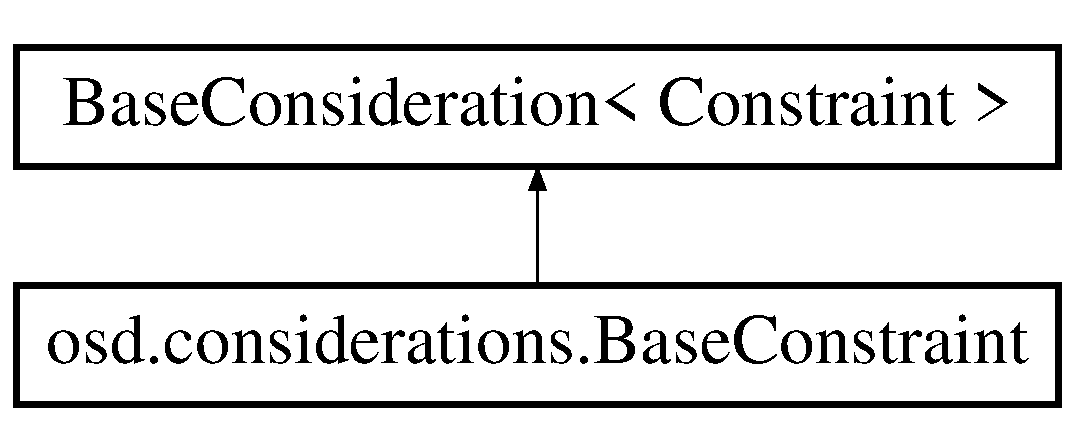
\includegraphics[height=2.000000cm]{interfaceosd_1_1considerations_1_1_base_constraint}
\end{center}
\end{figure}
\subsection*{Public Member Functions}
\begin{DoxyCompactItemize}
\item 
\hypertarget{interfaceosd_1_1considerations_1_1_base_constraint_a5c706c099aecb63a10f270dd1466f169}{default \hyperlink{interfaceosd_1_1considerations_1_1_constraint}{Constraint} {\bfseries bind} (final \hyperlink{interfaceosd_1_1considerations_1_1_lookups}{Lookups} lookups)}\label{interfaceosd_1_1considerations_1_1_base_constraint_a5c706c099aecb63a10f270dd1466f169}

\end{DoxyCompactItemize}


The documentation for this interface was generated from the following file\-:\begin{DoxyCompactItemize}
\item 
/home/travis/build/\-Open-\/\-Source-\/\-Software-\/\-Development/class-\/scheduler/java/src/main/java/osd/considerations/Base\-Constraint.\-java\end{DoxyCompactItemize}

\hypertarget{interfaceosd_1_1considerations_1_1_base_preference}{\section{osd.\-considerations.\-Base\-Preference Interface Reference}
\label{interfaceosd_1_1considerations_1_1_base_preference}\index{osd.\-considerations.\-Base\-Preference@{osd.\-considerations.\-Base\-Preference}}
}
Inheritance diagram for osd.\-considerations.\-Base\-Preference\-:\begin{figure}[H]
\begin{center}
\leavevmode
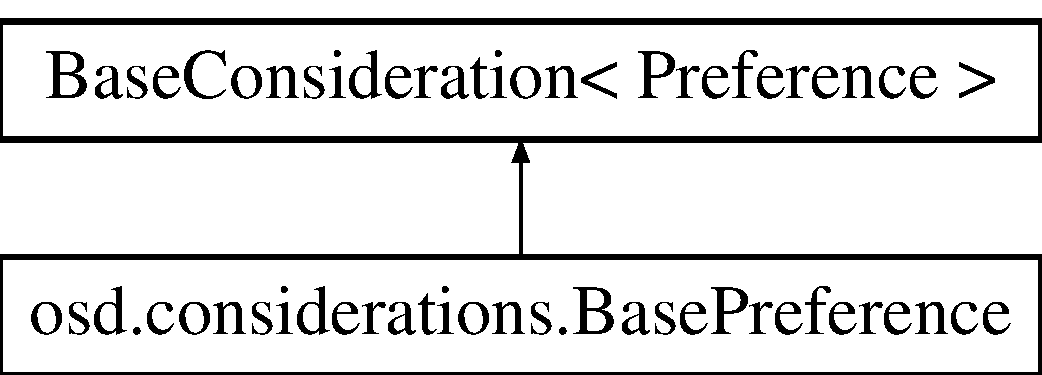
\includegraphics[height=2.000000cm]{interfaceosd_1_1considerations_1_1_base_preference}
\end{center}
\end{figure}
\subsection*{Public Member Functions}
\begin{DoxyCompactItemize}
\item 
int \hyperlink{interfaceosd_1_1considerations_1_1_base_preference_a86c643f9237f9f39eb4b4a0d438f52b6}{worth} ()
\item 
\hypertarget{interfaceosd_1_1considerations_1_1_base_preference_adc9e591207b1d16adf52ad8e7f3b0910}{default \hyperlink{interfaceosd_1_1considerations_1_1_preference}{Preference} {\bfseries bind} (final \hyperlink{interfaceosd_1_1considerations_1_1_lookups}{Lookups} lookups)}\label{interfaceosd_1_1considerations_1_1_base_preference_adc9e591207b1d16adf52ad8e7f3b0910}

\end{DoxyCompactItemize}


\subsection{Member Function Documentation}
\hypertarget{interfaceosd_1_1considerations_1_1_base_preference_a86c643f9237f9f39eb4b4a0d438f52b6}{\index{osd\-::considerations\-::\-Base\-Preference@{osd\-::considerations\-::\-Base\-Preference}!worth@{worth}}
\index{worth@{worth}!osd::considerations::BasePreference@{osd\-::considerations\-::\-Base\-Preference}}
\subsubsection[{worth}]{\setlength{\rightskip}{0pt plus 5cm}int osd.\-considerations.\-Base\-Preference.\-worth (
\begin{DoxyParamCaption}
{}
\end{DoxyParamCaption}
)}}\label{interfaceosd_1_1considerations_1_1_base_preference_a86c643f9237f9f39eb4b4a0d438f52b6}
Determines the \char`\"{}worth\char`\"{} of this base preference. \begin{DoxyReturn}{Returns}
the \char`\"{}worth\char`\"{} of this base preference 
\end{DoxyReturn}
\begin{DoxySeeAlso}{See Also}
Preference\-::worth() 
\end{DoxySeeAlso}


The documentation for this interface was generated from the following file\-:\begin{DoxyCompactItemize}
\item 
/home/travis/build/\-Open-\/\-Source-\/\-Software-\/\-Development/class-\/scheduler/java/src/main/java/osd/considerations/Base\-Preference.\-java\end{DoxyCompactItemize}

\hypertarget{interfaceosd_1_1considerations_1_1_constraint_1_1_blacklist}{\section{osd.\-considerations.\-Constraint.\-Blacklist Interface Reference}
\label{interfaceosd_1_1considerations_1_1_constraint_1_1_blacklist}\index{osd.\-considerations.\-Constraint.\-Blacklist@{osd.\-considerations.\-Constraint.\-Blacklist}}
}
Inheritance diagram for osd.\-considerations.\-Constraint.\-Blacklist\-:\begin{figure}[H]
\begin{center}
\leavevmode
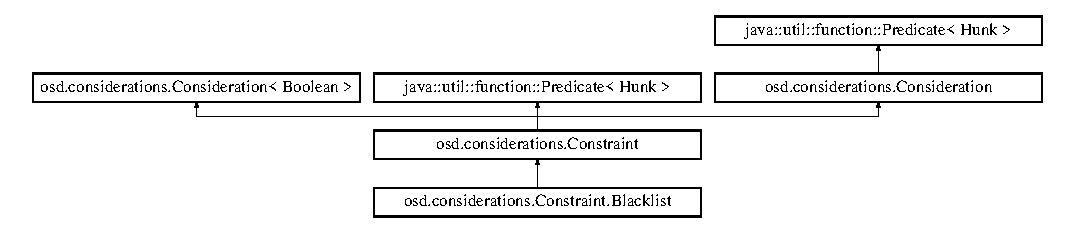
\includegraphics[height=2.685851cm]{interfaceosd_1_1considerations_1_1_constraint_1_1_blacklist}
\end{center}
\end{figure}
\subsection*{Public Member Functions}
\begin{DoxyCompactItemize}
\item 
\hypertarget{interfaceosd_1_1considerations_1_1_constraint_1_1_blacklist_a68f09916ef64b4ee2329f079aa4b26ca}{default Type {\bfseries get\-Type} ()}\label{interfaceosd_1_1considerations_1_1_constraint_1_1_blacklist_a68f09916ef64b4ee2329f079aa4b26ca}

\end{DoxyCompactItemize}
\subsection*{Additional Inherited Members}


The documentation for this interface was generated from the following file\-:\begin{DoxyCompactItemize}
\item 
/home/travis/build/\-Open-\/\-Source-\/\-Software-\/\-Development/class-\/scheduler/src/main/java/osd/considerations/Constraint.\-java\end{DoxyCompactItemize}

\hypertarget{classscheduler_1_1models_1_1_block}{\section{scheduler.\-models.\-Block Class Reference}
\label{classscheduler_1_1models_1_1_block}\index{scheduler.\-models.\-Block@{scheduler.\-models.\-Block}}
}
Inheritance diagram for scheduler.\-models.\-Block\-:\begin{figure}[H]
\begin{center}
\leavevmode
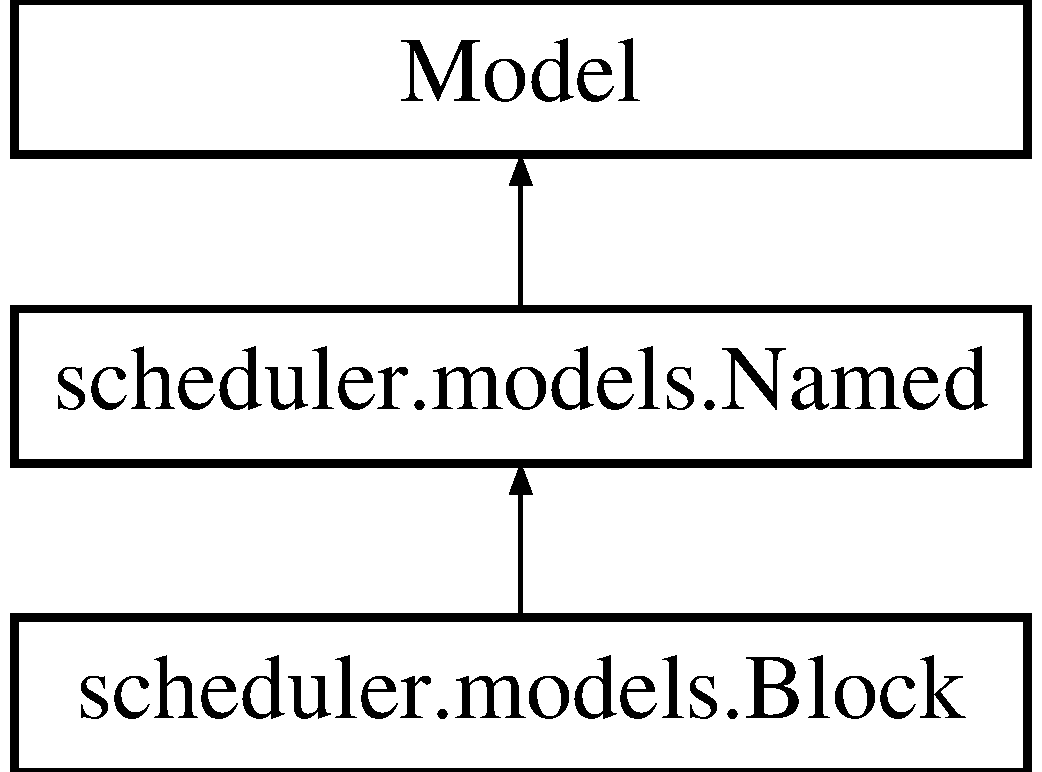
\includegraphics[height=3.000000cm]{classscheduler_1_1models_1_1_block}
\end{center}
\end{figure}
\subsection*{Static Public Attributes}
\begin{DoxyCompactItemize}
\item 
\hypertarget{classscheduler_1_1models_1_1_block_ab78204367b89bd16c9cb000d6bc8ecc6}{tuple {\bfseries next\-\_\-block} = models.\-One\-To\-One\-Field('self', on\-\_\-delete=models.\-C\-A\-S\-C\-A\-D\-E, related\-\_\-name=\char`\"{}previous\-\_\-block\char`\"{}, null=True, blank=True)}\label{classscheduler_1_1models_1_1_block_ab78204367b89bd16c9cb000d6bc8ecc6}

\item 
\hypertarget{classscheduler_1_1models_1_1_block_aa869281bbcdb191ddc5c0ed335e63109}{tuple {\bfseries paired\-\_\-with} = models.\-Foreign\-Key('self', on\-\_\-delete=models.\-C\-A\-S\-C\-A\-D\-E, related\-\_\-name=\char`\"{}paired\-\_\-with\-\_\-reverse\char`\"{}, null=True, blank=True)}\label{classscheduler_1_1models_1_1_block_aa869281bbcdb191ddc5c0ed335e63109}

\end{DoxyCompactItemize}
\subsection*{Additional Inherited Members}


The documentation for this class was generated from the following file\-:\begin{DoxyCompactItemize}
\item 
/home/travis/build/\-Open-\/\-Source-\/\-Software-\/\-Development/class-\/scheduler/mysite/scheduler/models.\-py\end{DoxyCompactItemize}

\hypertarget{interfaceosd_1_1input_1_1_block}{\section{osd.\-input.\-Block Class Reference}
\label{interfaceosd_1_1input_1_1_block}\index{osd.\-input.\-Block@{osd.\-input.\-Block}}
}
Inheritance diagram for osd.\-input.\-Block\-:\begin{figure}[H]
\begin{center}
\leavevmode
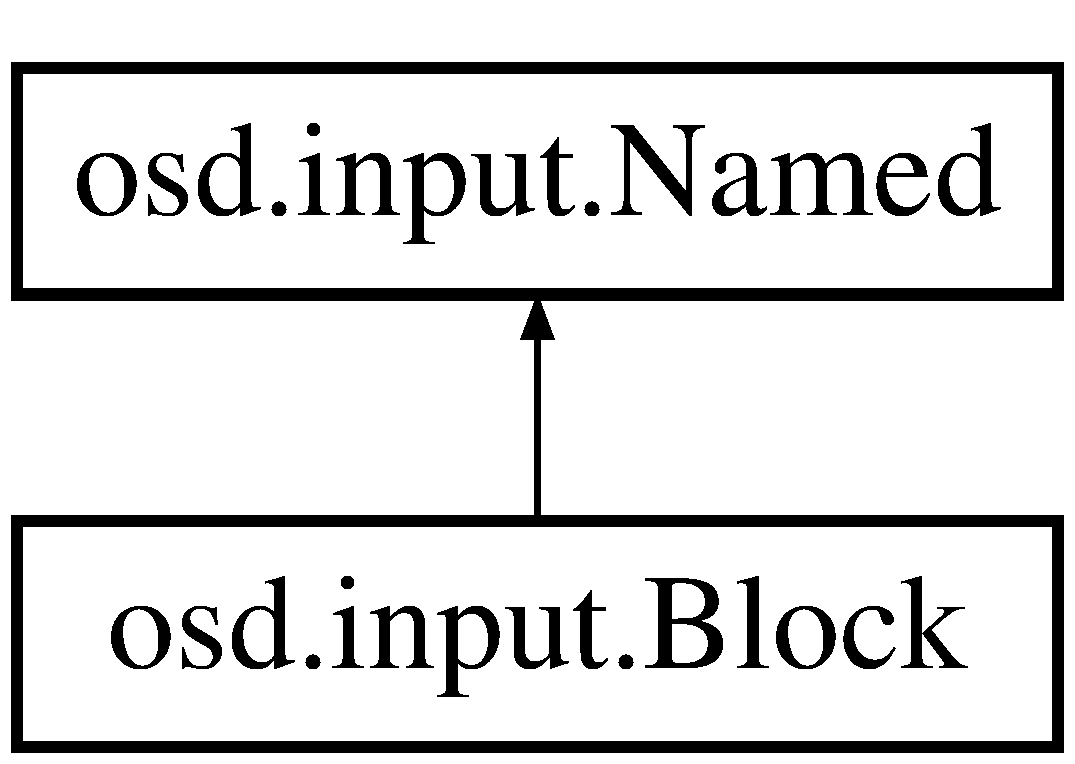
\includegraphics[height=2.000000cm]{interfaceosd_1_1input_1_1_block}
\end{center}
\end{figure}
\subsection*{Public Member Functions}
\begin{DoxyCompactItemize}
\item 
\hyperlink{interfaceosd_1_1input_1_1_block}{Block} \hyperlink{interfaceosd_1_1input_1_1_block_a20c360683729107e2ffe8b2e207448c6}{get\-Next} ()
\item 
\hyperlink{interfaceosd_1_1input_1_1_block}{Block} \hyperlink{interfaceosd_1_1input_1_1_block_a82a4441c85609e3e137db9607bb88126}{get\-Previous} ()
\item 
\hyperlink{interfaceosd_1_1input_1_1_block}{Block} \hyperlink{interfaceosd_1_1input_1_1_block_ab5109873863db50f175e6a41693a1e0e}{get\-Paired\-With} ()
\item 
\hypertarget{interfaceosd_1_1input_1_1_block_a35ce0a9018221268bca81643b0f8f0e8}{{\bfseries Block} (int t\-Block, int t\-Id, int t\-Day, int t\-Time)}\label{interfaceosd_1_1input_1_1_block_a35ce0a9018221268bca81643b0f8f0e8}

\item 
\hypertarget{interfaceosd_1_1input_1_1_block_a974fd00b60c7eccaa2142903d6eb917f}{int {\bfseries get\-Block} ()}\label{interfaceosd_1_1input_1_1_block_a974fd00b60c7eccaa2142903d6eb917f}

\item 
\hypertarget{interfaceosd_1_1input_1_1_block_acd3ebe52ff61c3e0de4f3439474d85aa}{int {\bfseries get\-Id} ()}\label{interfaceosd_1_1input_1_1_block_acd3ebe52ff61c3e0de4f3439474d85aa}

\item 
\hypertarget{interfaceosd_1_1input_1_1_block_a662f746e53305cc8878c36291db446e8}{int {\bfseries get\-Day} ()}\label{interfaceosd_1_1input_1_1_block_a662f746e53305cc8878c36291db446e8}

\item 
\hypertarget{interfaceosd_1_1input_1_1_block_abc2d579a74f45f6b595098555b8ae232}{int {\bfseries get\-Time} ()}\label{interfaceosd_1_1input_1_1_block_abc2d579a74f45f6b595098555b8ae232}

\end{DoxyCompactItemize}


\subsection{Detailed Description}
A specific time block, as specified in the sandbox. A block represents a {\itshape single} contiguous unit of time; if two blocks on different days are assigned the same number, they should be differentiated by an alphabetical suffix (eg. 1\-A and 1\-B). 

\subsection{Member Function Documentation}
\hypertarget{interfaceosd_1_1input_1_1_block_a20c360683729107e2ffe8b2e207448c6}{\index{osd\-::input\-::\-Block@{osd\-::input\-::\-Block}!get\-Next@{get\-Next}}
\index{get\-Next@{get\-Next}!osd::input::Block@{osd\-::input\-::\-Block}}
\subsubsection[{get\-Next}]{\setlength{\rightskip}{0pt plus 5cm}{\bf Block} osd.\-input.\-Block.\-get\-Next (
\begin{DoxyParamCaption}
{}
\end{DoxyParamCaption}
)}}\label{interfaceosd_1_1input_1_1_block_a20c360683729107e2ffe8b2e207448c6}
Gets the next block within the same day. If this is the last block of the day, returns
\begin{DoxyCode}
null 
\end{DoxyCode}
 instead. \begin{DoxyReturn}{Returns}
the next block of the day, or null 
\end{DoxyReturn}
\hypertarget{interfaceosd_1_1input_1_1_block_ab5109873863db50f175e6a41693a1e0e}{\index{osd\-::input\-::\-Block@{osd\-::input\-::\-Block}!get\-Paired\-With@{get\-Paired\-With}}
\index{get\-Paired\-With@{get\-Paired\-With}!osd::input::Block@{osd\-::input\-::\-Block}}
\subsubsection[{get\-Paired\-With}]{\setlength{\rightskip}{0pt plus 5cm}{\bf Block} osd.\-input.\-Block.\-get\-Paired\-With (
\begin{DoxyParamCaption}
{}
\end{DoxyParamCaption}
)}}\label{interfaceosd_1_1input_1_1_block_ab5109873863db50f175e6a41693a1e0e}
Gets the block this one is paired with. For example, block 1\-A would return 1\-B. \begin{DoxyReturn}{Returns}
the block this one is paired with 
\end{DoxyReturn}
\hypertarget{interfaceosd_1_1input_1_1_block_a82a4441c85609e3e137db9607bb88126}{\index{osd\-::input\-::\-Block@{osd\-::input\-::\-Block}!get\-Previous@{get\-Previous}}
\index{get\-Previous@{get\-Previous}!osd::input::Block@{osd\-::input\-::\-Block}}
\subsubsection[{get\-Previous}]{\setlength{\rightskip}{0pt plus 5cm}{\bf Block} osd.\-input.\-Block.\-get\-Previous (
\begin{DoxyParamCaption}
{}
\end{DoxyParamCaption}
)}}\label{interfaceosd_1_1input_1_1_block_a82a4441c85609e3e137db9607bb88126}
Gets the previous block within the same day. If this is the first block of the day, returns
\begin{DoxyCode}
null 
\end{DoxyCode}
 instead. \begin{DoxyReturn}{Returns}
the previous block of the day, or null 
\end{DoxyReturn}


The documentation for this class was generated from the following file\-:\begin{DoxyCompactItemize}
\item 
/home/travis/build/\-Open-\/\-Source-\/\-Software-\/\-Development/class-\/scheduler/java/src/main/java/osd/input/Block.\-java\end{DoxyCompactItemize}

\hypertarget{classosd_1_1database_1_1_block_factory}{\section{osd.\-database.\-Block\-Factory Class Reference}
\label{classosd_1_1database_1_1_block_factory}\index{osd.\-database.\-Block\-Factory@{osd.\-database.\-Block\-Factory}}
}
Inheritance diagram for osd.\-database.\-Block\-Factory\-:\begin{figure}[H]
\begin{center}
\leavevmode
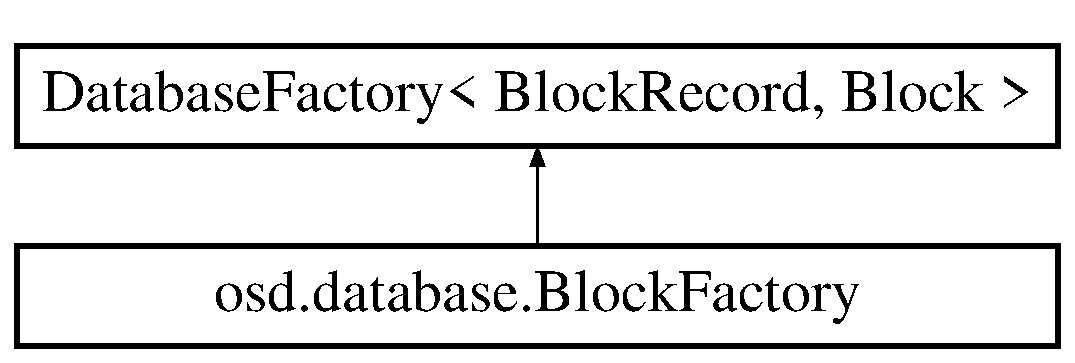
\includegraphics[height=2.000000cm]{classosd_1_1database_1_1_block_factory}
\end{center}
\end{figure}
\subsection*{Public Member Functions}
\begin{DoxyCompactItemize}
\item 
\hypertarget{classosd_1_1database_1_1_block_factory_a47b00ba770d83db998885fa87035f643}{\hyperlink{interfaceosd_1_1input_1_1_block}{Block} {\bfseries create} (final \hyperlink{classosd_1_1database_1_1_block_record}{Block\-Record} record)}\label{classosd_1_1database_1_1_block_factory_a47b00ba770d83db998885fa87035f643}

\end{DoxyCompactItemize}


The documentation for this class was generated from the following file\-:\begin{DoxyCompactItemize}
\item 
/home/travis/build/\-Open-\/\-Source-\/\-Software-\/\-Development/class-\/scheduler/java/src/main/java/osd/database/Block\-Factory.\-java\end{DoxyCompactItemize}

\hypertarget{classscheduler_1_1csv__parser_1_1_block_parser}{\section{scheduler.\-csv\-\_\-parser.\-Block\-Parser Class Reference}
\label{classscheduler_1_1csv__parser_1_1_block_parser}\index{scheduler.\-csv\-\_\-parser.\-Block\-Parser@{scheduler.\-csv\-\_\-parser.\-Block\-Parser}}
}
Inheritance diagram for scheduler.\-csv\-\_\-parser.\-Block\-Parser\-:\begin{figure}[H]
\begin{center}
\leavevmode
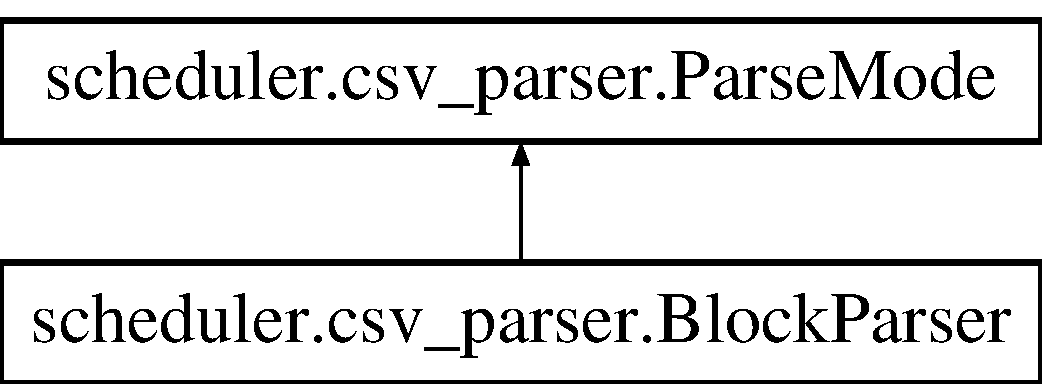
\includegraphics[height=2.000000cm]{classscheduler_1_1csv__parser_1_1_block_parser}
\end{center}
\end{figure}
\subsection*{Public Member Functions}
\begin{DoxyCompactItemize}
\item 
\hypertarget{classscheduler_1_1csv__parser_1_1_block_parser_a9a5711fb09811aa9038259fd3b4fb9f1}{def {\bfseries \-\_\-\-\_\-init\-\_\-\-\_\-}}\label{classscheduler_1_1csv__parser_1_1_block_parser_a9a5711fb09811aa9038259fd3b4fb9f1}

\item 
\hypertarget{classscheduler_1_1csv__parser_1_1_block_parser_a5a628ddc7ec3c88aeab1374c2d292716}{def {\bfseries add\-\_\-row\-\_\-impl}}\label{classscheduler_1_1csv__parser_1_1_block_parser_a5a628ddc7ec3c88aeab1374c2d292716}

\item 
\hypertarget{classscheduler_1_1csv__parser_1_1_block_parser_aef4d6fafd793bdc58454916e8c180ea7}{def {\bfseries get\-\_\-models}}\label{classscheduler_1_1csv__parser_1_1_block_parser_aef4d6fafd793bdc58454916e8c180ea7}

\end{DoxyCompactItemize}
\subsection*{Public Attributes}
\begin{DoxyCompactItemize}
\item 
\hypertarget{classscheduler_1_1csv__parser_1_1_block_parser_ad66ce7569665a2e7fa18757bd667a415}{{\bfseries counts\-\_\-for\-\_\-id}}\label{classscheduler_1_1csv__parser_1_1_block_parser_ad66ce7569665a2e7fa18757bd667a415}

\item 
\hypertarget{classscheduler_1_1csv__parser_1_1_block_parser_a9c7eef3b9448e1bb46784d493f1851a6}{{\bfseries blocks}}\label{classscheduler_1_1csv__parser_1_1_block_parser_a9c7eef3b9448e1bb46784d493f1851a6}

\end{DoxyCompactItemize}
\subsection*{Static Public Attributes}
\begin{DoxyCompactItemize}
\item 
\hypertarget{classscheduler_1_1csv__parser_1_1_block_parser_ac276431a1f6649ead463ce5bbfc998eb}{tuple {\bfseries columns} = (\char`\"{}id\char`\"{}, \char`\"{}day\char`\"{}, \char`\"{}start\char`\"{}, \char`\"{}end\char`\"{})}\label{classscheduler_1_1csv__parser_1_1_block_parser_ac276431a1f6649ead463ce5bbfc998eb}

\item 
\hypertarget{classscheduler_1_1csv__parser_1_1_block_parser_a1079ac8a21cbc2d30fa675f0e4d79097}{tuple {\bfseries suffixes} = (\char`\"{}A\char`\"{}, \char`\"{}B\char`\"{})}\label{classscheduler_1_1csv__parser_1_1_block_parser_a1079ac8a21cbc2d30fa675f0e4d79097}

\end{DoxyCompactItemize}


The documentation for this class was generated from the following file\-:\begin{DoxyCompactItemize}
\item 
/home/travis/build/\-Open-\/\-Source-\/\-Software-\/\-Development/class-\/scheduler/mysite/scheduler/csv\-\_\-parser.\-py\end{DoxyCompactItemize}

\hypertarget{classosd_1_1database_1_1_block_record}{\section{osd.\-database.\-Block\-Record Class Reference}
\label{classosd_1_1database_1_1_block_record}\index{osd.\-database.\-Block\-Record@{osd.\-database.\-Block\-Record}}
}


The documentation for this class was generated from the following file\-:\begin{DoxyCompactItemize}
\item 
/home/travis/build/\-Open-\/\-Source-\/\-Software-\/\-Development/class-\/scheduler/java/src/main/java/osd/database/Block\-Record.\-java\end{DoxyCompactItemize}

\hypertarget{classosd_1_1input_1_1_block_set}{\section{osd.\-input.\-Block\-Set Class Reference}
\label{classosd_1_1input_1_1_block_set}\index{osd.\-input.\-Block\-Set@{osd.\-input.\-Block\-Set}}
}
\subsection*{Public Member Functions}
\begin{DoxyCompactItemize}
\item 
\hypertarget{classosd_1_1input_1_1_block_set_a8fd250a4e0e3a3e750c9b196126b8d3f}{{\bfseries Block\-Set} (\hyperlink{interfaceosd_1_1input_1_1_block}{Block} a, \hyperlink{interfaceosd_1_1input_1_1_block}{Block} b, int t\-Id)}\label{classosd_1_1input_1_1_block_set_a8fd250a4e0e3a3e750c9b196126b8d3f}

\item 
\hypertarget{classosd_1_1input_1_1_block_set_a3783ae61ef0ac617b7a1a0bd8a7429b2}{Boolean {\bfseries get\-Is\-Whole} ()}\label{classosd_1_1input_1_1_block_set_a3783ae61ef0ac617b7a1a0bd8a7429b2}

\item 
\hypertarget{classosd_1_1input_1_1_block_set_a181c7721e45b3436f2fbf250016b84ca}{void {\bfseries set\-Is\-Whole} (Boolean is\-Whole)}\label{classosd_1_1input_1_1_block_set_a181c7721e45b3436f2fbf250016b84ca}

\item 
\hypertarget{classosd_1_1input_1_1_block_set_afee566d5e4864c98efbcd1905d8b6e2d}{\hyperlink{interfaceosd_1_1input_1_1_block}{Block} {\bfseries get\-Block\-A} ()}\label{classosd_1_1input_1_1_block_set_afee566d5e4864c98efbcd1905d8b6e2d}

\item 
\hypertarget{classosd_1_1input_1_1_block_set_a2afd5bc8227b04f9894fd4dc417fbfc9}{\hyperlink{interfaceosd_1_1input_1_1_block}{Block} {\bfseries get\-Block\-B} ()}\label{classosd_1_1input_1_1_block_set_a2afd5bc8227b04f9894fd4dc417fbfc9}

\item 
\hypertarget{classosd_1_1input_1_1_block_set_a38c5a636d48e3282af25c15f2269f2f5}{int {\bfseries get\-Id} ()}\label{classosd_1_1input_1_1_block_set_a38c5a636d48e3282af25c15f2269f2f5}

\end{DoxyCompactItemize}


The documentation for this class was generated from the following file\-:\begin{DoxyCompactItemize}
\item 
/home/travis/build/\-Open-\/\-Source-\/\-Software-\/\-Development/class-\/scheduler/src/main/java/osd/input/Block\-Set.\-java\end{DoxyCompactItemize}

\hypertarget{interfaceosd_1_1output_1_1_callbacks}{\section{osd.\-output.\-Callbacks Interface Reference}
\label{interfaceosd_1_1output_1_1_callbacks}\index{osd.\-output.\-Callbacks@{osd.\-output.\-Callbacks}}
}


Inherited by osd.\-main.\-Demo\-Callbacks.

\subsection*{Public Member Functions}
\begin{DoxyCompactItemize}
\item 
boolean \hyperlink{interfaceosd_1_1output_1_1_callbacks_a9ddd7287b111fb9ae7b2f8c6f37f5b7c}{stop\-Condition} ()
\item 
void \hyperlink{interfaceosd_1_1output_1_1_callbacks_aee68de08f891ebec0aca383dd2b8a1b5}{on\-Complete\-Result} (final \hyperlink{interfaceosd_1_1output_1_1_results}{Results} results)
\item 
\hypertarget{interfaceosd_1_1output_1_1_callbacks_a60180d47bf100b056467ce6397702b2b}{void {\bfseries on\-Backtrack} (final \hyperlink{interfaceosd_1_1output_1_1_results}{Results} results)}\label{interfaceosd_1_1output_1_1_callbacks_a60180d47bf100b056467ce6397702b2b}

\end{DoxyCompactItemize}


\subsection{Member Function Documentation}
\hypertarget{interfaceosd_1_1output_1_1_callbacks_aee68de08f891ebec0aca383dd2b8a1b5}{\index{osd\-::output\-::\-Callbacks@{osd\-::output\-::\-Callbacks}!on\-Complete\-Result@{on\-Complete\-Result}}
\index{on\-Complete\-Result@{on\-Complete\-Result}!osd::output::Callbacks@{osd\-::output\-::\-Callbacks}}
\subsubsection[{on\-Complete\-Result}]{\setlength{\rightskip}{0pt plus 5cm}void osd.\-output.\-Callbacks.\-on\-Complete\-Result (
\begin{DoxyParamCaption}
\item[{final {\bf Results}}]{results}
\end{DoxyParamCaption}
)}}\label{interfaceosd_1_1output_1_1_callbacks_aee68de08f891ebec0aca383dd2b8a1b5}
Called whenever the algorithm generates a complete result. 
\begin{DoxyParams}{Parameters}
{\em results} & the complete \hyperlink{interfaceosd_1_1output_1_1_results}{result} \\
\hline
\end{DoxyParams}
\hypertarget{interfaceosd_1_1output_1_1_callbacks_a9ddd7287b111fb9ae7b2f8c6f37f5b7c}{\index{osd\-::output\-::\-Callbacks@{osd\-::output\-::\-Callbacks}!stop\-Condition@{stop\-Condition}}
\index{stop\-Condition@{stop\-Condition}!osd::output::Callbacks@{osd\-::output\-::\-Callbacks}}
\subsubsection[{stop\-Condition}]{\setlength{\rightskip}{0pt plus 5cm}boolean osd.\-output.\-Callbacks.\-stop\-Condition (
\begin{DoxyParamCaption}
{}
\end{DoxyParamCaption}
)}}\label{interfaceosd_1_1output_1_1_callbacks_a9ddd7287b111fb9ae7b2f8c6f37f5b7c}
Indicate whether we're satisfied with the results we've received. \begin{DoxyReturn}{Returns}
whether we're satisfied with the results we've received 
\end{DoxyReturn}


The documentation for this interface was generated from the following file\-:\begin{DoxyCompactItemize}
\item 
/home/travis/build/\-Open-\/\-Source-\/\-Software-\/\-Development/class-\/scheduler/java/src/main/java/osd/output/Callbacks.\-java\end{DoxyCompactItemize}

\hypertarget{classimport__faculty__data_1_1_command}{\section{import\-\_\-faculty\-\_\-data.\-Command Class Reference}
\label{classimport__faculty__data_1_1_command}\index{import\-\_\-faculty\-\_\-data.\-Command@{import\-\_\-faculty\-\_\-data.\-Command}}
}
Inheritance diagram for import\-\_\-faculty\-\_\-data.\-Command\-:\begin{figure}[H]
\begin{center}
\leavevmode
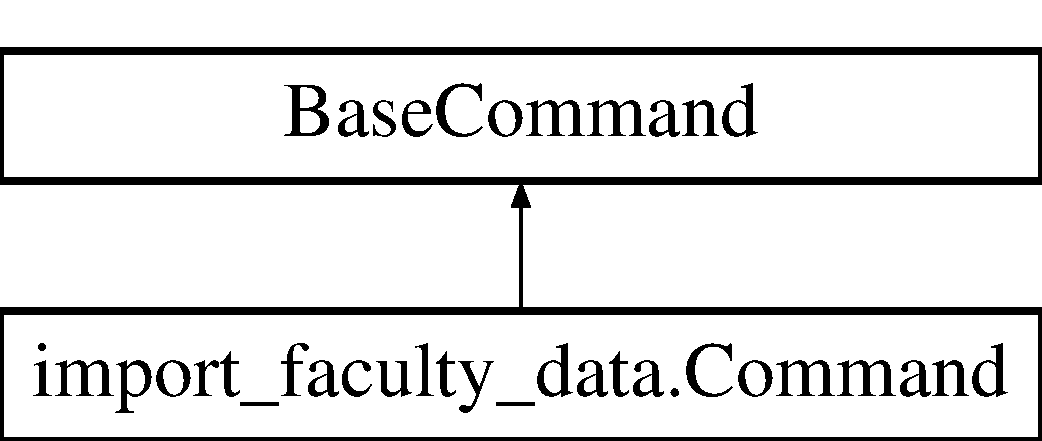
\includegraphics[height=2.000000cm]{classimport__faculty__data_1_1_command}
\end{center}
\end{figure}
\subsection*{Public Member Functions}
\begin{DoxyCompactItemize}
\item 
\hypertarget{classimport__faculty__data_1_1_command_ac257d9fe1b3408228ef8d5c291be6151}{def {\bfseries import\-\_\-faculty\-\_\-from\-\_\-csv\-\_\-file}}\label{classimport__faculty__data_1_1_command_ac257d9fe1b3408228ef8d5c291be6151}

\item 
def \hyperlink{classimport__faculty__data_1_1_command_a7ef6e803136bb954d64f6a54401b31b9}{handle}
\end{DoxyCompactItemize}


\subsection{Member Function Documentation}
\hypertarget{classimport__faculty__data_1_1_command_a7ef6e803136bb954d64f6a54401b31b9}{\index{import\-\_\-faculty\-\_\-data\-::\-Command@{import\-\_\-faculty\-\_\-data\-::\-Command}!handle@{handle}}
\index{handle@{handle}!import_faculty_data::Command@{import\-\_\-faculty\-\_\-data\-::\-Command}}
\subsubsection[{handle}]{\setlength{\rightskip}{0pt plus 5cm}def import\-\_\-faculty\-\_\-data.\-Command.\-handle (
\begin{DoxyParamCaption}
\item[{}]{self, }
\item[{}]{args, }
\item[{}]{options}
\end{DoxyParamCaption}
)}}\label{classimport__faculty__data_1_1_command_a7ef6e803136bb954d64f6a54401b31b9}
\begin{DoxyVerb}Call the function to import data
\end{DoxyVerb}
 

The documentation for this class was generated from the following file\-:\begin{DoxyCompactItemize}
\item 
/home/travis/build/\-Open-\/\-Source-\/\-Software-\/\-Development/class-\/scheduler/mysite/faculty\-\_\-data/management/commands/import\-\_\-faculty\-\_\-data.\-py\end{DoxyCompactItemize}

\hypertarget{classimport__room__data_1_1_command}{\section{import\-\_\-room\-\_\-data.\-Command Class Reference}
\label{classimport__room__data_1_1_command}\index{import\-\_\-room\-\_\-data.\-Command@{import\-\_\-room\-\_\-data.\-Command}}
}
Inheritance diagram for import\-\_\-room\-\_\-data.\-Command\-:\begin{figure}[H]
\begin{center}
\leavevmode
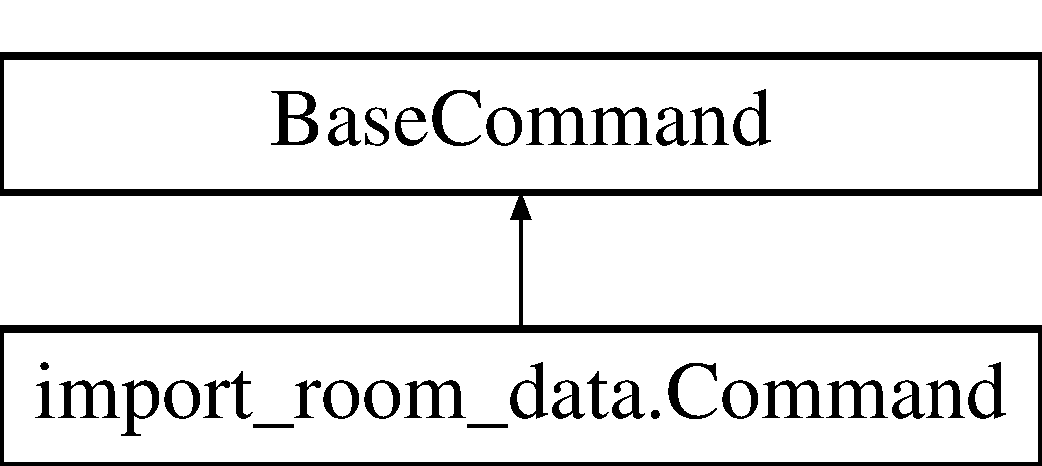
\includegraphics[height=2.000000cm]{classimport__room__data_1_1_command}
\end{center}
\end{figure}
\subsection*{Public Member Functions}
\begin{DoxyCompactItemize}
\item 
\hypertarget{classimport__room__data_1_1_command_a6072ecb4a6cba32f7c36a8307bec0cdb}{def {\bfseries import\-\_\-room\-\_\-from\-\_\-csv\-\_\-file}}\label{classimport__room__data_1_1_command_a6072ecb4a6cba32f7c36a8307bec0cdb}

\item 
def \hyperlink{classimport__room__data_1_1_command_a6b1b74cc5acad3b1e666909c6d46f96c}{handle}
\end{DoxyCompactItemize}


\subsection{Member Function Documentation}
\hypertarget{classimport__room__data_1_1_command_a6b1b74cc5acad3b1e666909c6d46f96c}{\index{import\-\_\-room\-\_\-data\-::\-Command@{import\-\_\-room\-\_\-data\-::\-Command}!handle@{handle}}
\index{handle@{handle}!import_room_data::Command@{import\-\_\-room\-\_\-data\-::\-Command}}
\subsubsection[{handle}]{\setlength{\rightskip}{0pt plus 5cm}def import\-\_\-room\-\_\-data.\-Command.\-handle (
\begin{DoxyParamCaption}
\item[{}]{self, }
\item[{}]{args, }
\item[{}]{options}
\end{DoxyParamCaption}
)}}\label{classimport__room__data_1_1_command_a6b1b74cc5acad3b1e666909c6d46f96c}
\begin{DoxyVerb}Call the function to import data
\end{DoxyVerb}
 

The documentation for this class was generated from the following file\-:\begin{DoxyCompactItemize}
\item 
/home/travis/build/\-Open-\/\-Source-\/\-Software-\/\-Development/class-\/scheduler/mysite/room\-\_\-data/management/commands/import\-\_\-room\-\_\-data.\-py\end{DoxyCompactItemize}

\hypertarget{interfaceosd_1_1considerations_1_1_consideration}{\section{osd.\-considerations.\-Consideration Interface Reference}
\label{interfaceosd_1_1considerations_1_1_consideration}\index{osd.\-considerations.\-Consideration@{osd.\-considerations.\-Consideration}}
}
Inheritance diagram for osd.\-considerations.\-Consideration\-:\begin{figure}[H]
\begin{center}
\leavevmode
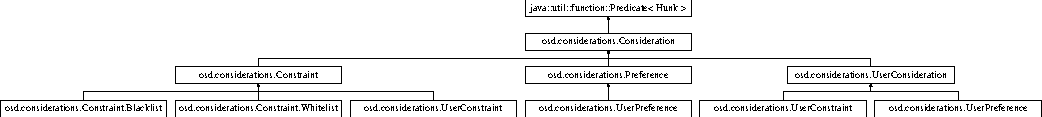
\includegraphics[height=1.575246cm]{interfaceosd_1_1considerations_1_1_consideration}
\end{center}
\end{figure}


\subsection{Detailed Description}
Superinterface for preferences and constraints. When you see \char`\"{}consideration\char`\"{} in the docs, read it as \char`\"{}preference\char`\"{} or \char`\"{}constraint\char`\"{} as appropriate. 

The documentation for this interface was generated from the following file\-:\begin{DoxyCompactItemize}
\item 
/home/travis/build/\-Open-\/\-Source-\/\-Software-\/\-Development/class-\/scheduler/java/src/main/java/osd/considerations/Consideration.\-java\end{DoxyCompactItemize}

\hypertarget{interfaceosd_1_1considerations_1_1_consideration_3_01_t_01_4}{\section{osd.\-considerations.\-Consideration$<$ T $>$ Interface Reference}
\label{interfaceosd_1_1considerations_1_1_consideration_3_01_t_01_4}\index{osd.\-considerations.\-Consideration$<$ T $>$@{osd.\-considerations.\-Consideration$<$ T $>$}}
}
Inheritance diagram for osd.\-considerations.\-Consideration$<$ T $>$\-:\begin{figure}[H]
\begin{center}
\leavevmode
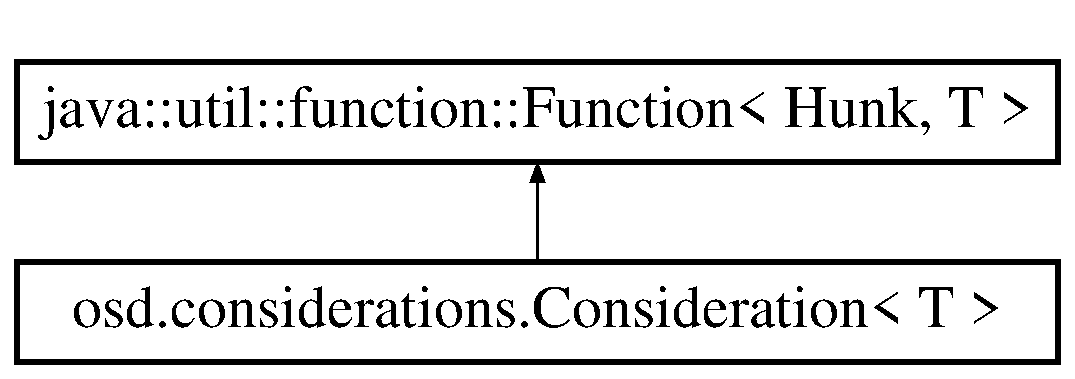
\includegraphics[height=2.000000cm]{interfaceosd_1_1considerations_1_1_consideration_3_01_t_01_4}
\end{center}
\end{figure}
\subsection*{Public Member Functions}
\begin{DoxyCompactItemize}
\item 
\hypertarget{interfaceosd_1_1considerations_1_1_consideration_3_01_t_01_4_a89b752c3950fb30f7a98d412bb413094}{T {\bfseries evaluate} (final \hyperlink{classosd_1_1output_1_1_hunk}{Hunk} hunk)}\label{interfaceosd_1_1considerations_1_1_consideration_3_01_t_01_4_a89b752c3950fb30f7a98d412bb413094}

\item 
\hypertarget{interfaceosd_1_1considerations_1_1_consideration_3_01_t_01_4_a2f414e91c45335e5284c5aa7fd064c41}{default T {\bfseries apply} (final \hyperlink{classosd_1_1output_1_1_hunk}{Hunk} hunk)}\label{interfaceosd_1_1considerations_1_1_consideration_3_01_t_01_4_a2f414e91c45335e5284c5aa7fd064c41}

\end{DoxyCompactItemize}


\subsection{Detailed Description}
Superinterface for user preferences and user constraints. 

The documentation for this interface was generated from the following file\-:\begin{DoxyCompactItemize}
\item 
/home/travis/build/\-Open-\/\-Source-\/\-Software-\/\-Development/class-\/scheduler/src/main/java/osd/considerations/Consideration.\-java\end{DoxyCompactItemize}

\hypertarget{interfaceosd_1_1considerations_1_1_constraint}{\section{osd.\-considerations.\-Constraint Interface Reference}
\label{interfaceosd_1_1considerations_1_1_constraint}\index{osd.\-considerations.\-Constraint@{osd.\-considerations.\-Constraint}}
}
Inheritance diagram for osd.\-considerations.\-Constraint\-:\begin{figure}[H]
\begin{center}
\leavevmode
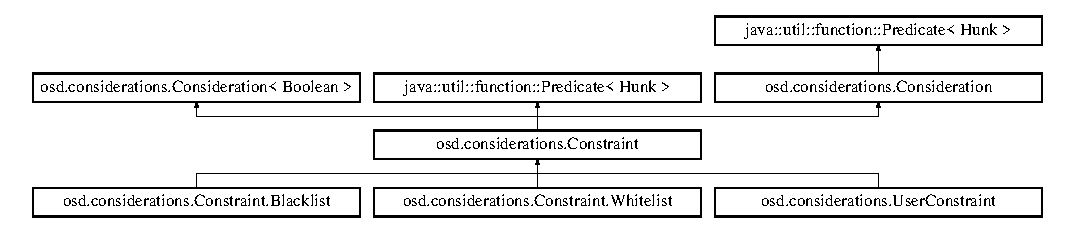
\includegraphics[height=2.685851cm]{interfaceosd_1_1considerations_1_1_constraint}
\end{center}
\end{figure}
\subsection*{Classes}
\begin{DoxyCompactItemize}
\item 
interface \hyperlink{interfaceosd_1_1considerations_1_1_constraint_1_1_blacklist}{Blacklist}
\item 
enum {\bfseries Type}
\item 
interface \hyperlink{interfaceosd_1_1considerations_1_1_constraint_1_1_whitelist}{Whitelist}
\end{DoxyCompactItemize}
\subsection*{Public Member Functions}
\begin{DoxyCompactItemize}
\item 
boolean \hyperlink{interfaceosd_1_1considerations_1_1_constraint_a50c53a0c89a4cfb8b58deae081ca3787}{test} (final \hyperlink{classosd_1_1output_1_1_hunk}{Hunk} hunk)
\item 
\hypertarget{interfaceosd_1_1considerations_1_1_constraint_ac20b9d39e2b0e9fca84c71603af9ad46}{Type {\bfseries get\-Type} ()}\label{interfaceosd_1_1considerations_1_1_constraint_ac20b9d39e2b0e9fca84c71603af9ad46}

\item 
\hypertarget{interfaceosd_1_1considerations_1_1_constraint_a36bc96efdaadd6f5bcf64198ccf97cd6}{default boolean {\bfseries test} (final \hyperlink{classosd_1_1output_1_1_hunk}{Hunk} hunk)}\label{interfaceosd_1_1considerations_1_1_constraint_a36bc96efdaadd6f5bcf64198ccf97cd6}

\end{DoxyCompactItemize}
\subsection*{Static Public Member Functions}
\begin{DoxyCompactItemize}
\item 
\hypertarget{interfaceosd_1_1considerations_1_1_constraint_aa9c71385c629e7bc5d9361f707d39622}{static \hyperlink{interfaceosd_1_1considerations_1_1_constraint}{Constraint} {\bfseries of} (final Predicate$<$ Boolean $>$ predicate, final Type type)}\label{interfaceosd_1_1considerations_1_1_constraint_aa9c71385c629e7bc5d9361f707d39622}

\end{DoxyCompactItemize}


\subsection{Detailed Description}
A predicate over hunks. 

Since hunks are used as both output and internally during scheduling, it is possible that some members of a hunk may be
\begin{DoxyCode}
null 
\end{DoxyCode}
 . If a constraint attempts to refer to some member of a hunk for which that member is
\begin{DoxyCode}
null 
\end{DoxyCode}
 , the constraint msut return
\begin{DoxyCode}
\textcolor{keyword}{true} 
\end{DoxyCode}
 .

\subsection{Member Function Documentation}
\hypertarget{interfaceosd_1_1considerations_1_1_constraint_a50c53a0c89a4cfb8b58deae081ca3787}{\index{osd\-::considerations\-::\-Constraint@{osd\-::considerations\-::\-Constraint}!test@{test}}
\index{test@{test}!osd::considerations::Constraint@{osd\-::considerations\-::\-Constraint}}
\subsubsection[{test}]{\setlength{\rightskip}{0pt plus 5cm}boolean osd.\-considerations.\-Constraint.\-test (
\begin{DoxyParamCaption}
\item[{final {\bf Hunk}}]{hunk}
\end{DoxyParamCaption}
)}}\label{interfaceosd_1_1considerations_1_1_constraint_a50c53a0c89a4cfb8b58deae081ca3787}
Determines whether some hunk satisfies this consideration. If the consideration is indeterminate because the hunk contains
\begin{DoxyCode}
null 
\end{DoxyCode}
 s, the result must be
\begin{DoxyCode}
\textcolor{keyword}{true} 
\end{DoxyCode}
 . 
\begin{DoxyParams}{Parameters}
{\em hunk} & a hunk \\
\hline
\end{DoxyParams}
\begin{DoxyReturn}{Returns}
true if the hunk passes or is indeterminate, false if it fails 
\end{DoxyReturn}


Implemented in \hyperlink{classosd_1_1considerations_1_1_user_constraint_a9378d413848106a42ede0782730c0408}{osd.\-considerations.\-User\-Constraint}.



The documentation for this interface was generated from the following file\-:\begin{DoxyCompactItemize}
\item 
/home/travis/build/\-Open-\/\-Source-\/\-Software-\/\-Development/class-\/scheduler/java/src/main/java/osd/considerations/Constraint.\-java\end{DoxyCompactItemize}

\hypertarget{interfaceosd_1_1input_1_1_course}{\section{osd.\-input.\-Course Class Reference}
\label{interfaceosd_1_1input_1_1_course}\index{osd.\-input.\-Course@{osd.\-input.\-Course}}
}
Inheritance diagram for osd.\-input.\-Course\-:\begin{figure}[H]
\begin{center}
\leavevmode
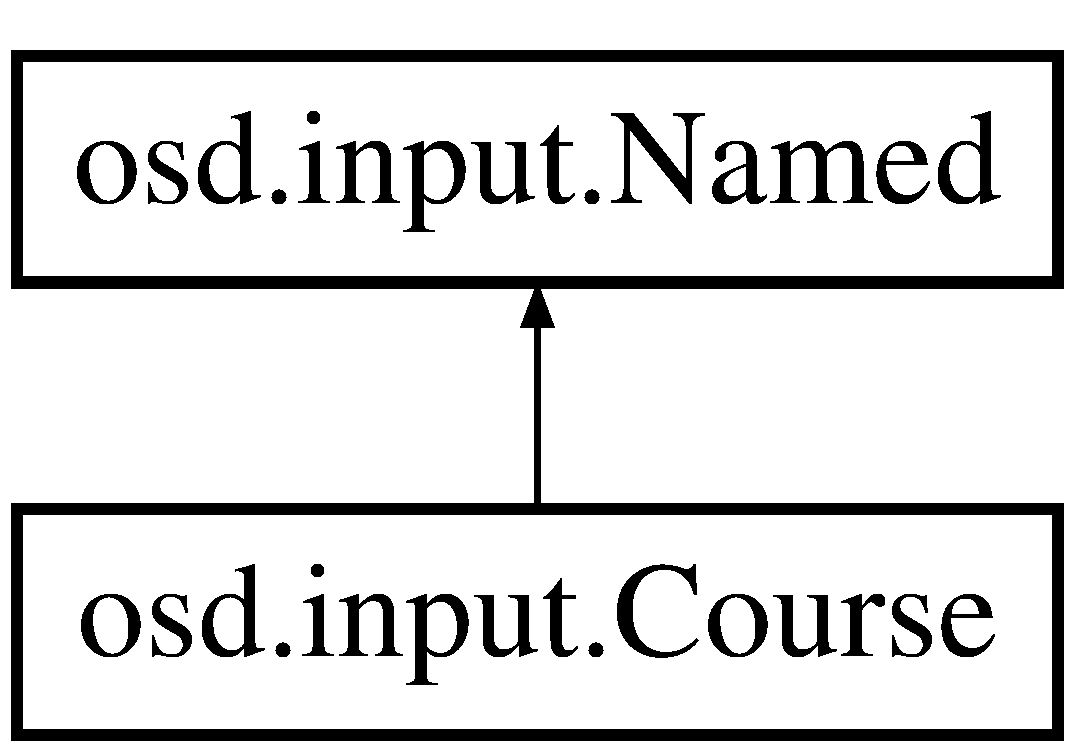
\includegraphics[height=2.000000cm]{interfaceosd_1_1input_1_1_course}
\end{center}
\end{figure}
\subsection*{Public Member Functions}
\begin{DoxyCompactItemize}
\item 
Iterable$<$ \hyperlink{interfaceosd_1_1input_1_1_section}{Section} $>$ \hyperlink{interfaceosd_1_1input_1_1_course_ad8e1f791bfa78ae2cca7fda58135abb3}{get\-Sections} ()
\item 
\hypertarget{interfaceosd_1_1input_1_1_course_a200dcd97e20382d4ac5ca3732e2f84e0}{{\bfseries Course} (int t\-Student\-Int, String t\-Course\-Id, String t\-Div\-Id, \hyperlink{interfaceosd_1_1input_1_1_room_type}{Room\-Type} t\-Room\-Req, int t\-Level, int t\-Sec\-Capacity)}\label{interfaceosd_1_1input_1_1_course_a200dcd97e20382d4ac5ca3732e2f84e0}

\item 
\hypertarget{interfaceosd_1_1input_1_1_course_ac1dcc39824df2cddceb725fe8531bec3}{int {\bfseries get\-Student\-Int} ()}\label{interfaceosd_1_1input_1_1_course_ac1dcc39824df2cddceb725fe8531bec3}

\item 
\hypertarget{interfaceosd_1_1input_1_1_course_a44efc9e443011bb27cb6a87d472ee975}{String {\bfseries get\-Course\-Id} ()}\label{interfaceosd_1_1input_1_1_course_a44efc9e443011bb27cb6a87d472ee975}

\item 
\hypertarget{interfaceosd_1_1input_1_1_course_a741123d10fa05510e8ffe793c2bbb2c3}{String {\bfseries get\-Div\-Id} ()}\label{interfaceosd_1_1input_1_1_course_a741123d10fa05510e8ffe793c2bbb2c3}

\item 
\hypertarget{interfaceosd_1_1input_1_1_course_a79f3e81e08205484f6858c56f988c2f2}{\hyperlink{interfaceosd_1_1input_1_1_room_type}{Room\-Type} {\bfseries get\-Room\-Req} ()}\label{interfaceosd_1_1input_1_1_course_a79f3e81e08205484f6858c56f988c2f2}

\item 
\hypertarget{interfaceosd_1_1input_1_1_course_ab24a202369530a57e1c0693d3eb26b2d}{int {\bfseries get\-Level} ()}\label{interfaceosd_1_1input_1_1_course_ab24a202369530a57e1c0693d3eb26b2d}

\item 
\hypertarget{interfaceosd_1_1input_1_1_course_a8d56da278fcb942ffd7427a9865fb3ea}{int {\bfseries get\-Section\-Capacity} ()}\label{interfaceosd_1_1input_1_1_course_a8d56da278fcb942ffd7427a9865fb3ea}

\end{DoxyCompactItemize}


\subsection{Detailed Description}
Represents a specific course. The most important element of a course is its sections, so that's what this focuses on. 

\subsection{Member Function Documentation}
\hypertarget{interfaceosd_1_1input_1_1_course_ad8e1f791bfa78ae2cca7fda58135abb3}{\index{osd\-::input\-::\-Course@{osd\-::input\-::\-Course}!get\-Sections@{get\-Sections}}
\index{get\-Sections@{get\-Sections}!osd::input::Course@{osd\-::input\-::\-Course}}
\subsubsection[{get\-Sections}]{\setlength{\rightskip}{0pt plus 5cm}Iterable$<${\bf Section}$>$ osd.\-input.\-Course.\-get\-Sections (
\begin{DoxyParamCaption}
{}
\end{DoxyParamCaption}
)}}\label{interfaceosd_1_1input_1_1_course_ad8e1f791bfa78ae2cca7fda58135abb3}
Returns all the sections for this course. This should consider both \char`\"{}pregenerated\char`\"{} sections specified in the database, and \char`\"{}additional\char`\"{} sections specified in the course's \char`\"{}sections\char`\"{} column. \begin{DoxyReturn}{Returns}
an iterable representing this course's sections 
\end{DoxyReturn}


The documentation for this class was generated from the following file\-:\begin{DoxyCompactItemize}
\item 
/home/travis/build/\-Open-\/\-Source-\/\-Software-\/\-Development/class-\/scheduler/java/src/main/java/osd/input/Course.\-java\end{DoxyCompactItemize}

\hypertarget{classscheduler_1_1models_1_1_course}{\section{scheduler.\-models.\-Course Class Reference}
\label{classscheduler_1_1models_1_1_course}\index{scheduler.\-models.\-Course@{scheduler.\-models.\-Course}}
}
Inheritance diagram for scheduler.\-models.\-Course\-:\begin{figure}[H]
\begin{center}
\leavevmode
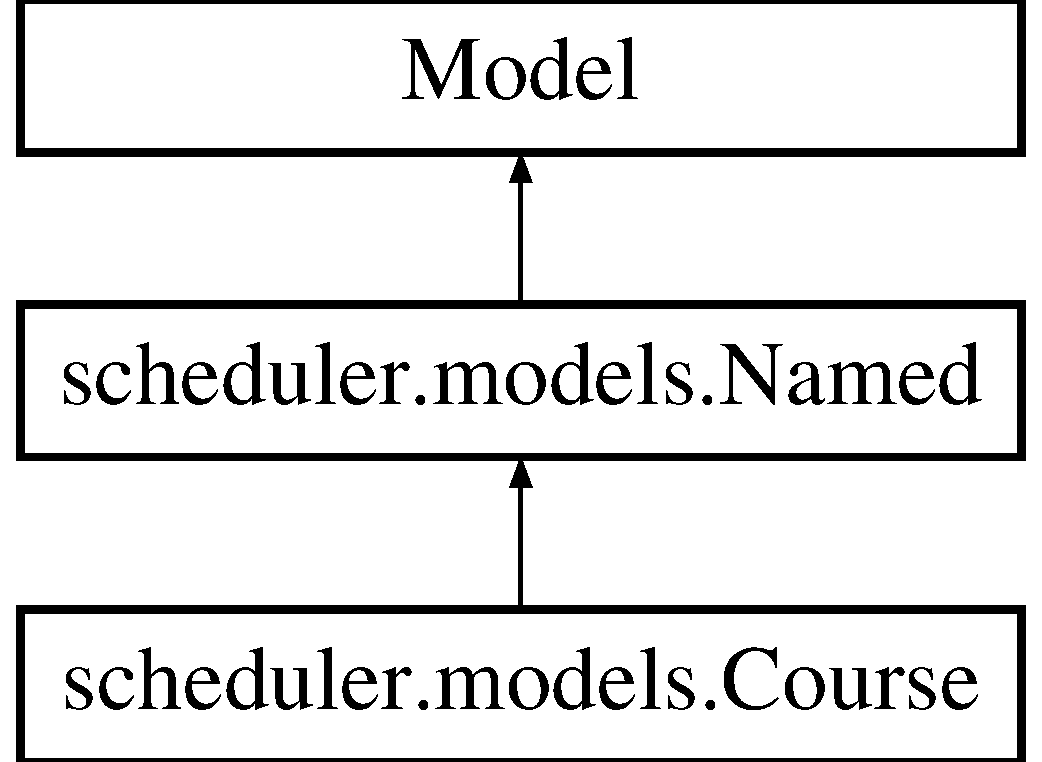
\includegraphics[height=3.000000cm]{classscheduler_1_1models_1_1_course}
\end{center}
\end{figure}
\subsection*{Static Public Attributes}
\begin{DoxyCompactItemize}
\item 
\hypertarget{classscheduler_1_1models_1_1_course_a469fbc25ba99da1185556bcd2d46f1b0}{tuple {\bfseries division} = models.\-Foreign\-Key(\hyperlink{classscheduler_1_1models_1_1_division}{Division}, on\-\_\-delete=models.\-C\-A\-S\-C\-A\-D\-E)}\label{classscheduler_1_1models_1_1_course_a469fbc25ba99da1185556bcd2d46f1b0}

\item 
\hypertarget{classscheduler_1_1models_1_1_course_a6a226c9c7cf238182071b5e00796af9a}{tuple {\bfseries program} = models.\-Char\-Field(max\-\_\-length=10)}\label{classscheduler_1_1models_1_1_course_a6a226c9c7cf238182071b5e00796af9a}

\item 
\hypertarget{classscheduler_1_1models_1_1_course_a1adc8da7f3f21d51f6262caea84123d7}{tuple {\bfseries title} = models.\-Char\-Field(max\-\_\-length=30, null=True, blank=True)}\label{classscheduler_1_1models_1_1_course_a1adc8da7f3f21d51f6262caea84123d7}

\item 
\hypertarget{classscheduler_1_1models_1_1_course_adcee98a824c0827372f76dd17d342409}{tuple {\bfseries ins\-\_\-method} = models.\-Char\-Field(max\-\_\-length=20, null=True, blank=True)}\label{classscheduler_1_1models_1_1_course_adcee98a824c0827372f76dd17d342409}

\item 
\hypertarget{classscheduler_1_1models_1_1_course_a8ea6f27aab56095042c8ef51b7715341}{tuple {\bfseries section\-\_\-capacity} = models.\-Positive\-Integer\-Field()}\label{classscheduler_1_1models_1_1_course_a8ea6f27aab56095042c8ef51b7715341}

\item 
\hypertarget{classscheduler_1_1models_1_1_course_a2d8ee964882dee311d4734297cb6c91b}{tuple {\bfseries style} = models.\-Char\-Field(max\-\_\-length=20, null=True, blank=True)}\label{classscheduler_1_1models_1_1_course_a2d8ee964882dee311d4734297cb6c91b}

\end{DoxyCompactItemize}
\subsection*{Additional Inherited Members}


\subsection{Detailed Description}
\begin{DoxyVerb}    Table: Course
    Primary Key: Composite (program, identifier)
    Columns:
        division: Foreign Key (Division)
            - The course's division code (ex: ITS)
        program: CharField (Max Length 10)
            -  The program identifier (ex: CSI)
        title: CharFierld (Max Length 30) 
            - The course title (ex: "intro to computer science" )
        section_capacity: Positive Integer
            - The maximum amout of registerable students in this course
            - Used to generate number of sections needed
        ins_method (instructional Method): CharField (Max Lenght 20)
            - The courses instructional method (ex STN)
        style: Charfield (Max Length 20)
            - The style of the course (ex: studio)\end{DoxyVerb}
 

The documentation for this class was generated from the following file\-:\begin{DoxyCompactItemize}
\item 
/home/travis/build/\-Open-\/\-Source-\/\-Software-\/\-Development/class-\/scheduler/mysite/scheduler/models.\-py\end{DoxyCompactItemize}

\hypertarget{classosd_1_1database_1_1_course_factory}{\section{osd.\-database.\-Course\-Factory Class Reference}
\label{classosd_1_1database_1_1_course_factory}\index{osd.\-database.\-Course\-Factory@{osd.\-database.\-Course\-Factory}}
}
Inheritance diagram for osd.\-database.\-Course\-Factory\-:\begin{figure}[H]
\begin{center}
\leavevmode
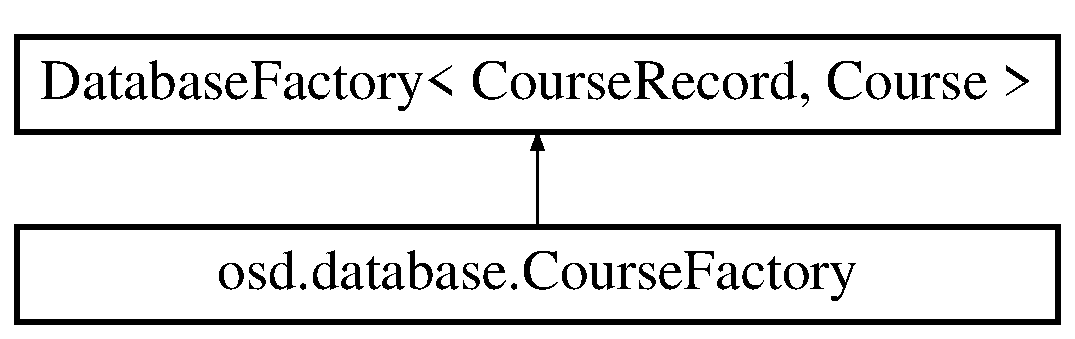
\includegraphics[height=2.000000cm]{classosd_1_1database_1_1_course_factory}
\end{center}
\end{figure}
\subsection*{Public Member Functions}
\begin{DoxyCompactItemize}
\item 
\hypertarget{classosd_1_1database_1_1_course_factory_aac6f17a0a0a2c5ede476c52c1f775a90}{\hyperlink{interfaceosd_1_1input_1_1_course}{Course} {\bfseries create} (final \hyperlink{classosd_1_1database_1_1_course_record}{Course\-Record} record)}\label{classosd_1_1database_1_1_course_factory_aac6f17a0a0a2c5ede476c52c1f775a90}

\end{DoxyCompactItemize}


The documentation for this class was generated from the following file\-:\begin{DoxyCompactItemize}
\item 
/home/travis/build/\-Open-\/\-Source-\/\-Software-\/\-Development/class-\/scheduler/java/src/main/java/osd/database/Course\-Factory.\-java\end{DoxyCompactItemize}

\hypertarget{classosd_1_1database_1_1_course_record}{\section{osd.\-database.\-Course\-Record Class Reference}
\label{classosd_1_1database_1_1_course_record}\index{osd.\-database.\-Course\-Record@{osd.\-database.\-Course\-Record}}
}


The documentation for this class was generated from the following file\-:\begin{DoxyCompactItemize}
\item 
/home/travis/build/\-Open-\/\-Source-\/\-Software-\/\-Development/class-\/scheduler/java/src/main/java/osd/database/Course\-Record.\-java\end{DoxyCompactItemize}

\hypertarget{classosd_1_1database_1_1_database_module}{\section{osd.\-database.\-Database\-Module Class Reference}
\label{classosd_1_1database_1_1_database_module}\index{osd.\-database.\-Database\-Module@{osd.\-database.\-Database\-Module}}
}


The documentation for this class was generated from the following file\-:\begin{DoxyCompactItemize}
\item 
/home/travis/build/\-Open-\/\-Source-\/\-Software-\/\-Development/class-\/scheduler/java/src/main/java/osd/database/Database\-Module.\-java\end{DoxyCompactItemize}

\hypertarget{classscheduler_1_1models_1_1_division}{\section{scheduler.\-models.\-Division Class Reference}
\label{classscheduler_1_1models_1_1_division}\index{scheduler.\-models.\-Division@{scheduler.\-models.\-Division}}
}
Inheritance diagram for scheduler.\-models.\-Division\-:\begin{figure}[H]
\begin{center}
\leavevmode
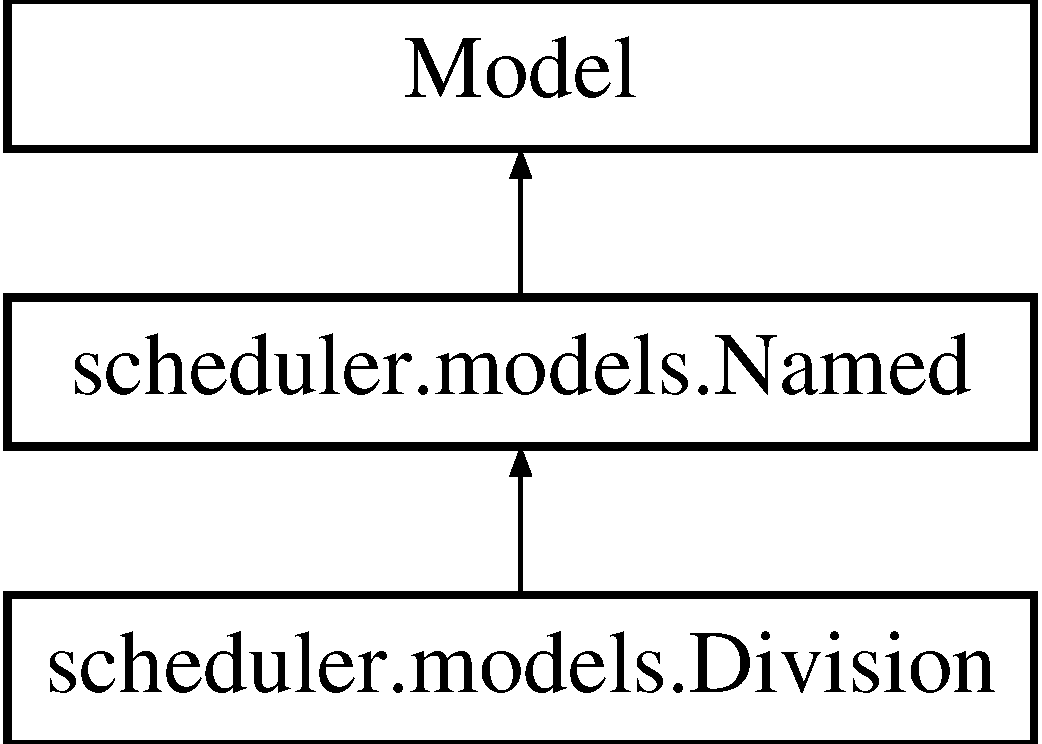
\includegraphics[height=3.000000cm]{classscheduler_1_1models_1_1_division}
\end{center}
\end{figure}
\subsection*{Additional Inherited Members}


\subsection{Detailed Description}
\begin{DoxyVerb}    Table: Division
    Primary Key: Autogenerated identifier.
    Columns: 
        division: CharField (Max Length: 20)
            - This should be all of the division identifiers (ex: ITS)
\end{DoxyVerb}
 

The documentation for this class was generated from the following file\-:\begin{DoxyCompactItemize}
\item 
/home/travis/build/\-Open-\/\-Source-\/\-Software-\/\-Development/class-\/scheduler/mysite/scheduler/models.\-py\end{DoxyCompactItemize}

\hypertarget{classfaculty__data_1_1models_1_1_faculty}{\section{faculty\-\_\-data.\-models.\-Faculty Class Reference}
\label{classfaculty__data_1_1models_1_1_faculty}\index{faculty\-\_\-data.\-models.\-Faculty@{faculty\-\_\-data.\-models.\-Faculty}}
}
Inheritance diagram for faculty\-\_\-data.\-models.\-Faculty\-:\begin{figure}[H]
\begin{center}
\leavevmode
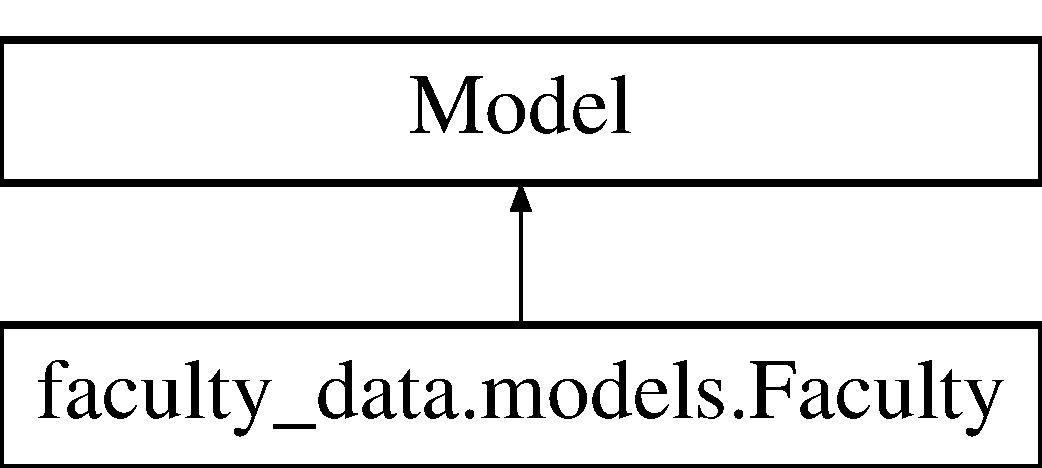
\includegraphics[height=2.000000cm]{classfaculty__data_1_1models_1_1_faculty}
\end{center}
\end{figure}
\subsection*{Public Member Functions}
\begin{DoxyCompactItemize}
\item 
\hypertarget{classfaculty__data_1_1models_1_1_faculty_a5441473cdbd137a5d97eaeee446ff2f8}{def {\bfseries \-\_\-\-\_\-str\-\_\-\-\_\-}}\label{classfaculty__data_1_1models_1_1_faculty_a5441473cdbd137a5d97eaeee446ff2f8}

\end{DoxyCompactItemize}
\subsection*{Static Public Attributes}
\begin{DoxyCompactItemize}
\item 
\hypertarget{classfaculty__data_1_1models_1_1_faculty_a162057cc95e31e5f1db6cf628bcd9be7}{tuple {\bfseries division} = models.\-Char\-Field(max\-\_\-length=20)}\label{classfaculty__data_1_1models_1_1_faculty_a162057cc95e31e5f1db6cf628bcd9be7}

\item 
\hypertarget{classfaculty__data_1_1models_1_1_faculty_a5fefec5b0832df4ffcf413dd83a3280e}{tuple {\bfseries first\-\_\-name} = models.\-Char\-Field(max\-\_\-length=200)}\label{classfaculty__data_1_1models_1_1_faculty_a5fefec5b0832df4ffcf413dd83a3280e}

\item 
\hypertarget{classfaculty__data_1_1models_1_1_faculty_acb398c50a259ddfa78fb96193f0bc177}{tuple {\bfseries last\-\_\-name} = models.\-Char\-Field(max\-\_\-length=200)}\label{classfaculty__data_1_1models_1_1_faculty_acb398c50a259ddfa78fb96193f0bc177}

\item 
\hypertarget{classfaculty__data_1_1models_1_1_faculty_a31c54101010c9cae133a5ab312e30bbd}{tuple {\bfseries subject} = models.\-Char\-Field(max\-\_\-length=200)}\label{classfaculty__data_1_1models_1_1_faculty_a31c54101010c9cae133a5ab312e30bbd}

\item 
\hypertarget{classfaculty__data_1_1models_1_1_faculty_a34c4bea60edfec2bda42d5fdf984fad6}{tuple {\bfseries course} = models.\-Char\-Field(max\-\_\-length=200)}\label{classfaculty__data_1_1models_1_1_faculty_a34c4bea60edfec2bda42d5fdf984fad6}

\end{DoxyCompactItemize}


The documentation for this class was generated from the following file\-:\begin{DoxyCompactItemize}
\item 
/home/travis/build/\-Open-\/\-Source-\/\-Software-\/\-Development/class-\/scheduler/mysite/faculty\-\_\-data/models.\-py\end{DoxyCompactItemize}

\hypertarget{classfaculty__data_1_1apps_1_1_faculty_data_config}{\section{faculty\-\_\-data.\-apps.\-Faculty\-Data\-Config Class Reference}
\label{classfaculty__data_1_1apps_1_1_faculty_data_config}\index{faculty\-\_\-data.\-apps.\-Faculty\-Data\-Config@{faculty\-\_\-data.\-apps.\-Faculty\-Data\-Config}}
}
Inheritance diagram for faculty\-\_\-data.\-apps.\-Faculty\-Data\-Config\-:\begin{figure}[H]
\begin{center}
\leavevmode
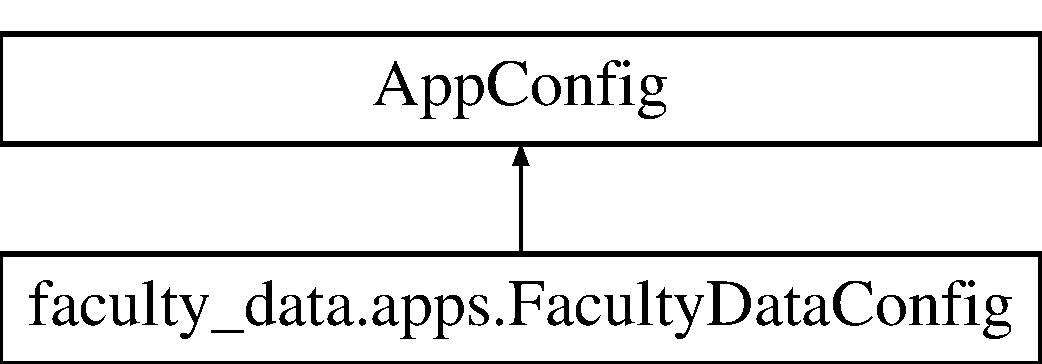
\includegraphics[height=2.000000cm]{classfaculty__data_1_1apps_1_1_faculty_data_config}
\end{center}
\end{figure}
\subsection*{Static Public Attributes}
\begin{DoxyCompactItemize}
\item 
\hypertarget{classfaculty__data_1_1apps_1_1_faculty_data_config_a430bbb7f477ea75ba557a828da2d48ac}{string {\bfseries name} = 'faculty\-\_\-data'}\label{classfaculty__data_1_1apps_1_1_faculty_data_config_a430bbb7f477ea75ba557a828da2d48ac}

\end{DoxyCompactItemize}


The documentation for this class was generated from the following file\-:\begin{DoxyCompactItemize}
\item 
/home/travis/build/\-Open-\/\-Source-\/\-Software-\/\-Development/class-\/scheduler/mysite/faculty\-\_\-data/apps.\-py\end{DoxyCompactItemize}

\hypertarget{classosd_1_1main_1_1_flag_module}{\section{osd.\-main.\-Flag\-Module Class Reference}
\label{classosd_1_1main_1_1_flag_module}\index{osd.\-main.\-Flag\-Module@{osd.\-main.\-Flag\-Module}}
}
\subsection*{Public Member Functions}
\begin{DoxyCompactItemize}
\item 
\hypertarget{classosd_1_1main_1_1_flag_module_a131cd0883177a835b1766f4d4655bb87}{{\bfseries Flag\-Module} (final String\mbox{[}$\,$\mbox{]} args)  throws Parse\-Exception }\label{classosd_1_1main_1_1_flag_module_a131cd0883177a835b1766f4d4655bb87}

\end{DoxyCompactItemize}


The documentation for this class was generated from the following file\-:\begin{DoxyCompactItemize}
\item 
/home/travis/build/\-Open-\/\-Source-\/\-Software-\/\-Development/class-\/scheduler/java/src/main/java/osd/main/Flag\-Module.\-java\end{DoxyCompactItemize}

\hypertarget{classosd_1_1main_1_1_flags}{\section{osd.\-main.\-Flags Class Reference}
\label{classosd_1_1main_1_1_flags}\index{osd.\-main.\-Flags@{osd.\-main.\-Flags}}
}
\subsection*{Public Member Functions}
\begin{DoxyCompactItemize}
\item 
\hypertarget{classosd_1_1main_1_1_flags_a517087945781310a1267c2da33ef0c31}{String {\bfseries get\-Database\-Host} ()}\label{classosd_1_1main_1_1_flags_a517087945781310a1267c2da33ef0c31}

\item 
\hypertarget{classosd_1_1main_1_1_flags_ac19cf26540770eb693fc6dc2b01162cb}{String {\bfseries get\-Database\-Name} ()}\label{classosd_1_1main_1_1_flags_ac19cf26540770eb693fc6dc2b01162cb}

\item 
\hypertarget{classosd_1_1main_1_1_flags_a97f2cbb968226db020be728142e1adb0}{String {\bfseries get\-Database\-User} ()}\label{classosd_1_1main_1_1_flags_a97f2cbb968226db020be728142e1adb0}

\item 
\hypertarget{classosd_1_1main_1_1_flags_a699ec59399c7291817422381a54f116b}{String {\bfseries get\-Database\-Pass} ()}\label{classosd_1_1main_1_1_flags_a699ec59399c7291817422381a54f116b}

\end{DoxyCompactItemize}


The documentation for this class was generated from the following file\-:\begin{DoxyCompactItemize}
\item 
/home/travis/build/\-Open-\/\-Source-\/\-Software-\/\-Development/class-\/scheduler/java/src/main/java/osd/main/Flags.\-java\end{DoxyCompactItemize}

\hypertarget{interfaceosd_1_1input_1_1placeholder_1_1_placeholder_1_1_from_c_s_v}{\section{osd.\-input.\-placeholder.\-Placeholder.\-From\-C\-S\-V Interface Reference}
\label{interfaceosd_1_1input_1_1placeholder_1_1_placeholder_1_1_from_c_s_v}\index{osd.\-input.\-placeholder.\-Placeholder.\-From\-C\-S\-V@{osd.\-input.\-placeholder.\-Placeholder.\-From\-C\-S\-V}}
}
\subsection*{Public Member Functions}
\begin{DoxyCompactItemize}
\item 
\hypertarget{interfaceosd_1_1input_1_1placeholder_1_1_placeholder_1_1_from_c_s_v_a01eadbd76109de58aab6f1b9c3844db4}{int {\bfseries value} ()}\label{interfaceosd_1_1input_1_1placeholder_1_1_placeholder_1_1_from_c_s_v_a01eadbd76109de58aab6f1b9c3844db4}

\end{DoxyCompactItemize}


The documentation for this interface was generated from the following file\-:\begin{DoxyCompactItemize}
\item 
/home/travis/build/\-Open-\/\-Source-\/\-Software-\/\-Development/class-\/scheduler/java/src/main/java/osd/input/placeholder/Placeholder.\-java\end{DoxyCompactItemize}

\hypertarget{classosd_1_1output_1_1_hunk}{\section{osd.\-output.\-Hunk Class Reference}
\label{classosd_1_1output_1_1_hunk}\index{osd.\-output.\-Hunk@{osd.\-output.\-Hunk}}
}
\subsection*{Public Member Functions}
\begin{DoxyCompactItemize}
\item 
\hypertarget{classosd_1_1output_1_1_hunk_a2afad4ffedd8f198524b9890243dc1c9}{{\bfseries Hunk} (final \hyperlink{interfaceosd_1_1input_1_1_section}{Section} section, final \hyperlink{interfaceosd_1_1input_1_1_professor}{Professor} professor, final \hyperlink{interfaceosd_1_1input_1_1_room}{Room} room, final \hyperlink{interfaceosd_1_1input_1_1_block}{Block} block)}\label{classosd_1_1output_1_1_hunk_a2afad4ffedd8f198524b9890243dc1c9}

\item 
\hyperlink{interfaceosd_1_1input_1_1_section}{Section} \hyperlink{classosd_1_1output_1_1_hunk_a4ae048a129a226f5e0f90d42a1fb9070}{get\-Section} ()
\item 
\hyperlink{interfaceosd_1_1input_1_1_professor}{Professor} \hyperlink{classosd_1_1output_1_1_hunk_aad86f22e8a5009d281d3a3ca0bf0f823}{get\-Professor} ()
\item 
\hyperlink{interfaceosd_1_1input_1_1_room}{Room} \hyperlink{classosd_1_1output_1_1_hunk_aec452e382d14f30e6da72e63e647eae3}{get\-Room} ()
\item 
\hyperlink{interfaceosd_1_1input_1_1_block}{Block} \hyperlink{classosd_1_1output_1_1_hunk_a58a55628703e1f9ac88f14f0cbf09bcb}{get\-Block} ()
\item 
\hypertarget{classosd_1_1output_1_1_hunk_a843591462a1402c08cb41c2c598c1ad7}{boolean {\bfseries equals} (final Object o)}\label{classosd_1_1output_1_1_hunk_a843591462a1402c08cb41c2c598c1ad7}

\item 
\hypertarget{classosd_1_1output_1_1_hunk_add37c82837cda95f356962de06d0c8eb}{int {\bfseries hash\-Code} ()}\label{classosd_1_1output_1_1_hunk_add37c82837cda95f356962de06d0c8eb}

\item 
\hypertarget{classosd_1_1output_1_1_hunk_a5d3057c83b319668ddee8a9dcd7204f3}{String {\bfseries to\-String} ()}\label{classosd_1_1output_1_1_hunk_a5d3057c83b319668ddee8a9dcd7204f3}

\item 
\hypertarget{classosd_1_1output_1_1_hunk_a15b10a7f8b23e9e29355e125ca12ee3a}{{\bfseries Hunk} (final \hyperlink{interfaceosd_1_1input_1_1_block}{Block} block, final \hyperlink{interfaceosd_1_1input_1_1_room}{Room} room, final \hyperlink{interfaceosd_1_1input_1_1_professor}{Professor} professor, final \hyperlink{interfaceosd_1_1input_1_1_section}{Section} section)}\label{classosd_1_1output_1_1_hunk_a15b10a7f8b23e9e29355e125ca12ee3a}

\item 
\hypertarget{classosd_1_1output_1_1_hunk_a58a55628703e1f9ac88f14f0cbf09bcb}{\hyperlink{interfaceosd_1_1input_1_1_block}{Block} {\bfseries get\-Block} ()}\label{classosd_1_1output_1_1_hunk_a58a55628703e1f9ac88f14f0cbf09bcb}

\item 
\hypertarget{classosd_1_1output_1_1_hunk_aec452e382d14f30e6da72e63e647eae3}{\hyperlink{interfaceosd_1_1input_1_1_room}{Room} {\bfseries get\-Room} ()}\label{classosd_1_1output_1_1_hunk_aec452e382d14f30e6da72e63e647eae3}

\item 
\hypertarget{classosd_1_1output_1_1_hunk_aad86f22e8a5009d281d3a3ca0bf0f823}{\hyperlink{interfaceosd_1_1input_1_1_professor}{Professor} {\bfseries get\-Professor} ()}\label{classosd_1_1output_1_1_hunk_aad86f22e8a5009d281d3a3ca0bf0f823}

\item 
\hypertarget{classosd_1_1output_1_1_hunk_a4ae048a129a226f5e0f90d42a1fb9070}{\hyperlink{interfaceosd_1_1input_1_1_section}{Section} {\bfseries get\-Section} ()}\label{classosd_1_1output_1_1_hunk_a4ae048a129a226f5e0f90d42a1fb9070}

\item 
\hypertarget{classosd_1_1output_1_1_hunk_add37c82837cda95f356962de06d0c8eb}{int {\bfseries hash\-Code} ()}\label{classosd_1_1output_1_1_hunk_add37c82837cda95f356962de06d0c8eb}

\item 
\hypertarget{classosd_1_1output_1_1_hunk_a843591462a1402c08cb41c2c598c1ad7}{boolean {\bfseries equals} (final Object o)}\label{classosd_1_1output_1_1_hunk_a843591462a1402c08cb41c2c598c1ad7}

\item 
\hypertarget{classosd_1_1output_1_1_hunk_a5d3057c83b319668ddee8a9dcd7204f3}{String {\bfseries to\-String} ()}\label{classosd_1_1output_1_1_hunk_a5d3057c83b319668ddee8a9dcd7204f3}

\end{DoxyCompactItemize}


\subsection{Detailed Description}
Represents a single scheduler output. A hunk is defined by a 
\begin{DoxyCode}
(Section, Professor, Room, Block 
\end{DoxyCode}
 ) 4-\/tuple. This is sufficient to provide all scheduling data needed for the specified section. 

\subsection{Member Function Documentation}
\hypertarget{classosd_1_1output_1_1_hunk_a58a55628703e1f9ac88f14f0cbf09bcb}{\index{osd\-::output\-::\-Hunk@{osd\-::output\-::\-Hunk}!get\-Block@{get\-Block}}
\index{get\-Block@{get\-Block}!osd::output::Hunk@{osd\-::output\-::\-Hunk}}
\subsubsection[{get\-Block}]{\setlength{\rightskip}{0pt plus 5cm}{\bf Block} osd.\-output.\-Hunk.\-get\-Block (
\begin{DoxyParamCaption}
{}
\end{DoxyParamCaption}
)\hspace{0.3cm}{\ttfamily [inline]}}}\label{classosd_1_1output_1_1_hunk_a58a55628703e1f9ac88f14f0cbf09bcb}
Gets the time block the  \hyperlink{classosd_1_1output_1_1_hunk_a4ae048a129a226f5e0f90d42a1fb9070}{get\-Section()} section\} is scheduled at. \begin{DoxyReturn}{Returns}
the time block the section is scheduled at 
\end{DoxyReturn}
\hypertarget{classosd_1_1output_1_1_hunk_aad86f22e8a5009d281d3a3ca0bf0f823}{\index{osd\-::output\-::\-Hunk@{osd\-::output\-::\-Hunk}!get\-Professor@{get\-Professor}}
\index{get\-Professor@{get\-Professor}!osd::output::Hunk@{osd\-::output\-::\-Hunk}}
\subsubsection[{get\-Professor}]{\setlength{\rightskip}{0pt plus 5cm}{\bf Professor} osd.\-output.\-Hunk.\-get\-Professor (
\begin{DoxyParamCaption}
{}
\end{DoxyParamCaption}
)\hspace{0.3cm}{\ttfamily [inline]}}}\label{classosd_1_1output_1_1_hunk_aad86f22e8a5009d281d3a3ca0bf0f823}
Gets the professor slated to teach the  \hyperlink{classosd_1_1output_1_1_hunk_a4ae048a129a226f5e0f90d42a1fb9070}{get\-Section()} section\}. \begin{DoxyReturn}{Returns}
the professor slated to teach the section 
\end{DoxyReturn}
\hypertarget{classosd_1_1output_1_1_hunk_aec452e382d14f30e6da72e63e647eae3}{\index{osd\-::output\-::\-Hunk@{osd\-::output\-::\-Hunk}!get\-Room@{get\-Room}}
\index{get\-Room@{get\-Room}!osd::output::Hunk@{osd\-::output\-::\-Hunk}}
\subsubsection[{get\-Room}]{\setlength{\rightskip}{0pt plus 5cm}{\bf Room} osd.\-output.\-Hunk.\-get\-Room (
\begin{DoxyParamCaption}
{}
\end{DoxyParamCaption}
)\hspace{0.3cm}{\ttfamily [inline]}}}\label{classosd_1_1output_1_1_hunk_aec452e382d14f30e6da72e63e647eae3}
Gets the room the  \hyperlink{classosd_1_1output_1_1_hunk_a4ae048a129a226f5e0f90d42a1fb9070}{get\-Section()} section\} is scheduled at. \begin{DoxyReturn}{Returns}
the room the section is scheduled at 
\end{DoxyReturn}
\hypertarget{classosd_1_1output_1_1_hunk_a4ae048a129a226f5e0f90d42a1fb9070}{\index{osd\-::output\-::\-Hunk@{osd\-::output\-::\-Hunk}!get\-Section@{get\-Section}}
\index{get\-Section@{get\-Section}!osd::output::Hunk@{osd\-::output\-::\-Hunk}}
\subsubsection[{get\-Section}]{\setlength{\rightskip}{0pt plus 5cm}{\bf Section} osd.\-output.\-Hunk.\-get\-Section (
\begin{DoxyParamCaption}
{}
\end{DoxyParamCaption}
)\hspace{0.3cm}{\ttfamily [inline]}}}\label{classosd_1_1output_1_1_hunk_a4ae048a129a226f5e0f90d42a1fb9070}
Gets the course section this hunk provides scheduling data for. \begin{DoxyReturn}{Returns}
the course section this hunk provides scheduling data for 
\end{DoxyReturn}


The documentation for this class was generated from the following file\-:\begin{DoxyCompactItemize}
\item 
/home/travis/build/\-Open-\/\-Source-\/\-Software-\/\-Development/class-\/scheduler/java/src/main/java/osd/output/Hunk.\-java\end{DoxyCompactItemize}

\hypertarget{classscheduler_1_1models_1_1_hunk}{\section{scheduler.\-models.\-Hunk Class Reference}
\label{classscheduler_1_1models_1_1_hunk}\index{scheduler.\-models.\-Hunk@{scheduler.\-models.\-Hunk}}
}
Inheritance diagram for scheduler.\-models.\-Hunk\-:\begin{figure}[H]
\begin{center}
\leavevmode
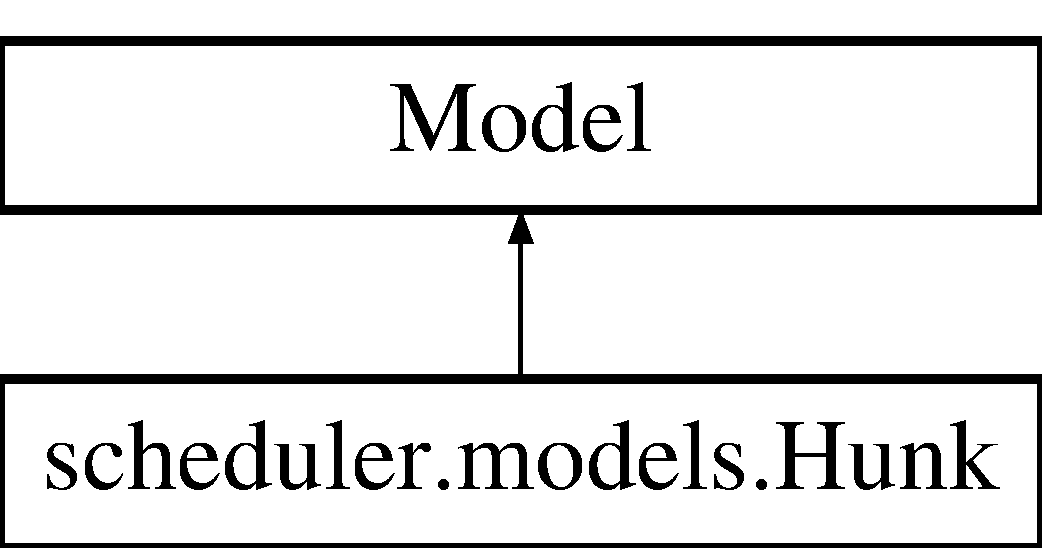
\includegraphics[height=2.000000cm]{classscheduler_1_1models_1_1_hunk}
\end{center}
\end{figure}
\subsection*{Public Member Functions}
\begin{DoxyCompactItemize}
\item 
\hypertarget{classscheduler_1_1models_1_1_hunk_a0ea2e3fef6321aa3e738390c537defde}{def {\bfseries \-\_\-\-\_\-str\-\_\-\-\_\-}}\label{classscheduler_1_1models_1_1_hunk_a0ea2e3fef6321aa3e738390c537defde}

\end{DoxyCompactItemize}
\subsection*{Static Public Attributes}
\begin{DoxyCompactItemize}
\item 
\hypertarget{classscheduler_1_1models_1_1_hunk_a24e5838d535817f4d0cb27f8fb6edd36}{tuple {\bfseries section} = models.\-Foreign\-Key(\hyperlink{classscheduler_1_1models_1_1_section}{Section}, on\-\_\-delete=models.\-C\-A\-S\-C\-A\-D\-E)}\label{classscheduler_1_1models_1_1_hunk_a24e5838d535817f4d0cb27f8fb6edd36}

\item 
\hypertarget{classscheduler_1_1models_1_1_hunk_aa01e29b62d649ce7cd0ccc0e35b51747}{tuple {\bfseries professor} = models.\-Foreign\-Key(\hyperlink{classscheduler_1_1models_1_1_professor}{Professor}, on\-\_\-delete=models.\-C\-A\-S\-C\-A\-D\-E)}\label{classscheduler_1_1models_1_1_hunk_aa01e29b62d649ce7cd0ccc0e35b51747}

\item 
\hypertarget{classscheduler_1_1models_1_1_hunk_ac50c8aaab3e58e9bf1ff953f4246f21a}{tuple {\bfseries room} = models.\-Foreign\-Key(\hyperlink{classscheduler_1_1models_1_1_room}{Room}, on\-\_\-delete=models.\-C\-A\-S\-C\-A\-D\-E)}\label{classscheduler_1_1models_1_1_hunk_ac50c8aaab3e58e9bf1ff953f4246f21a}

\item 
\hypertarget{classscheduler_1_1models_1_1_hunk_ab6e2df449de158fcf00218f6f2e63832}{tuple {\bfseries block} = models.\-Foreign\-Key(\hyperlink{classscheduler_1_1models_1_1_block}{Block}, on\-\_\-delete=models.\-C\-A\-S\-C\-A\-D\-E)}\label{classscheduler_1_1models_1_1_hunk_ab6e2df449de158fcf00218f6f2e63832}

\end{DoxyCompactItemize}


\subsection{Detailed Description}
\begin{DoxyVerb}    TODO:
        Documentation
\end{DoxyVerb}
 

The documentation for this class was generated from the following file\-:\begin{DoxyCompactItemize}
\item 
/home/travis/build/\-Open-\/\-Source-\/\-Software-\/\-Development/class-\/scheduler/mysite/scheduler/models.\-py\end{DoxyCompactItemize}

\hypertarget{classosd_1_1input_1_1_input_module}{\section{osd.\-input.\-Input\-Module Class Reference}
\label{classosd_1_1input_1_1_input_module}\index{osd.\-input.\-Input\-Module@{osd.\-input.\-Input\-Module}}
}
\subsection*{Classes}
\begin{DoxyCompactItemize}
\item 
interface \hyperlink{interfaceosd_1_1input_1_1_input_module_1_1_sources_module}{Sources\-Module}
\end{DoxyCompactItemize}


The documentation for this class was generated from the following file\-:\begin{DoxyCompactItemize}
\item 
/home/travis/build/\-Open-\/\-Source-\/\-Software-\/\-Development/class-\/scheduler/java/src/main/java/osd/input/Input\-Module.\-java\end{DoxyCompactItemize}

\hypertarget{interfaceosd_1_1considerations_1_1_lookups}{\section{osd.\-considerations.\-Lookups Interface Reference}
\label{interfaceosd_1_1considerations_1_1_lookups}\index{osd.\-considerations.\-Lookups@{osd.\-considerations.\-Lookups}}
}


Inherited by osd.\-schedule.\-Scheduler\-Lookups.

\subsection*{Public Member Functions}
\begin{DoxyCompactItemize}
\item 
\hypertarget{interfaceosd_1_1considerations_1_1_lookups_a79f815304368deb1c52f7aacb1f7a82a}{Stream$<$ \hyperlink{classosd_1_1output_1_1_hunk}{Hunk} $>$ {\bfseries lookup\-All\-Hunks} ()}\label{interfaceosd_1_1considerations_1_1_lookups_a79f815304368deb1c52f7aacb1f7a82a}

\item 
Stream$<$ \hyperlink{classosd_1_1output_1_1_hunk}{Hunk} $>$ \hyperlink{interfaceosd_1_1considerations_1_1_lookups_a59cce51ecd4a4d7759d75fe22764618e}{lookup} (\hyperlink{interfaceosd_1_1input_1_1_professor}{Professor} professor)
\item 
Stream$<$ \hyperlink{classosd_1_1output_1_1_hunk}{Hunk} $>$ \hyperlink{interfaceosd_1_1considerations_1_1_lookups_a3555d841515dc41635a5630b9fb9d2db}{lookup} (\hyperlink{interfaceosd_1_1input_1_1_block}{Block} block)
\item 
\hyperlink{classosd_1_1output_1_1_hunk}{Hunk} \hyperlink{interfaceosd_1_1considerations_1_1_lookups_a887396578bd66cac95589f68cfc2d50f}{lookup} (\hyperlink{interfaceosd_1_1input_1_1_section}{Section} section)
\end{DoxyCompactItemize}


\subsection{Detailed Description}
Additional information available to base constraints and base preferences. 

\subsection{Member Function Documentation}
\hypertarget{interfaceosd_1_1considerations_1_1_lookups_a59cce51ecd4a4d7759d75fe22764618e}{\index{osd\-::considerations\-::\-Lookups@{osd\-::considerations\-::\-Lookups}!lookup@{lookup}}
\index{lookup@{lookup}!osd::considerations::Lookups@{osd\-::considerations\-::\-Lookups}}
\subsubsection[{lookup}]{\setlength{\rightskip}{0pt plus 5cm}Stream$<${\bf Hunk}$>$ osd.\-considerations.\-Lookups.\-lookup (
\begin{DoxyParamCaption}
\item[{{\bf Professor}}]{professor}
\end{DoxyParamCaption}
)}}\label{interfaceosd_1_1considerations_1_1_lookups_a59cce51ecd4a4d7759d75fe22764618e}
Get all the hunks for which a professor is scheduled. If the professor has not yet been scheduled anywhere, return an empty stream. 
\begin{DoxyParams}{Parameters}
{\em professor} & the professor to look up hunks for \\
\hline
\end{DoxyParams}
\begin{DoxyReturn}{Returns}
a (possibly empty, non-\/null) hunk stream for that professor 
\end{DoxyReturn}
\hypertarget{interfaceosd_1_1considerations_1_1_lookups_a3555d841515dc41635a5630b9fb9d2db}{\index{osd\-::considerations\-::\-Lookups@{osd\-::considerations\-::\-Lookups}!lookup@{lookup}}
\index{lookup@{lookup}!osd::considerations::Lookups@{osd\-::considerations\-::\-Lookups}}
\subsubsection[{lookup}]{\setlength{\rightskip}{0pt plus 5cm}Stream$<${\bf Hunk}$>$ osd.\-considerations.\-Lookups.\-lookup (
\begin{DoxyParamCaption}
\item[{{\bf Block}}]{block}
\end{DoxyParamCaption}
)}}\label{interfaceosd_1_1considerations_1_1_lookups_a3555d841515dc41635a5630b9fb9d2db}
Get all the hunks during a certain block. If no hunks have yet been scheduled at that block, return and empty stream. 
\begin{DoxyParams}{Parameters}
{\em block} & the block to look up hunks for \\
\hline
\end{DoxyParams}
\begin{DoxyReturn}{Returns}
a (possibly empty, non-\/null) hunk stream for that professor 
\end{DoxyReturn}
\hypertarget{interfaceosd_1_1considerations_1_1_lookups_a887396578bd66cac95589f68cfc2d50f}{\index{osd\-::considerations\-::\-Lookups@{osd\-::considerations\-::\-Lookups}!lookup@{lookup}}
\index{lookup@{lookup}!osd::considerations::Lookups@{osd\-::considerations\-::\-Lookups}}
\subsubsection[{lookup}]{\setlength{\rightskip}{0pt plus 5cm}{\bf Hunk} osd.\-considerations.\-Lookups.\-lookup (
\begin{DoxyParamCaption}
\item[{{\bf Section}}]{section}
\end{DoxyParamCaption}
)}}\label{interfaceosd_1_1considerations_1_1_lookups_a887396578bd66cac95589f68cfc2d50f}
Find the hunk for a section. If the section has not been scheduled yet, return
\begin{DoxyCode}
null 
\end{DoxyCode}
 . 
\begin{DoxyParams}{Parameters}
{\em section} & the section to look up a hunk for \\
\hline
\end{DoxyParams}
\begin{DoxyReturn}{Returns}
the (possibly null) hunk for that section 
\end{DoxyReturn}


The documentation for this interface was generated from the following file\-:\begin{DoxyCompactItemize}
\item 
/home/travis/build/\-Open-\/\-Source-\/\-Software-\/\-Development/class-\/scheduler/java/src/main/java/osd/considerations/Lookups.\-java\end{DoxyCompactItemize}

\hypertarget{classosd_1_1util_1_1relation_1_1_many_to_many_relation_3_01_k_00_01_v_01_4}{\section{osd.\-util.\-relation.\-Many\-To\-Many\-Relation$<$ K, V $>$ Class Reference}
\label{classosd_1_1util_1_1relation_1_1_many_to_many_relation_3_01_k_00_01_v_01_4}\index{osd.\-util.\-relation.\-Many\-To\-Many\-Relation$<$ K, V $>$@{osd.\-util.\-relation.\-Many\-To\-Many\-Relation$<$ K, V $>$}}
}
Inheritance diagram for osd.\-util.\-relation.\-Many\-To\-Many\-Relation$<$ K, V $>$\-:\begin{figure}[H]
\begin{center}
\leavevmode
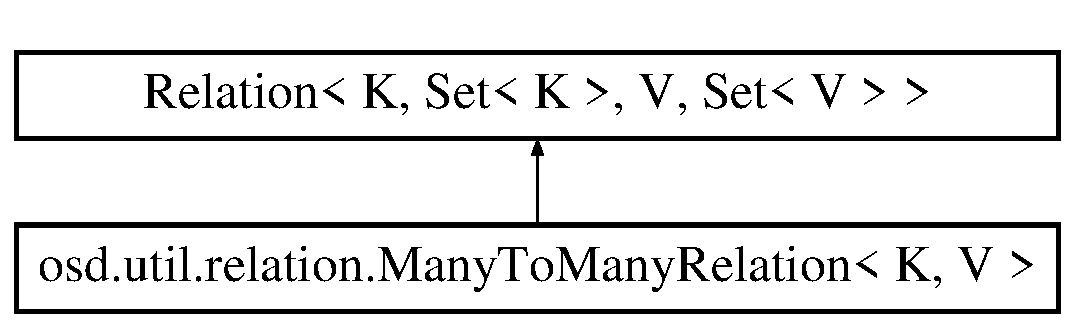
\includegraphics[height=2.000000cm]{classosd_1_1util_1_1relation_1_1_many_to_many_relation_3_01_k_00_01_v_01_4}
\end{center}
\end{figure}
\subsection*{Public Member Functions}
\begin{DoxyCompactItemize}
\item 
\hyperlink{classosd_1_1util_1_1relation_1_1_many_to_many_relation_3_01_k_00_01_v_01_4_a6e2952d72db443443845d52b1a6e4b5b}{Many\-To\-Many\-Relation} ()
\item 
\hyperlink{classosd_1_1util_1_1relation_1_1_many_to_many_relation_3_01_k_00_01_v_01_4_a16dc7bf49e896e39d9f8380ddc3f80b6}{Many\-To\-Many\-Relation} (final Relation$<$ K, Set$<$ K $>$, V, Set$<$ V $>$$>$ copy\-Of)
\item 
\hypertarget{classosd_1_1util_1_1relation_1_1_many_to_many_relation_3_01_k_00_01_v_01_4_a097c72570ffc4b114cccd4124879398f}{void {\bfseries add} (final K key, final V value)}\label{classosd_1_1util_1_1relation_1_1_many_to_many_relation_3_01_k_00_01_v_01_4_a097c72570ffc4b114cccd4124879398f}

\item 
\hypertarget{classosd_1_1util_1_1relation_1_1_many_to_many_relation_3_01_k_00_01_v_01_4_a0eea8c6a44dc7ed9d119b47c173c9d75}{void {\bfseries remove} (final K key, final V value)}\label{classosd_1_1util_1_1relation_1_1_many_to_many_relation_3_01_k_00_01_v_01_4_a0eea8c6a44dc7ed9d119b47c173c9d75}

\item 
\hypertarget{classosd_1_1util_1_1relation_1_1_many_to_many_relation_3_01_k_00_01_v_01_4_ae5eb9dd6957255b13048122b17466001}{void {\bfseries remove} (final K key)}\label{classosd_1_1util_1_1relation_1_1_many_to_many_relation_3_01_k_00_01_v_01_4_ae5eb9dd6957255b13048122b17466001}

\item 
\hypertarget{classosd_1_1util_1_1relation_1_1_many_to_many_relation_3_01_k_00_01_v_01_4_a1bd698b9d8e715e18e243dd8557d4fc1}{\hyperlink{classosd_1_1util_1_1relation_1_1_many_to_many_relation_3_01_k_00_01_v_01_4_a6e2952d72db443443845d52b1a6e4b5b}{Many\-To\-Many\-Relation}$<$ V, K $>$ {\bfseries reversed} ()}\label{classosd_1_1util_1_1relation_1_1_many_to_many_relation_3_01_k_00_01_v_01_4_a1bd698b9d8e715e18e243dd8557d4fc1}

\end{DoxyCompactItemize}
\subsection*{Protected Member Functions}
\begin{DoxyCompactItemize}
\item 
\hyperlink{classosd_1_1util_1_1relation_1_1_many_to_many_relation_3_01_k_00_01_v_01_4_abdf2b187c2f80f266bb0fc5ef2ce43c3}{Many\-To\-Many\-Relation} (final Map$<$ K, Set$<$ V $>$$>$ forward, final Map$<$ V, Set$<$ K $>$$>$ reverse)
\end{DoxyCompactItemize}


\subsection{Constructor \& Destructor Documentation}
\hypertarget{classosd_1_1util_1_1relation_1_1_many_to_many_relation_3_01_k_00_01_v_01_4_a6e2952d72db443443845d52b1a6e4b5b}{\index{osd\-::util\-::relation\-::\-Many\-To\-Many\-Relation$<$ K, V $>$@{osd\-::util\-::relation\-::\-Many\-To\-Many\-Relation$<$ K, V $>$}!Many\-To\-Many\-Relation@{Many\-To\-Many\-Relation}}
\index{Many\-To\-Many\-Relation@{Many\-To\-Many\-Relation}!osd::util::relation::ManyToManyRelation< K, V >@{osd\-::util\-::relation\-::\-Many\-To\-Many\-Relation$<$ K, V $>$}}
\subsubsection[{Many\-To\-Many\-Relation}]{\setlength{\rightskip}{0pt plus 5cm}osd.\-util.\-relation.\-Many\-To\-Many\-Relation$<$ K, V $>$.Many\-To\-Many\-Relation (
\begin{DoxyParamCaption}
{}
\end{DoxyParamCaption}
)\hspace{0.3cm}{\ttfamily [inline]}}}\label{classosd_1_1util_1_1relation_1_1_many_to_many_relation_3_01_k_00_01_v_01_4_a6e2952d72db443443845d52b1a6e4b5b}
Constructs a new relation with no data. \hypertarget{classosd_1_1util_1_1relation_1_1_many_to_many_relation_3_01_k_00_01_v_01_4_a16dc7bf49e896e39d9f8380ddc3f80b6}{\index{osd\-::util\-::relation\-::\-Many\-To\-Many\-Relation$<$ K, V $>$@{osd\-::util\-::relation\-::\-Many\-To\-Many\-Relation$<$ K, V $>$}!Many\-To\-Many\-Relation@{Many\-To\-Many\-Relation}}
\index{Many\-To\-Many\-Relation@{Many\-To\-Many\-Relation}!osd::util::relation::ManyToManyRelation< K, V >@{osd\-::util\-::relation\-::\-Many\-To\-Many\-Relation$<$ K, V $>$}}
\subsubsection[{Many\-To\-Many\-Relation}]{\setlength{\rightskip}{0pt plus 5cm}osd.\-util.\-relation.\-Many\-To\-Many\-Relation$<$ K, V $>$.Many\-To\-Many\-Relation (
\begin{DoxyParamCaption}
\item[{final Relation$<$ K, Set$<$ K $>$, V, Set$<$ V $>$$>$}]{copy\-Of}
\end{DoxyParamCaption}
)\hspace{0.3cm}{\ttfamily [inline]}}}\label{classosd_1_1util_1_1relation_1_1_many_to_many_relation_3_01_k_00_01_v_01_4_a16dc7bf49e896e39d9f8380ddc3f80b6}
Copy constructor. The original relation and the copy are completely separate; changes to one will not be reflected in the other. 
\begin{DoxyParams}{Parameters}
{\em copy\-Of} & the relation to copy \\
\hline
\end{DoxyParams}
\hypertarget{classosd_1_1util_1_1relation_1_1_many_to_many_relation_3_01_k_00_01_v_01_4_abdf2b187c2f80f266bb0fc5ef2ce43c3}{\index{osd\-::util\-::relation\-::\-Many\-To\-Many\-Relation$<$ K, V $>$@{osd\-::util\-::relation\-::\-Many\-To\-Many\-Relation$<$ K, V $>$}!Many\-To\-Many\-Relation@{Many\-To\-Many\-Relation}}
\index{Many\-To\-Many\-Relation@{Many\-To\-Many\-Relation}!osd::util::relation::ManyToManyRelation< K, V >@{osd\-::util\-::relation\-::\-Many\-To\-Many\-Relation$<$ K, V $>$}}
\subsubsection[{Many\-To\-Many\-Relation}]{\setlength{\rightskip}{0pt plus 5cm}osd.\-util.\-relation.\-Many\-To\-Many\-Relation$<$ K, V $>$.Many\-To\-Many\-Relation (
\begin{DoxyParamCaption}
\item[{final Map$<$ K, Set$<$ V $>$$>$}]{forward, }
\item[{final Map$<$ V, Set$<$ K $>$$>$}]{reverse}
\end{DoxyParamCaption}
)\hspace{0.3cm}{\ttfamily [inline]}, {\ttfamily [protected]}}}\label{classosd_1_1util_1_1relation_1_1_many_to_many_relation_3_01_k_00_01_v_01_4_abdf2b187c2f80f266bb0fc5ef2ce43c3}
View constructor. The relation's maps are supplied directly, and it will read and write to them as appropriate. Be careful with this. 
\begin{DoxyParams}{Parameters}
{\em forward} & the forward map \\
\hline
{\em reverse} & the reverse map \\
\hline
\end{DoxyParams}


The documentation for this class was generated from the following file\-:\begin{DoxyCompactItemize}
\item 
/home/travis/build/\-Open-\/\-Source-\/\-Software-\/\-Development/class-\/scheduler/java/src/main/java/osd/util/relation/Many\-To\-Many\-Relation.\-java\end{DoxyCompactItemize}

\hypertarget{classosd_1_1util_1_1relation_1_1_many_to_one_relation_3_01_k_00_01_v_01_4}{\section{osd.\-util.\-relation.\-Many\-To\-One\-Relation$<$ K, V $>$ Class Reference}
\label{classosd_1_1util_1_1relation_1_1_many_to_one_relation_3_01_k_00_01_v_01_4}\index{osd.\-util.\-relation.\-Many\-To\-One\-Relation$<$ K, V $>$@{osd.\-util.\-relation.\-Many\-To\-One\-Relation$<$ K, V $>$}}
}
Inheritance diagram for osd.\-util.\-relation.\-Many\-To\-One\-Relation$<$ K, V $>$\-:\begin{figure}[H]
\begin{center}
\leavevmode
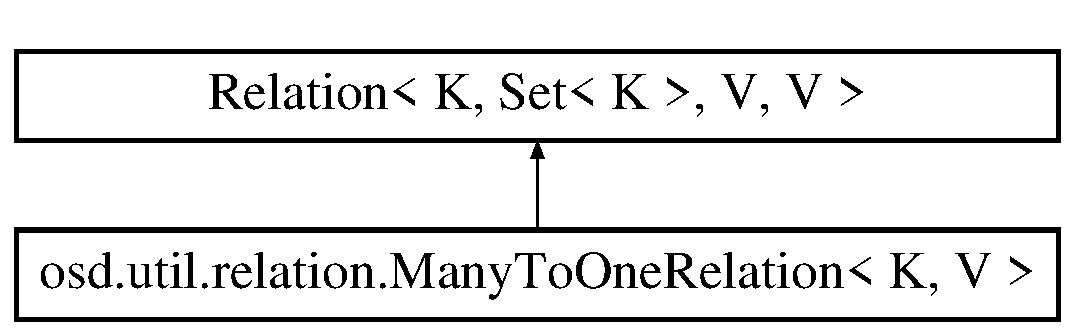
\includegraphics[height=2.000000cm]{classosd_1_1util_1_1relation_1_1_many_to_one_relation_3_01_k_00_01_v_01_4}
\end{center}
\end{figure}
\subsection*{Public Member Functions}
\begin{DoxyCompactItemize}
\item 
\hyperlink{classosd_1_1util_1_1relation_1_1_many_to_one_relation_3_01_k_00_01_v_01_4_ac56d2bc8dd62b1d7ab3036f587198417}{Many\-To\-One\-Relation} ()
\item 
\hyperlink{classosd_1_1util_1_1relation_1_1_many_to_one_relation_3_01_k_00_01_v_01_4_abacd8dc859239fc64cfe911c97bf70a6}{Many\-To\-One\-Relation} (final Relation$<$ K, Set$<$ K $>$, V, V $>$ copy\-Of)
\item 
\hypertarget{classosd_1_1util_1_1relation_1_1_many_to_one_relation_3_01_k_00_01_v_01_4_a6874945591b5971c0aaa5fdda02a5af3}{void {\bfseries add} (final K key, final V value)}\label{classosd_1_1util_1_1relation_1_1_many_to_one_relation_3_01_k_00_01_v_01_4_a6874945591b5971c0aaa5fdda02a5af3}

\item 
\hypertarget{classosd_1_1util_1_1relation_1_1_many_to_one_relation_3_01_k_00_01_v_01_4_a6bd082b03892fa7d2281a407c82c115b}{void {\bfseries remove} (final K key, final V value)}\label{classosd_1_1util_1_1relation_1_1_many_to_one_relation_3_01_k_00_01_v_01_4_a6bd082b03892fa7d2281a407c82c115b}

\item 
\hypertarget{classosd_1_1util_1_1relation_1_1_many_to_one_relation_3_01_k_00_01_v_01_4_acbbdf0c3a1eaa14d1633ee99e64c0d98}{void {\bfseries remove} (final K key)}\label{classosd_1_1util_1_1relation_1_1_many_to_one_relation_3_01_k_00_01_v_01_4_acbbdf0c3a1eaa14d1633ee99e64c0d98}

\item 
\hypertarget{classosd_1_1util_1_1relation_1_1_many_to_one_relation_3_01_k_00_01_v_01_4_aa0a400f0e341ae6693869be1bca6a5f0}{Relation$<$ V, V, K, Set$<$ K $>$ $>$ {\bfseries reversed} ()}\label{classosd_1_1util_1_1relation_1_1_many_to_one_relation_3_01_k_00_01_v_01_4_aa0a400f0e341ae6693869be1bca6a5f0}

\end{DoxyCompactItemize}
\subsection*{Protected Member Functions}
\begin{DoxyCompactItemize}
\item 
\hyperlink{classosd_1_1util_1_1relation_1_1_many_to_one_relation_3_01_k_00_01_v_01_4_a60d0bfe083f2ed97a2084bef8ebf84fd}{Many\-To\-One\-Relation} (final Map$<$ K, V $>$ forward, final Map$<$ V, Set$<$ K $>$$>$ reverse)
\end{DoxyCompactItemize}


\subsection{Constructor \& Destructor Documentation}
\hypertarget{classosd_1_1util_1_1relation_1_1_many_to_one_relation_3_01_k_00_01_v_01_4_ac56d2bc8dd62b1d7ab3036f587198417}{\index{osd\-::util\-::relation\-::\-Many\-To\-One\-Relation$<$ K, V $>$@{osd\-::util\-::relation\-::\-Many\-To\-One\-Relation$<$ K, V $>$}!Many\-To\-One\-Relation@{Many\-To\-One\-Relation}}
\index{Many\-To\-One\-Relation@{Many\-To\-One\-Relation}!osd::util::relation::ManyToOneRelation< K, V >@{osd\-::util\-::relation\-::\-Many\-To\-One\-Relation$<$ K, V $>$}}
\subsubsection[{Many\-To\-One\-Relation}]{\setlength{\rightskip}{0pt plus 5cm}osd.\-util.\-relation.\-Many\-To\-One\-Relation$<$ K, V $>$.Many\-To\-One\-Relation (
\begin{DoxyParamCaption}
{}
\end{DoxyParamCaption}
)\hspace{0.3cm}{\ttfamily [inline]}}}\label{classosd_1_1util_1_1relation_1_1_many_to_one_relation_3_01_k_00_01_v_01_4_ac56d2bc8dd62b1d7ab3036f587198417}
Constructs a new relation with no data. \hypertarget{classosd_1_1util_1_1relation_1_1_many_to_one_relation_3_01_k_00_01_v_01_4_abacd8dc859239fc64cfe911c97bf70a6}{\index{osd\-::util\-::relation\-::\-Many\-To\-One\-Relation$<$ K, V $>$@{osd\-::util\-::relation\-::\-Many\-To\-One\-Relation$<$ K, V $>$}!Many\-To\-One\-Relation@{Many\-To\-One\-Relation}}
\index{Many\-To\-One\-Relation@{Many\-To\-One\-Relation}!osd::util::relation::ManyToOneRelation< K, V >@{osd\-::util\-::relation\-::\-Many\-To\-One\-Relation$<$ K, V $>$}}
\subsubsection[{Many\-To\-One\-Relation}]{\setlength{\rightskip}{0pt plus 5cm}osd.\-util.\-relation.\-Many\-To\-One\-Relation$<$ K, V $>$.Many\-To\-One\-Relation (
\begin{DoxyParamCaption}
\item[{final Relation$<$ K, Set$<$ K $>$, V, V $>$}]{copy\-Of}
\end{DoxyParamCaption}
)\hspace{0.3cm}{\ttfamily [inline]}}}\label{classosd_1_1util_1_1relation_1_1_many_to_one_relation_3_01_k_00_01_v_01_4_abacd8dc859239fc64cfe911c97bf70a6}
Copy constructor. The original relation and the copy are completely separate; changes to one will not be reflected in the other. 
\begin{DoxyParams}{Parameters}
{\em copy\-Of} & the relation to copy \\
\hline
\end{DoxyParams}
\hypertarget{classosd_1_1util_1_1relation_1_1_many_to_one_relation_3_01_k_00_01_v_01_4_a60d0bfe083f2ed97a2084bef8ebf84fd}{\index{osd\-::util\-::relation\-::\-Many\-To\-One\-Relation$<$ K, V $>$@{osd\-::util\-::relation\-::\-Many\-To\-One\-Relation$<$ K, V $>$}!Many\-To\-One\-Relation@{Many\-To\-One\-Relation}}
\index{Many\-To\-One\-Relation@{Many\-To\-One\-Relation}!osd::util::relation::ManyToOneRelation< K, V >@{osd\-::util\-::relation\-::\-Many\-To\-One\-Relation$<$ K, V $>$}}
\subsubsection[{Many\-To\-One\-Relation}]{\setlength{\rightskip}{0pt plus 5cm}osd.\-util.\-relation.\-Many\-To\-One\-Relation$<$ K, V $>$.Many\-To\-One\-Relation (
\begin{DoxyParamCaption}
\item[{final Map$<$ K, V $>$}]{forward, }
\item[{final Map$<$ V, Set$<$ K $>$$>$}]{reverse}
\end{DoxyParamCaption}
)\hspace{0.3cm}{\ttfamily [inline]}, {\ttfamily [protected]}}}\label{classosd_1_1util_1_1relation_1_1_many_to_one_relation_3_01_k_00_01_v_01_4_a60d0bfe083f2ed97a2084bef8ebf84fd}
View constructor. The relation's maps are supplied directly, and it will read and write to them as appropriate. Be careful with this. 
\begin{DoxyParams}{Parameters}
{\em forward} & the forward map \\
\hline
{\em reverse} & the reverse map \\
\hline
\end{DoxyParams}


The documentation for this class was generated from the following file\-:\begin{DoxyCompactItemize}
\item 
/home/travis/build/\-Open-\/\-Source-\/\-Software-\/\-Development/class-\/scheduler/java/src/main/java/osd/util/relation/Many\-To\-One\-Relation.\-java\end{DoxyCompactItemize}

\hypertarget{classscheduler_1_1models_1_1_named_1_1_meta}{\section{scheduler.\-models.\-Named.\-Meta Class Reference}
\label{classscheduler_1_1models_1_1_named_1_1_meta}\index{scheduler.\-models.\-Named.\-Meta@{scheduler.\-models.\-Named.\-Meta}}
}
\subsection*{Static Public Attributes}
\begin{DoxyCompactItemize}
\item 
\hypertarget{classscheduler_1_1models_1_1_named_1_1_meta_a15a08f213947349b70c40da1a57d1e3c}{{\bfseries abstract} = True}\label{classscheduler_1_1models_1_1_named_1_1_meta_a15a08f213947349b70c40da1a57d1e3c}

\end{DoxyCompactItemize}


The documentation for this class was generated from the following file\-:\begin{DoxyCompactItemize}
\item 
/home/travis/build/\-Open-\/\-Source-\/\-Software-\/\-Development/class-\/scheduler/mysite/scheduler/models.\-py\end{DoxyCompactItemize}

\hypertarget{classscheduler_1_1models_1_1_user_preference_or_constraint_1_1_meta}{\section{scheduler.\-models.\-User\-Preference\-Or\-Constraint.\-Meta Class Reference}
\label{classscheduler_1_1models_1_1_user_preference_or_constraint_1_1_meta}\index{scheduler.\-models.\-User\-Preference\-Or\-Constraint.\-Meta@{scheduler.\-models.\-User\-Preference\-Or\-Constraint.\-Meta}}
}
\subsection*{Static Public Attributes}
\begin{DoxyCompactItemize}
\item 
\hypertarget{classscheduler_1_1models_1_1_user_preference_or_constraint_1_1_meta_a96e43107f2412f8afb1c0c2d416d151e}{{\bfseries abstract} = True}\label{classscheduler_1_1models_1_1_user_preference_or_constraint_1_1_meta_a96e43107f2412f8afb1c0c2d416d151e}

\end{DoxyCompactItemize}


The documentation for this class was generated from the following file\-:\begin{DoxyCompactItemize}
\item 
/home/travis/build/\-Open-\/\-Source-\/\-Software-\/\-Development/class-\/scheduler/mysite/scheduler/models.\-py\end{DoxyCompactItemize}

\hypertarget{classfaculty__data_1_1migrations_1_10001__initial_1_1_migration}{\section{faculty\-\_\-data.\-migrations.0001\-\_\-initial.Migration Class Reference}
\label{classfaculty__data_1_1migrations_1_10001__initial_1_1_migration}\index{faculty\-\_\-data.\-migrations.\-0001\-\_\-initial.\-Migration@{faculty\-\_\-data.\-migrations.\-0001\-\_\-initial.\-Migration}}
}
Inheritance diagram for faculty\-\_\-data.\-migrations.0001\-\_\-initial.Migration\-:\begin{figure}[H]
\begin{center}
\leavevmode
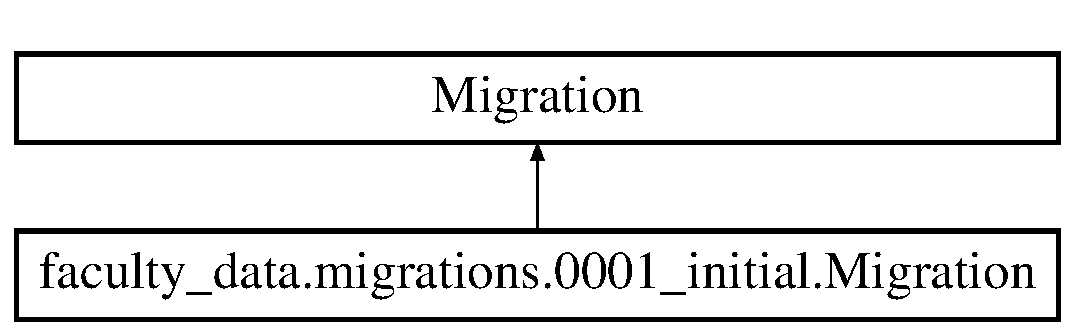
\includegraphics[height=2.000000cm]{classfaculty__data_1_1migrations_1_10001__initial_1_1_migration}
\end{center}
\end{figure}
\subsection*{Static Public Attributes}
\begin{DoxyCompactItemize}
\item 
\hypertarget{classfaculty__data_1_1migrations_1_10001__initial_1_1_migration_a87fa990bdc19b1b865db7693c75b0195}{{\bfseries initial} = True}\label{classfaculty__data_1_1migrations_1_10001__initial_1_1_migration_a87fa990bdc19b1b865db7693c75b0195}

\item 
list {\bfseries dependencies}
\item 
list {\bfseries operations}
\end{DoxyCompactItemize}


\subsection{Member Data Documentation}
\hypertarget{classfaculty__data_1_1migrations_1_10001__initial_1_1_migration_a5b29328b7bc014cdf07fb3793fb187eb}{\index{faculty\-\_\-data\-::migrations\-::0001\-\_\-initial\-::\-Migration@{faculty\-\_\-data\-::migrations\-::0001\-\_\-initial\-::\-Migration}!dependencies@{dependencies}}
\index{dependencies@{dependencies}!faculty_data::migrations::0001_initial::Migration@{faculty\-\_\-data\-::migrations\-::0001\-\_\-initial\-::\-Migration}}
\subsubsection[{dependencies}]{\setlength{\rightskip}{0pt plus 5cm}list faculty\-\_\-data.\-migrations.\-0001\-\_\-initial.\-Migration.\-dependencies\hspace{0.3cm}{\ttfamily [static]}}}\label{classfaculty__data_1_1migrations_1_10001__initial_1_1_migration_a5b29328b7bc014cdf07fb3793fb187eb}
{\bfseries Initial value\-:}
\begin{DoxyCode}
1 = [
2     ]
\end{DoxyCode}
\hypertarget{classfaculty__data_1_1migrations_1_10001__initial_1_1_migration_a3b462f7f278614cec6e12eaf6da24d81}{\index{faculty\-\_\-data\-::migrations\-::0001\-\_\-initial\-::\-Migration@{faculty\-\_\-data\-::migrations\-::0001\-\_\-initial\-::\-Migration}!operations@{operations}}
\index{operations@{operations}!faculty_data::migrations::0001_initial::Migration@{faculty\-\_\-data\-::migrations\-::0001\-\_\-initial\-::\-Migration}}
\subsubsection[{operations}]{\setlength{\rightskip}{0pt plus 5cm}list faculty\-\_\-data.\-migrations.\-0001\-\_\-initial.\-Migration.\-operations\hspace{0.3cm}{\ttfamily [static]}}}\label{classfaculty__data_1_1migrations_1_10001__initial_1_1_migration_a3b462f7f278614cec6e12eaf6da24d81}
{\bfseries Initial value\-:}
\begin{DoxyCode}
1 = [
2         migrations.CreateModel(
3             name=\textcolor{stringliteral}{'Faculty'},
4             fields=[
5                 (\textcolor{stringliteral}{'id'}, models.AutoField(auto\_created=\textcolor{keyword}{True}, primary\_key=\textcolor{keyword}{True}, serialize=\textcolor{keyword}{False}, verbose\_name=\textcolor{stringliteral}{
      'ID'})),
6                 (\textcolor{stringliteral}{'division'}, models.CharField(max\_length=20)),
7                 (\textcolor{stringliteral}{'first\_name'}, models.CharField(max\_length=200)),
8                 (\textcolor{stringliteral}{'last\_name'}, models.CharField(max\_length=200)),
9                 (\textcolor{stringliteral}{'subject'}, models.CharField(max\_length=200)),
10                 (\textcolor{stringliteral}{'course'}, models.CharField(max\_length=200)),
11             ],
12         ),
13     ]
\end{DoxyCode}


The documentation for this class was generated from the following file\-:\begin{DoxyCompactItemize}
\item 
/home/travis/build/\-Open-\/\-Source-\/\-Software-\/\-Development/class-\/scheduler/mysite/faculty\-\_\-data/migrations/0001\-\_\-initial.\-py\end{DoxyCompactItemize}

\hypertarget{classroom__data_1_1migrations_1_10001__initial_1_1_migration}{\section{room\-\_\-data.\-migrations.0001\-\_\-initial.Migration Class Reference}
\label{classroom__data_1_1migrations_1_10001__initial_1_1_migration}\index{room\-\_\-data.\-migrations.\-0001\-\_\-initial.\-Migration@{room\-\_\-data.\-migrations.\-0001\-\_\-initial.\-Migration}}
}
Inheritance diagram for room\-\_\-data.\-migrations.0001\-\_\-initial.Migration\-:\begin{figure}[H]
\begin{center}
\leavevmode
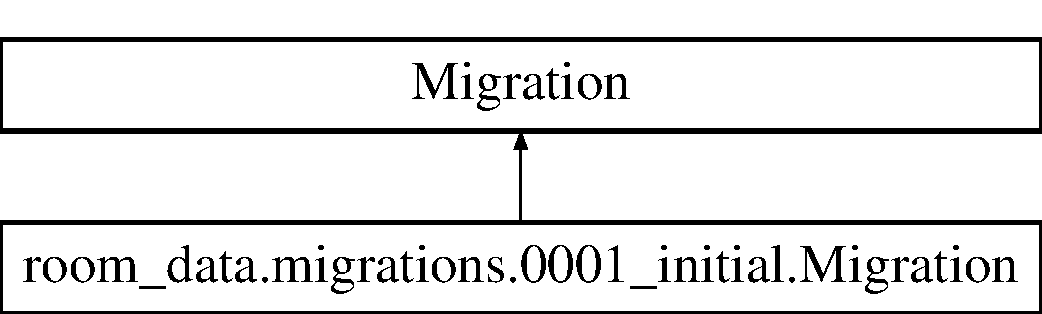
\includegraphics[height=2.000000cm]{classroom__data_1_1migrations_1_10001__initial_1_1_migration}
\end{center}
\end{figure}
\subsection*{Static Public Attributes}
\begin{DoxyCompactItemize}
\item 
\hypertarget{classroom__data_1_1migrations_1_10001__initial_1_1_migration_a381ac13c35311727d04e86e257323e0e}{{\bfseries initial} = True}\label{classroom__data_1_1migrations_1_10001__initial_1_1_migration_a381ac13c35311727d04e86e257323e0e}

\item 
list {\bfseries dependencies}
\item 
list {\bfseries operations}
\end{DoxyCompactItemize}


\subsection{Member Data Documentation}
\hypertarget{classroom__data_1_1migrations_1_10001__initial_1_1_migration_ad77b7bcddcbd5643b43e97daf5f789c3}{\index{room\-\_\-data\-::migrations\-::0001\-\_\-initial\-::\-Migration@{room\-\_\-data\-::migrations\-::0001\-\_\-initial\-::\-Migration}!dependencies@{dependencies}}
\index{dependencies@{dependencies}!room_data::migrations::0001_initial::Migration@{room\-\_\-data\-::migrations\-::0001\-\_\-initial\-::\-Migration}}
\subsubsection[{dependencies}]{\setlength{\rightskip}{0pt plus 5cm}list room\-\_\-data.\-migrations.\-0001\-\_\-initial.\-Migration.\-dependencies\hspace{0.3cm}{\ttfamily [static]}}}\label{classroom__data_1_1migrations_1_10001__initial_1_1_migration_ad77b7bcddcbd5643b43e97daf5f789c3}
{\bfseries Initial value\-:}
\begin{DoxyCode}
1 = [
2     ]
\end{DoxyCode}
\hypertarget{classroom__data_1_1migrations_1_10001__initial_1_1_migration_a30b36d46b2f4310cc0392eae634aa2bc}{\index{room\-\_\-data\-::migrations\-::0001\-\_\-initial\-::\-Migration@{room\-\_\-data\-::migrations\-::0001\-\_\-initial\-::\-Migration}!operations@{operations}}
\index{operations@{operations}!room_data::migrations::0001_initial::Migration@{room\-\_\-data\-::migrations\-::0001\-\_\-initial\-::\-Migration}}
\subsubsection[{operations}]{\setlength{\rightskip}{0pt plus 5cm}list room\-\_\-data.\-migrations.\-0001\-\_\-initial.\-Migration.\-operations\hspace{0.3cm}{\ttfamily [static]}}}\label{classroom__data_1_1migrations_1_10001__initial_1_1_migration_a30b36d46b2f4310cc0392eae634aa2bc}
{\bfseries Initial value\-:}
\begin{DoxyCode}
1 = [
2         migrations.CreateModel(
3             name=\textcolor{stringliteral}{'Room'},
4             fields=[
5                 (\textcolor{stringliteral}{'id'}, models.AutoField(auto\_created=\textcolor{keyword}{True}, primary\_key=\textcolor{keyword}{True}, serialize=\textcolor{keyword}{False}, verbose\_name=\textcolor{stringliteral}{
      'ID'})),
6                 (\textcolor{stringliteral}{'building'}, models.CharField(max\_length=20)),
7                 (\textcolor{stringliteral}{'room'}, models.IntegerField()),
8                 (\textcolor{stringliteral}{'capacity'}, models.IntegerField()),
9                 (\textcolor{stringliteral}{'type\_room'}, models.CharField(max\_length=100)),
10                 (\textcolor{stringliteral}{'division'}, models.CharField(max\_length=100)),
11                 (\textcolor{stringliteral}{'subject'}, models.CharField(max\_length=100)),
12                 (\textcolor{stringliteral}{'course\_style'}, models.CharField(max\_length=100)),
13             ],
14         ),
15     ]
\end{DoxyCode}


The documentation for this class was generated from the following file\-:\begin{DoxyCompactItemize}
\item 
/home/travis/build/\-Open-\/\-Source-\/\-Software-\/\-Development/class-\/scheduler/mysite/room\-\_\-data/migrations/0001\-\_\-initial.\-py\end{DoxyCompactItemize}

\hypertarget{classroom__data_1_1migrations_1_10002__auto__20180226__1350_1_1_migration}{\section{room\-\_\-data.\-migrations.0002\-\_\-auto\-\_\-20180226\-\_\-1350.Migration Class Reference}
\label{classroom__data_1_1migrations_1_10002__auto__20180226__1350_1_1_migration}\index{room\-\_\-data.\-migrations.\-0002\-\_\-auto\-\_\-20180226\-\_\-1350.\-Migration@{room\-\_\-data.\-migrations.\-0002\-\_\-auto\-\_\-20180226\-\_\-1350.\-Migration}}
}
Inheritance diagram for room\-\_\-data.\-migrations.0002\-\_\-auto\-\_\-20180226\-\_\-1350.Migration\-:\begin{figure}[H]
\begin{center}
\leavevmode
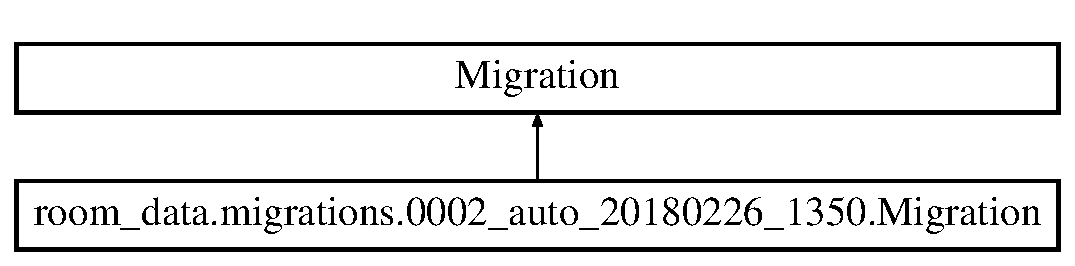
\includegraphics[height=2.000000cm]{classroom__data_1_1migrations_1_10002__auto__20180226__1350_1_1_migration}
\end{center}
\end{figure}
\subsection*{Static Public Attributes}
\begin{DoxyCompactItemize}
\item 
list {\bfseries dependencies}
\item 
list {\bfseries operations}
\end{DoxyCompactItemize}


\subsection{Member Data Documentation}
\hypertarget{classroom__data_1_1migrations_1_10002__auto__20180226__1350_1_1_migration_a31f1e9c6fcfef093a656c2c09c0958a1}{\index{room\-\_\-data\-::migrations\-::0002\-\_\-auto\-\_\-20180226\-\_\-1350\-::\-Migration@{room\-\_\-data\-::migrations\-::0002\-\_\-auto\-\_\-20180226\-\_\-1350\-::\-Migration}!dependencies@{dependencies}}
\index{dependencies@{dependencies}!room_data::migrations::0002_auto_20180226_1350::Migration@{room\-\_\-data\-::migrations\-::0002\-\_\-auto\-\_\-20180226\-\_\-1350\-::\-Migration}}
\subsubsection[{dependencies}]{\setlength{\rightskip}{0pt plus 5cm}list room\-\_\-data.\-migrations.\-0002\-\_\-auto\-\_\-20180226\-\_\-1350.\-Migration.\-dependencies\hspace{0.3cm}{\ttfamily [static]}}}\label{classroom__data_1_1migrations_1_10002__auto__20180226__1350_1_1_migration_a31f1e9c6fcfef093a656c2c09c0958a1}
{\bfseries Initial value\-:}
\begin{DoxyCode}
1 = [
2         (\textcolor{stringliteral}{'room\_data'}, \textcolor{stringliteral}{'0001\_initial'}),
3     ]
\end{DoxyCode}
\hypertarget{classroom__data_1_1migrations_1_10002__auto__20180226__1350_1_1_migration_affcbd4026c018e7d60fc5db2f6b460e3}{\index{room\-\_\-data\-::migrations\-::0002\-\_\-auto\-\_\-20180226\-\_\-1350\-::\-Migration@{room\-\_\-data\-::migrations\-::0002\-\_\-auto\-\_\-20180226\-\_\-1350\-::\-Migration}!operations@{operations}}
\index{operations@{operations}!room_data::migrations::0002_auto_20180226_1350::Migration@{room\-\_\-data\-::migrations\-::0002\-\_\-auto\-\_\-20180226\-\_\-1350\-::\-Migration}}
\subsubsection[{operations}]{\setlength{\rightskip}{0pt plus 5cm}list room\-\_\-data.\-migrations.\-0002\-\_\-auto\-\_\-20180226\-\_\-1350.\-Migration.\-operations\hspace{0.3cm}{\ttfamily [static]}}}\label{classroom__data_1_1migrations_1_10002__auto__20180226__1350_1_1_migration_affcbd4026c018e7d60fc5db2f6b460e3}
{\bfseries Initial value\-:}
\begin{DoxyCode}
1 = [
2         migrations.AlterField(
3             model\_name=\textcolor{stringliteral}{'room'},
4             name=\textcolor{stringliteral}{'capacity'},
5             field=models.CharField(max\_length=20),
6         ),
7         migrations.AlterField(
8             model\_name=\textcolor{stringliteral}{'room'},
9             name=\textcolor{stringliteral}{'room'},
10             field=models.CharField(max\_length=20),
11         ),
12     ]
\end{DoxyCode}


The documentation for this class was generated from the following file\-:\begin{DoxyCompactItemize}
\item 
/home/travis/build/\-Open-\/\-Source-\/\-Software-\/\-Development/class-\/scheduler/mysite/room\-\_\-data/migrations/0002\-\_\-auto\-\_\-20180226\-\_\-1350.\-py\end{DoxyCompactItemize}

\hypertarget{interfaceosd_1_1input_1_1_named}{\section{osd.\-input.\-Named Interface Reference}
\label{interfaceosd_1_1input_1_1_named}\index{osd.\-input.\-Named@{osd.\-input.\-Named}}
}
Inheritance diagram for osd.\-input.\-Named\-:\begin{figure}[H]
\begin{center}
\leavevmode
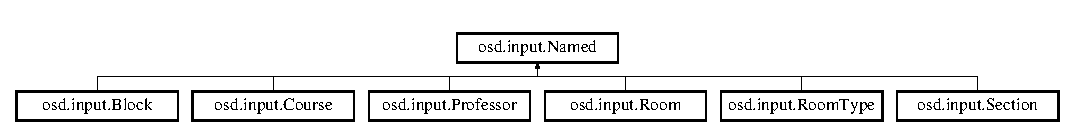
\includegraphics[height=1.393035cm]{interfaceosd_1_1input_1_1_named}
\end{center}
\end{figure}
\subsection*{Public Member Functions}
\begin{DoxyCompactItemize}
\item 
String \hyperlink{interfaceosd_1_1input_1_1_named_afde419887ef61b2a2c84328891f1a1ed}{get\-Name} ()
\end{DoxyCompactItemize}


\subsection{Detailed Description}
Represents osd.\-input types which have a name in their database table. 

\subsection{Member Function Documentation}
\hypertarget{interfaceosd_1_1input_1_1_named_afde419887ef61b2a2c84328891f1a1ed}{\index{osd\-::input\-::\-Named@{osd\-::input\-::\-Named}!get\-Name@{get\-Name}}
\index{get\-Name@{get\-Name}!osd::input::Named@{osd\-::input\-::\-Named}}
\subsubsection[{get\-Name}]{\setlength{\rightskip}{0pt plus 5cm}String osd.\-input.\-Named.\-get\-Name (
\begin{DoxyParamCaption}
{}
\end{DoxyParamCaption}
)}}\label{interfaceosd_1_1input_1_1_named_afde419887ef61b2a2c84328891f1a1ed}
\begin{DoxyReturn}{Returns}
The name of this object. 
\end{DoxyReturn}


Implemented in \hyperlink{interfaceosd_1_1input_1_1_professor_a2abdc30a0e45099e3d0dedf7ae303a58}{osd.\-input.\-Professor}.



The documentation for this interface was generated from the following file\-:\begin{DoxyCompactItemize}
\item 
/home/travis/build/\-Open-\/\-Source-\/\-Software-\/\-Development/class-\/scheduler/java/src/main/java/osd/input/Named.\-java\end{DoxyCompactItemize}

\hypertarget{classscheduler_1_1models_1_1_named}{\section{scheduler.\-models.\-Named Class Reference}
\label{classscheduler_1_1models_1_1_named}\index{scheduler.\-models.\-Named@{scheduler.\-models.\-Named}}
}
Inheritance diagram for scheduler.\-models.\-Named\-:\begin{figure}[H]
\begin{center}
\leavevmode
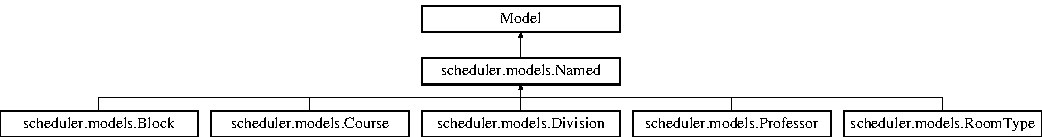
\includegraphics[height=1.846154cm]{classscheduler_1_1models_1_1_named}
\end{center}
\end{figure}
\subsection*{Classes}
\begin{DoxyCompactItemize}
\item 
class \hyperlink{classscheduler_1_1models_1_1_named_1_1_meta}{Meta}
\end{DoxyCompactItemize}
\subsection*{Public Member Functions}
\begin{DoxyCompactItemize}
\item 
\hypertarget{classscheduler_1_1models_1_1_named_a37b97c2fa4acbf5c61ca4cdff1410d47}{def {\bfseries \-\_\-\-\_\-str\-\_\-\-\_\-}}\label{classscheduler_1_1models_1_1_named_a37b97c2fa4acbf5c61ca4cdff1410d47}

\end{DoxyCompactItemize}
\subsection*{Static Public Attributes}
\begin{DoxyCompactItemize}
\item 
\hypertarget{classscheduler_1_1models_1_1_named_a5e5e18340ced82b633c6c913447d602f}{tuple {\bfseries name} = models.\-Char\-Field(max\-\_\-length=200, null=True)}\label{classscheduler_1_1models_1_1_named_a5e5e18340ced82b633c6c913447d602f}

\end{DoxyCompactItemize}


\subsection{Detailed Description}
\begin{DoxyVerb}    Gives better naming to things added manually
\end{DoxyVerb}
 

The documentation for this class was generated from the following file\-:\begin{DoxyCompactItemize}
\item 
/home/travis/build/\-Open-\/\-Source-\/\-Software-\/\-Development/class-\/scheduler/mysite/scheduler/models.\-py\end{DoxyCompactItemize}

\hypertarget{classosd_1_1util_1_1relation_1_1_one_to_many_relation_3_01_k_00_01_v_01_4}{\section{osd.\-util.\-relation.\-One\-To\-Many\-Relation$<$ K, V $>$ Class Reference}
\label{classosd_1_1util_1_1relation_1_1_one_to_many_relation_3_01_k_00_01_v_01_4}\index{osd.\-util.\-relation.\-One\-To\-Many\-Relation$<$ K, V $>$@{osd.\-util.\-relation.\-One\-To\-Many\-Relation$<$ K, V $>$}}
}
Inheritance diagram for osd.\-util.\-relation.\-One\-To\-Many\-Relation$<$ K, V $>$\-:\begin{figure}[H]
\begin{center}
\leavevmode
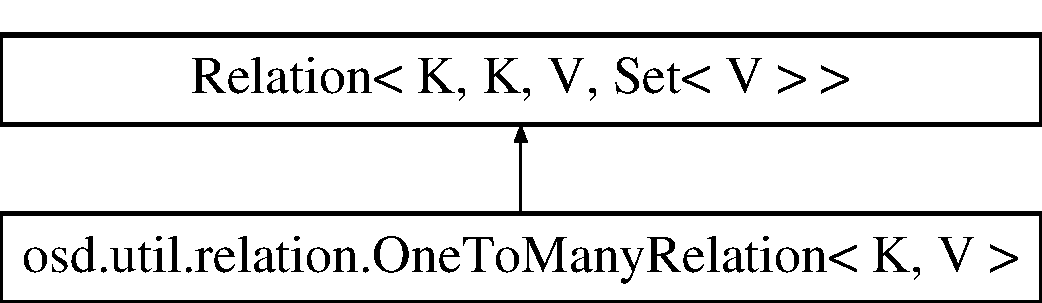
\includegraphics[height=2.000000cm]{classosd_1_1util_1_1relation_1_1_one_to_many_relation_3_01_k_00_01_v_01_4}
\end{center}
\end{figure}
\subsection*{Public Member Functions}
\begin{DoxyCompactItemize}
\item 
\hyperlink{classosd_1_1util_1_1relation_1_1_one_to_many_relation_3_01_k_00_01_v_01_4_ad85829fb137cb591ba07ff457918ecf2}{One\-To\-Many\-Relation} ()
\item 
\hyperlink{classosd_1_1util_1_1relation_1_1_one_to_many_relation_3_01_k_00_01_v_01_4_a9d73910df0fb6d24550316697fc4e47f}{One\-To\-Many\-Relation} (final Relation$<$ K, K, V, Set$<$ V $>$$>$ copy\-Of)
\item 
\hypertarget{classosd_1_1util_1_1relation_1_1_one_to_many_relation_3_01_k_00_01_v_01_4_a2cd287dedc12f05413334f50bcb4b9e1}{void {\bfseries add} (final K key, final V value)}\label{classosd_1_1util_1_1relation_1_1_one_to_many_relation_3_01_k_00_01_v_01_4_a2cd287dedc12f05413334f50bcb4b9e1}

\item 
\hypertarget{classosd_1_1util_1_1relation_1_1_one_to_many_relation_3_01_k_00_01_v_01_4_a23b9659f96a67b9a82acbe48d69dc0c5}{void {\bfseries remove} (final K key, final V value)}\label{classosd_1_1util_1_1relation_1_1_one_to_many_relation_3_01_k_00_01_v_01_4_a23b9659f96a67b9a82acbe48d69dc0c5}

\item 
\hypertarget{classosd_1_1util_1_1relation_1_1_one_to_many_relation_3_01_k_00_01_v_01_4_a3d817583e1123be6af8040d531eb13b5}{void {\bfseries remove} (final K key)}\label{classosd_1_1util_1_1relation_1_1_one_to_many_relation_3_01_k_00_01_v_01_4_a3d817583e1123be6af8040d531eb13b5}

\item 
\hypertarget{classosd_1_1util_1_1relation_1_1_one_to_many_relation_3_01_k_00_01_v_01_4_a3e74cebee1977d8f31e0760c074f6299}{Relation$<$ V, Set$<$ V $>$, K, K $>$ {\bfseries reversed} ()}\label{classosd_1_1util_1_1relation_1_1_one_to_many_relation_3_01_k_00_01_v_01_4_a3e74cebee1977d8f31e0760c074f6299}

\end{DoxyCompactItemize}
\subsection*{Protected Member Functions}
\begin{DoxyCompactItemize}
\item 
\hyperlink{classosd_1_1util_1_1relation_1_1_one_to_many_relation_3_01_k_00_01_v_01_4_a80cc67fa6eb42a2b27b9b65ddac3150f}{One\-To\-Many\-Relation} (final Map$<$ K, Set$<$ V $>$$>$ forward, final Map$<$ V, K $>$ reverse)
\end{DoxyCompactItemize}


\subsection{Constructor \& Destructor Documentation}
\hypertarget{classosd_1_1util_1_1relation_1_1_one_to_many_relation_3_01_k_00_01_v_01_4_ad85829fb137cb591ba07ff457918ecf2}{\index{osd\-::util\-::relation\-::\-One\-To\-Many\-Relation$<$ K, V $>$@{osd\-::util\-::relation\-::\-One\-To\-Many\-Relation$<$ K, V $>$}!One\-To\-Many\-Relation@{One\-To\-Many\-Relation}}
\index{One\-To\-Many\-Relation@{One\-To\-Many\-Relation}!osd::util::relation::OneToManyRelation< K, V >@{osd\-::util\-::relation\-::\-One\-To\-Many\-Relation$<$ K, V $>$}}
\subsubsection[{One\-To\-Many\-Relation}]{\setlength{\rightskip}{0pt plus 5cm}osd.\-util.\-relation.\-One\-To\-Many\-Relation$<$ K, V $>$.One\-To\-Many\-Relation (
\begin{DoxyParamCaption}
{}
\end{DoxyParamCaption}
)\hspace{0.3cm}{\ttfamily [inline]}}}\label{classosd_1_1util_1_1relation_1_1_one_to_many_relation_3_01_k_00_01_v_01_4_ad85829fb137cb591ba07ff457918ecf2}
Constructs a new relation with no data. \hypertarget{classosd_1_1util_1_1relation_1_1_one_to_many_relation_3_01_k_00_01_v_01_4_a9d73910df0fb6d24550316697fc4e47f}{\index{osd\-::util\-::relation\-::\-One\-To\-Many\-Relation$<$ K, V $>$@{osd\-::util\-::relation\-::\-One\-To\-Many\-Relation$<$ K, V $>$}!One\-To\-Many\-Relation@{One\-To\-Many\-Relation}}
\index{One\-To\-Many\-Relation@{One\-To\-Many\-Relation}!osd::util::relation::OneToManyRelation< K, V >@{osd\-::util\-::relation\-::\-One\-To\-Many\-Relation$<$ K, V $>$}}
\subsubsection[{One\-To\-Many\-Relation}]{\setlength{\rightskip}{0pt plus 5cm}osd.\-util.\-relation.\-One\-To\-Many\-Relation$<$ K, V $>$.One\-To\-Many\-Relation (
\begin{DoxyParamCaption}
\item[{final Relation$<$ K, K, V, Set$<$ V $>$$>$}]{copy\-Of}
\end{DoxyParamCaption}
)\hspace{0.3cm}{\ttfamily [inline]}}}\label{classosd_1_1util_1_1relation_1_1_one_to_many_relation_3_01_k_00_01_v_01_4_a9d73910df0fb6d24550316697fc4e47f}
Copy constructor. The original relation and the copy are completely separate; changes to one will not be reflected in the other. 
\begin{DoxyParams}{Parameters}
{\em copy\-Of} & the relation to copy \\
\hline
\end{DoxyParams}
\hypertarget{classosd_1_1util_1_1relation_1_1_one_to_many_relation_3_01_k_00_01_v_01_4_a80cc67fa6eb42a2b27b9b65ddac3150f}{\index{osd\-::util\-::relation\-::\-One\-To\-Many\-Relation$<$ K, V $>$@{osd\-::util\-::relation\-::\-One\-To\-Many\-Relation$<$ K, V $>$}!One\-To\-Many\-Relation@{One\-To\-Many\-Relation}}
\index{One\-To\-Many\-Relation@{One\-To\-Many\-Relation}!osd::util::relation::OneToManyRelation< K, V >@{osd\-::util\-::relation\-::\-One\-To\-Many\-Relation$<$ K, V $>$}}
\subsubsection[{One\-To\-Many\-Relation}]{\setlength{\rightskip}{0pt plus 5cm}osd.\-util.\-relation.\-One\-To\-Many\-Relation$<$ K, V $>$.One\-To\-Many\-Relation (
\begin{DoxyParamCaption}
\item[{final Map$<$ K, Set$<$ V $>$$>$}]{forward, }
\item[{final Map$<$ V, K $>$}]{reverse}
\end{DoxyParamCaption}
)\hspace{0.3cm}{\ttfamily [inline]}, {\ttfamily [protected]}}}\label{classosd_1_1util_1_1relation_1_1_one_to_many_relation_3_01_k_00_01_v_01_4_a80cc67fa6eb42a2b27b9b65ddac3150f}
View constructor. The relation's maps are supplied directly, and it will read and write to them as appropriate. Be careful with this. 
\begin{DoxyParams}{Parameters}
{\em forward} & the forward map \\
\hline
{\em reverse} & the reverse map \\
\hline
\end{DoxyParams}


The documentation for this class was generated from the following file\-:\begin{DoxyCompactItemize}
\item 
/home/travis/build/\-Open-\/\-Source-\/\-Software-\/\-Development/class-\/scheduler/java/src/main/java/osd/util/relation/One\-To\-Many\-Relation.\-java\end{DoxyCompactItemize}

\hypertarget{classscheduler_1_1csv__parser_1_1_parse_mode}{\section{scheduler.\-csv\-\_\-parser.\-Parse\-Mode Class Reference}
\label{classscheduler_1_1csv__parser_1_1_parse_mode}\index{scheduler.\-csv\-\_\-parser.\-Parse\-Mode@{scheduler.\-csv\-\_\-parser.\-Parse\-Mode}}
}
Inheritance diagram for scheduler.\-csv\-\_\-parser.\-Parse\-Mode\-:\begin{figure}[H]
\begin{center}
\leavevmode
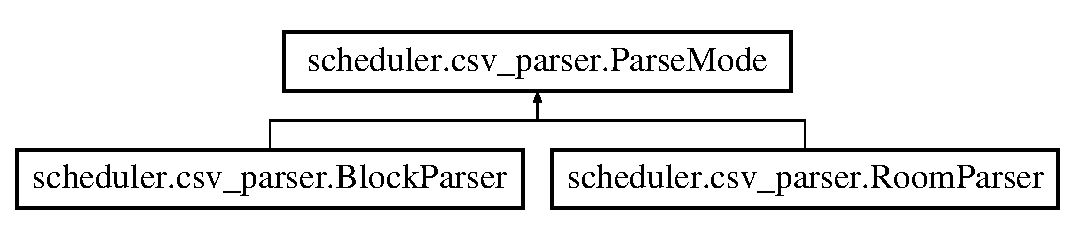
\includegraphics[height=2.000000cm]{classscheduler_1_1csv__parser_1_1_parse_mode}
\end{center}
\end{figure}
\subsection*{Public Member Functions}
\begin{DoxyCompactItemize}
\item 
def \hyperlink{classscheduler_1_1csv__parser_1_1_parse_mode_a3bc8ae2168d14c9f956528bf32023a3a}{register}
\item 
\hypertarget{classscheduler_1_1csv__parser_1_1_parse_mode_ad8e4121ce73986f2a07f939c666a2ad4}{def {\bfseries \-\_\-\-\_\-init\-\_\-\-\_\-}}\label{classscheduler_1_1csv__parser_1_1_parse_mode_ad8e4121ce73986f2a07f939c666a2ad4}

\item 
def \hyperlink{classscheduler_1_1csv__parser_1_1_parse_mode_a0feea2cd6393529d3606b348565bb58d}{can\-\_\-parse}
\item 
def \hyperlink{classscheduler_1_1csv__parser_1_1_parse_mode_a85b23beeadbaf1d1ed4046948928db9a}{for\-\_\-header}
\item 
def \hyperlink{classscheduler_1_1csv__parser_1_1_parse_mode_ab0e0daafe895143ae2c0042b1d77b1bb}{add\-\_\-row}
\item 
def \hyperlink{classscheduler_1_1csv__parser_1_1_parse_mode_af96a04e247153f76b58d7963b1721c4c}{get\-\_\-models}
\item 
def \hyperlink{classscheduler_1_1csv__parser_1_1_parse_mode_a4ee02dc3d582a3b222fe84db69731c91}{add\-\_\-row\-\_\-impl}
\end{DoxyCompactItemize}
\subsection*{Public Attributes}
\begin{DoxyCompactItemize}
\item 
\hypertarget{classscheduler_1_1csv__parser_1_1_parse_mode_a13cc81cc8f8e63d9aca98934beda8c67}{{\bfseries header}}\label{classscheduler_1_1csv__parser_1_1_parse_mode_a13cc81cc8f8e63d9aca98934beda8c67}

\end{DoxyCompactItemize}
\subsection*{Static Public Attributes}
\begin{DoxyCompactItemize}
\item 
\hypertarget{classscheduler_1_1csv__parser_1_1_parse_mode_a649baaf5bb93b19ddf00ace72debf871}{list {\bfseries modes} = \mbox{[}$\,$\mbox{]}}\label{classscheduler_1_1csv__parser_1_1_parse_mode_a649baaf5bb93b19ddf00ace72debf871}

\end{DoxyCompactItemize}


\subsection{Detailed Description}
\begin{DoxyVerb}A CSV schema. Schemas should be created by extending this class
and decorating them with @ParseMode.register. Such subclasses MUST
declare the columns they care about with a static tuple named
'columns'.

Args:
    header (list str): The CSV's header.
\end{DoxyVerb}
 

\subsection{Member Function Documentation}
\hypertarget{classscheduler_1_1csv__parser_1_1_parse_mode_ab0e0daafe895143ae2c0042b1d77b1bb}{\index{scheduler\-::csv\-\_\-parser\-::\-Parse\-Mode@{scheduler\-::csv\-\_\-parser\-::\-Parse\-Mode}!add\-\_\-row@{add\-\_\-row}}
\index{add\-\_\-row@{add\-\_\-row}!scheduler::csv_parser::ParseMode@{scheduler\-::csv\-\_\-parser\-::\-Parse\-Mode}}
\subsubsection[{add\-\_\-row}]{\setlength{\rightskip}{0pt plus 5cm}def scheduler.\-csv\-\_\-parser.\-Parse\-Mode.\-add\-\_\-row (
\begin{DoxyParamCaption}
\item[{}]{self, }
\item[{}]{row}
\end{DoxyParamCaption}
)}}\label{classscheduler_1_1csv__parser_1_1_parse_mode_ab0e0daafe895143ae2c0042b1d77b1bb}
\begin{DoxyVerb}Parse a single CSV row and store it.\end{DoxyVerb}
 \hypertarget{classscheduler_1_1csv__parser_1_1_parse_mode_a4ee02dc3d582a3b222fe84db69731c91}{\index{scheduler\-::csv\-\_\-parser\-::\-Parse\-Mode@{scheduler\-::csv\-\_\-parser\-::\-Parse\-Mode}!add\-\_\-row\-\_\-impl@{add\-\_\-row\-\_\-impl}}
\index{add\-\_\-row\-\_\-impl@{add\-\_\-row\-\_\-impl}!scheduler::csv_parser::ParseMode@{scheduler\-::csv\-\_\-parser\-::\-Parse\-Mode}}
\subsubsection[{add\-\_\-row\-\_\-impl}]{\setlength{\rightskip}{0pt plus 5cm}def scheduler.\-csv\-\_\-parser.\-Parse\-Mode.\-add\-\_\-row\-\_\-impl (
\begin{DoxyParamCaption}
\item[{}]{self, }
\item[{}]{row}
\end{DoxyParamCaption}
)}}\label{classscheduler_1_1csv__parser_1_1_parse_mode_a4ee02dc3d582a3b222fe84db69731c91}
\begin{DoxyVerb}Hook to define parse logic.\end{DoxyVerb}
 \hypertarget{classscheduler_1_1csv__parser_1_1_parse_mode_a0feea2cd6393529d3606b348565bb58d}{\index{scheduler\-::csv\-\_\-parser\-::\-Parse\-Mode@{scheduler\-::csv\-\_\-parser\-::\-Parse\-Mode}!can\-\_\-parse@{can\-\_\-parse}}
\index{can\-\_\-parse@{can\-\_\-parse}!scheduler::csv_parser::ParseMode@{scheduler\-::csv\-\_\-parser\-::\-Parse\-Mode}}
\subsubsection[{can\-\_\-parse}]{\setlength{\rightskip}{0pt plus 5cm}def scheduler.\-csv\-\_\-parser.\-Parse\-Mode.\-can\-\_\-parse (
\begin{DoxyParamCaption}
\item[{}]{cls, }
\item[{}]{header}
\end{DoxyParamCaption}
)}}\label{classscheduler_1_1csv__parser_1_1_parse_mode_a0feea2cd6393529d3606b348565bb58d}
\begin{DoxyVerb}Checks if all this mode's columns are in the header.\end{DoxyVerb}
 \hypertarget{classscheduler_1_1csv__parser_1_1_parse_mode_a85b23beeadbaf1d1ed4046948928db9a}{\index{scheduler\-::csv\-\_\-parser\-::\-Parse\-Mode@{scheduler\-::csv\-\_\-parser\-::\-Parse\-Mode}!for\-\_\-header@{for\-\_\-header}}
\index{for\-\_\-header@{for\-\_\-header}!scheduler::csv_parser::ParseMode@{scheduler\-::csv\-\_\-parser\-::\-Parse\-Mode}}
\subsubsection[{for\-\_\-header}]{\setlength{\rightskip}{0pt plus 5cm}def scheduler.\-csv\-\_\-parser.\-Parse\-Mode.\-for\-\_\-header (
\begin{DoxyParamCaption}
\item[{}]{cls, }
\item[{}]{header}
\end{DoxyParamCaption}
)}}\label{classscheduler_1_1csv__parser_1_1_parse_mode_a85b23beeadbaf1d1ed4046948928db9a}
\begin{DoxyVerb}Gets a parse mode for a header or fails with an IndexError.\end{DoxyVerb}
 \hypertarget{classscheduler_1_1csv__parser_1_1_parse_mode_af96a04e247153f76b58d7963b1721c4c}{\index{scheduler\-::csv\-\_\-parser\-::\-Parse\-Mode@{scheduler\-::csv\-\_\-parser\-::\-Parse\-Mode}!get\-\_\-models@{get\-\_\-models}}
\index{get\-\_\-models@{get\-\_\-models}!scheduler::csv_parser::ParseMode@{scheduler\-::csv\-\_\-parser\-::\-Parse\-Mode}}
\subsubsection[{get\-\_\-models}]{\setlength{\rightskip}{0pt plus 5cm}def scheduler.\-csv\-\_\-parser.\-Parse\-Mode.\-get\-\_\-models (
\begin{DoxyParamCaption}
\item[{}]{self}
\end{DoxyParamCaption}
)}}\label{classscheduler_1_1csv__parser_1_1_parse_mode_af96a04e247153f76b58d7963b1721c4c}
\begin{DoxyVerb}Gets the models corresponding to our CSV rows.\end{DoxyVerb}
 \hypertarget{classscheduler_1_1csv__parser_1_1_parse_mode_a3bc8ae2168d14c9f956528bf32023a3a}{\index{scheduler\-::csv\-\_\-parser\-::\-Parse\-Mode@{scheduler\-::csv\-\_\-parser\-::\-Parse\-Mode}!register@{register}}
\index{register@{register}!scheduler::csv_parser::ParseMode@{scheduler\-::csv\-\_\-parser\-::\-Parse\-Mode}}
\subsubsection[{register}]{\setlength{\rightskip}{0pt plus 5cm}def scheduler.\-csv\-\_\-parser.\-Parse\-Mode.\-register (
\begin{DoxyParamCaption}
\item[{}]{cls, }
\item[{}]{mode}
\end{DoxyParamCaption}
)}}\label{classscheduler_1_1csv__parser_1_1_parse_mode_a3bc8ae2168d14c9f956528bf32023a3a}
\begin{DoxyVerb}Automatically registers this parse mode.\end{DoxyVerb}
 

The documentation for this class was generated from the following file\-:\begin{DoxyCompactItemize}
\item 
/home/travis/build/\-Open-\/\-Source-\/\-Software-\/\-Development/class-\/scheduler/mysite/scheduler/csv\-\_\-parser.\-py\end{DoxyCompactItemize}

\hypertarget{classosd_1_1input_1_1placeholder_1_1_placeholder_module}{\section{osd.\-input.\-placeholder.\-Placeholder\-Module Class Reference}
\label{classosd_1_1input_1_1placeholder_1_1_placeholder_module}\index{osd.\-input.\-placeholder.\-Placeholder\-Module@{osd.\-input.\-placeholder.\-Placeholder\-Module}}
}


The documentation for this class was generated from the following file\-:\begin{DoxyCompactItemize}
\item 
/home/travis/build/\-Open-\/\-Source-\/\-Software-\/\-Development/class-\/scheduler/java/src/main/java/osd/input/placeholder/Placeholder\-Module.\-java\end{DoxyCompactItemize}

\hypertarget{classpolls_1_1apps_1_1_polls_config}{\section{polls.\-apps.\-Polls\-Config Class Reference}
\label{classpolls_1_1apps_1_1_polls_config}\index{polls.\-apps.\-Polls\-Config@{polls.\-apps.\-Polls\-Config}}
}
Inheritance diagram for polls.\-apps.\-Polls\-Config\-:\begin{figure}[H]
\begin{center}
\leavevmode
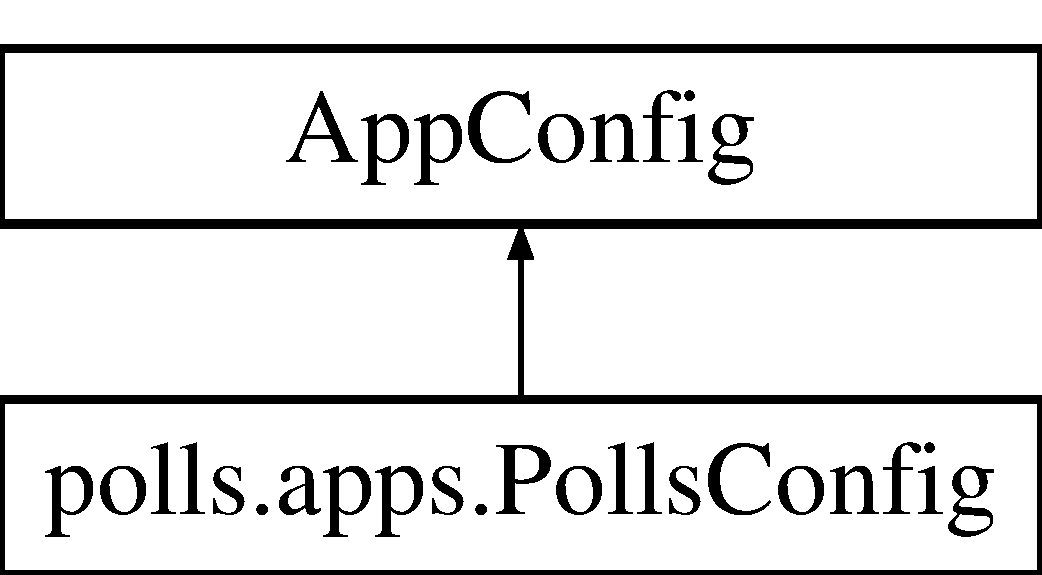
\includegraphics[height=2.000000cm]{classpolls_1_1apps_1_1_polls_config}
\end{center}
\end{figure}
\subsection*{Static Public Attributes}
\begin{DoxyCompactItemize}
\item 
\hypertarget{classpolls_1_1apps_1_1_polls_config_a969f90ecc73447a69938dc41cf33e29e}{string {\bfseries name} = 'polls'}\label{classpolls_1_1apps_1_1_polls_config_a969f90ecc73447a69938dc41cf33e29e}

\end{DoxyCompactItemize}


The documentation for this class was generated from the following file\-:\begin{DoxyCompactItemize}
\item 
/home/travis/build/\-Open-\/\-Source-\/\-Software-\/\-Development/class-\/scheduler/mysite/polls/apps.\-py\end{DoxyCompactItemize}

\hypertarget{interfaceosd_1_1considerations_1_1_preference}{\section{osd.\-considerations.\-Preference Interface Reference}
\label{interfaceosd_1_1considerations_1_1_preference}\index{osd.\-considerations.\-Preference@{osd.\-considerations.\-Preference}}
}
Inheritance diagram for osd.\-considerations.\-Preference\-:\begin{figure}[H]
\begin{center}
\leavevmode
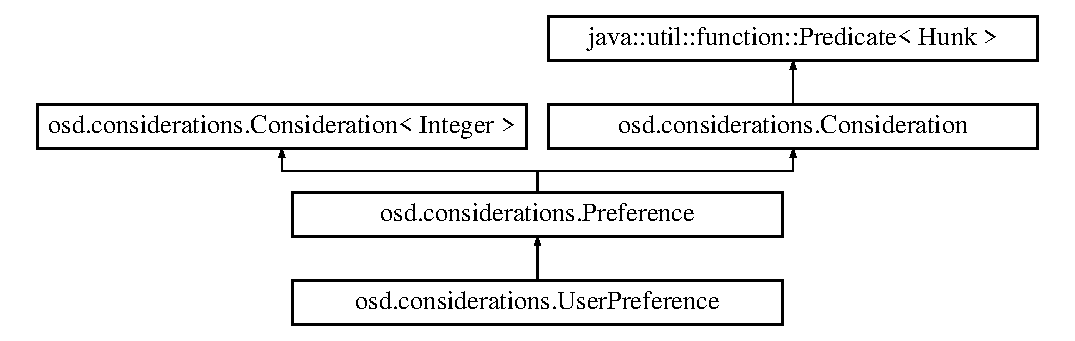
\includegraphics[height=4.000000cm]{interfaceosd_1_1considerations_1_1_preference}
\end{center}
\end{figure}
\subsection*{Public Member Functions}
\begin{DoxyCompactItemize}
\item 
\hypertarget{interfaceosd_1_1considerations_1_1_preference_ad9af6831a7b789685a22037c7abdf008}{default int {\bfseries evaluate} (final \hyperlink{classosd_1_1output_1_1_hunk}{Hunk} hunk)}\label{interfaceosd_1_1considerations_1_1_preference_ad9af6831a7b789685a22037c7abdf008}

\item 
\hypertarget{interfaceosd_1_1considerations_1_1_preference_ad814027d6d3a6e773fa067299bc21456}{int {\bfseries worth} ()}\label{interfaceosd_1_1considerations_1_1_preference_ad814027d6d3a6e773fa067299bc21456}

\end{DoxyCompactItemize}


The documentation for this interface was generated from the following file\-:\begin{DoxyCompactItemize}
\item 
/home/travis/build/\-Open-\/\-Source-\/\-Software-\/\-Development/class-\/scheduler/java/src/main/java/osd/considerations/Preference.\-java\end{DoxyCompactItemize}

\hypertarget{classscheduler_1_1models_1_1_pregen_section}{\section{scheduler.\-models.\-Pregen\-Section Class Reference}
\label{classscheduler_1_1models_1_1_pregen_section}\index{scheduler.\-models.\-Pregen\-Section@{scheduler.\-models.\-Pregen\-Section}}
}
Inheritance diagram for scheduler.\-models.\-Pregen\-Section\-:\begin{figure}[H]
\begin{center}
\leavevmode
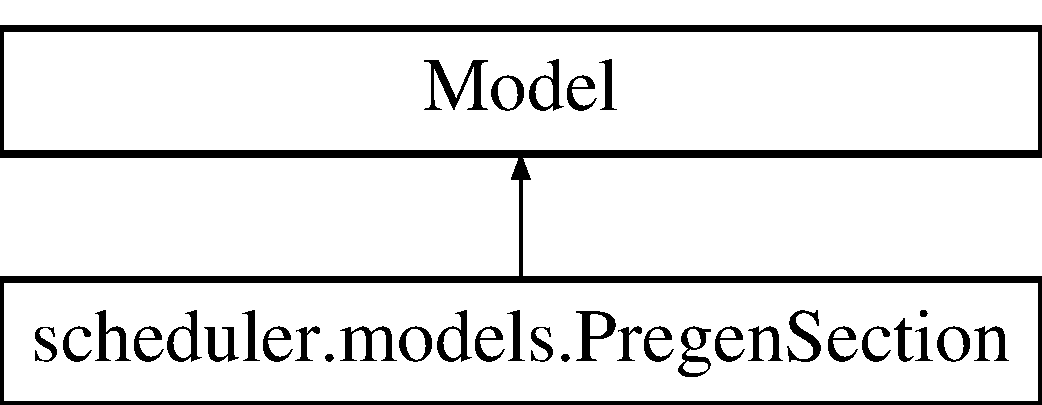
\includegraphics[height=2.000000cm]{classscheduler_1_1models_1_1_pregen_section}
\end{center}
\end{figure}
\subsection*{Public Member Functions}
\begin{DoxyCompactItemize}
\item 
\hypertarget{classscheduler_1_1models_1_1_pregen_section_a0f46c875c91c38646fdefea75fb5d652}{def {\bfseries \-\_\-\-\_\-str\-\_\-\-\_\-}}\label{classscheduler_1_1models_1_1_pregen_section_a0f46c875c91c38646fdefea75fb5d652}

\end{DoxyCompactItemize}
\subsection*{Static Public Attributes}
\begin{DoxyCompactItemize}
\item 
\hypertarget{classscheduler_1_1models_1_1_pregen_section_a3eafd0071b89cf3573c5f47c9194f848}{tuple {\bfseries course} = models.\-Foreign\-Key(\hyperlink{classscheduler_1_1models_1_1_course}{Course}, on\-\_\-delete=models.\-C\-A\-S\-C\-A\-D\-E)}\label{classscheduler_1_1models_1_1_pregen_section_a3eafd0071b89cf3573c5f47c9194f848}

\item 
\hypertarget{classscheduler_1_1models_1_1_pregen_section_ae51c6af4b08756b861dc5fe9bec2e203}{tuple {\bfseries suffix} = models.\-Char\-Field(max\-\_\-length=50)}\label{classscheduler_1_1models_1_1_pregen_section_ae51c6af4b08756b861dc5fe9bec2e203}

\end{DoxyCompactItemize}


\subsection{Detailed Description}
\begin{DoxyVerb}    TODO: Finish Table
    TODO: Documentation
\end{DoxyVerb}
 

The documentation for this class was generated from the following file\-:\begin{DoxyCompactItemize}
\item 
/home/travis/build/\-Open-\/\-Source-\/\-Software-\/\-Development/class-\/scheduler/mysite/scheduler/models.\-py\end{DoxyCompactItemize}

\hypertarget{interfaceosd_1_1input_1_1_professor}{\section{osd.\-input.\-Professor Class Reference}
\label{interfaceosd_1_1input_1_1_professor}\index{osd.\-input.\-Professor@{osd.\-input.\-Professor}}
}
Inheritance diagram for osd.\-input.\-Professor\-:\begin{figure}[H]
\begin{center}
\leavevmode
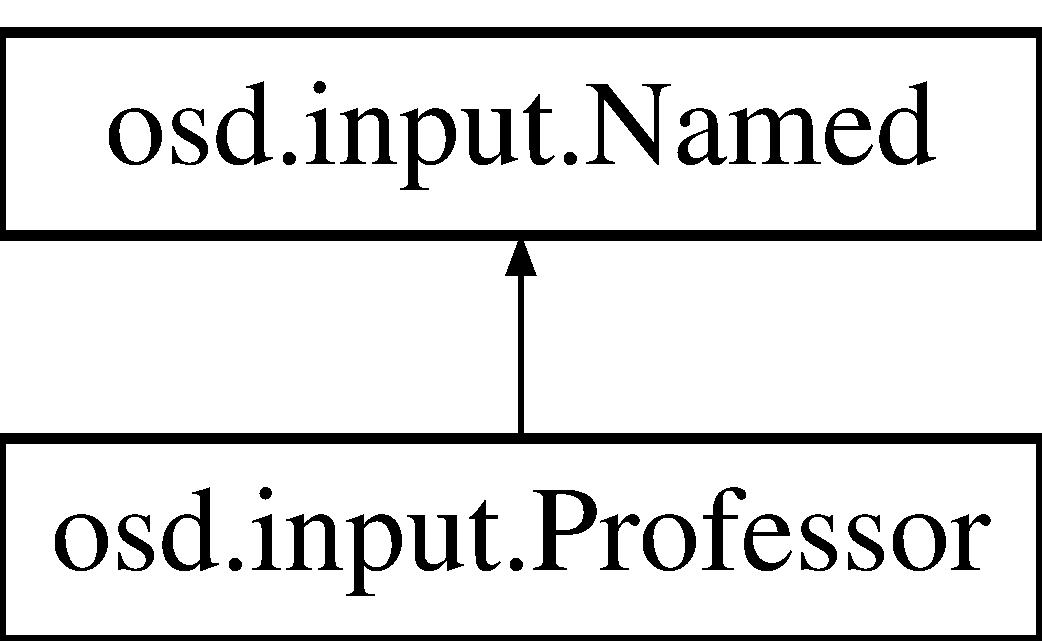
\includegraphics[height=2.000000cm]{interfaceosd_1_1input_1_1_professor}
\end{center}
\end{figure}
\subsection*{Public Member Functions}
\begin{DoxyCompactItemize}
\item 
default int \hyperlink{interfaceosd_1_1input_1_1_professor_a61a4ffd17d3360fbcc52c021aaf3f752}{get\-Course\-Capacity} ()
\item 
\hypertarget{interfaceosd_1_1input_1_1_professor_aa4ae8d22fffce4414523a44a7b240892}{{\bfseries Professor} (int t\-Id, String t\-Name, \hyperlink{interfaceosd_1_1input_1_1_course}{Course}\mbox{[}$\,$\mbox{]} t\-Courses, boolean t\-Is\-Adjunct)}\label{interfaceosd_1_1input_1_1_professor_aa4ae8d22fffce4414523a44a7b240892}

\item 
\hypertarget{interfaceosd_1_1input_1_1_professor_af095dc27a8f6709cd9eb3379d29db8f4}{int {\bfseries get\-Id} ()}\label{interfaceosd_1_1input_1_1_professor_af095dc27a8f6709cd9eb3379d29db8f4}

\item 
String \hyperlink{interfaceosd_1_1input_1_1_professor_a2abdc30a0e45099e3d0dedf7ae303a58}{get\-Name} ()
\item 
\hypertarget{interfaceosd_1_1input_1_1_professor_a97280839a452c7b0697547e7854b4458}{\hyperlink{interfaceosd_1_1input_1_1_course}{Course}\mbox{[}$\,$\mbox{]} {\bfseries get\-Courses} ()}\label{interfaceosd_1_1input_1_1_professor_a97280839a452c7b0697547e7854b4458}

\item 
\hypertarget{interfaceosd_1_1input_1_1_professor_a40ad65f1dc4528a9d67621367156458b}{int {\bfseries get\-Scheduled\-Sections} ()}\label{interfaceosd_1_1input_1_1_professor_a40ad65f1dc4528a9d67621367156458b}

\item 
\hypertarget{interfaceosd_1_1input_1_1_professor_adfc653b2b31e44689db9e5c7b194ebbb}{boolean {\bfseries is\-Adjunct} ()}\label{interfaceosd_1_1input_1_1_professor_adfc653b2b31e44689db9e5c7b194ebbb}

\end{DoxyCompactItemize}


\subsection{Detailed Description}
Represents a professor. The most important characteristic of a professor that isn't covered by the preferences system is their course capacity. 

\subsection{Member Function Documentation}
\hypertarget{interfaceosd_1_1input_1_1_professor_a61a4ffd17d3360fbcc52c021aaf3f752}{\index{osd\-::input\-::\-Professor@{osd\-::input\-::\-Professor}!get\-Course\-Capacity@{get\-Course\-Capacity}}
\index{get\-Course\-Capacity@{get\-Course\-Capacity}!osd::input::Professor@{osd\-::input\-::\-Professor}}
\subsubsection[{get\-Course\-Capacity}]{\setlength{\rightskip}{0pt plus 5cm}default int osd.\-input.\-Professor.\-get\-Course\-Capacity (
\begin{DoxyParamCaption}
{}
\end{DoxyParamCaption}
)\hspace{0.3cm}{\ttfamily [inline]}}}\label{interfaceosd_1_1input_1_1_professor_a61a4ffd17d3360fbcc52c021aaf3f752}
Gets the maximum number of course sections this professor can teach. Defaults to 4. \begin{DoxyReturn}{Returns}
the maximum number of course sections this professor can teach 
\end{DoxyReturn}
\hypertarget{interfaceosd_1_1input_1_1_professor_a2abdc30a0e45099e3d0dedf7ae303a58}{\index{osd\-::input\-::\-Professor@{osd\-::input\-::\-Professor}!get\-Name@{get\-Name}}
\index{get\-Name@{get\-Name}!osd::input::Professor@{osd\-::input\-::\-Professor}}
\subsubsection[{get\-Name}]{\setlength{\rightskip}{0pt plus 5cm}String osd.\-input.\-Professor.\-get\-Name (
\begin{DoxyParamCaption}
{}
\end{DoxyParamCaption}
)\hspace{0.3cm}{\ttfamily [inline]}}}\label{interfaceosd_1_1input_1_1_professor_a2abdc30a0e45099e3d0dedf7ae303a58}
\begin{DoxyReturn}{Returns}
The name of this object. 
\end{DoxyReturn}


Implements \hyperlink{interfaceosd_1_1input_1_1_named_afde419887ef61b2a2c84328891f1a1ed}{osd.\-input.\-Named}.



The documentation for this class was generated from the following file\-:\begin{DoxyCompactItemize}
\item 
/home/travis/build/\-Open-\/\-Source-\/\-Software-\/\-Development/class-\/scheduler/java/src/main/java/osd/input/Professor.\-java\end{DoxyCompactItemize}

\hypertarget{classscheduler_1_1models_1_1_professor}{\section{scheduler.\-models.\-Professor Class Reference}
\label{classscheduler_1_1models_1_1_professor}\index{scheduler.\-models.\-Professor@{scheduler.\-models.\-Professor}}
}
Inheritance diagram for scheduler.\-models.\-Professor\-:\begin{figure}[H]
\begin{center}
\leavevmode
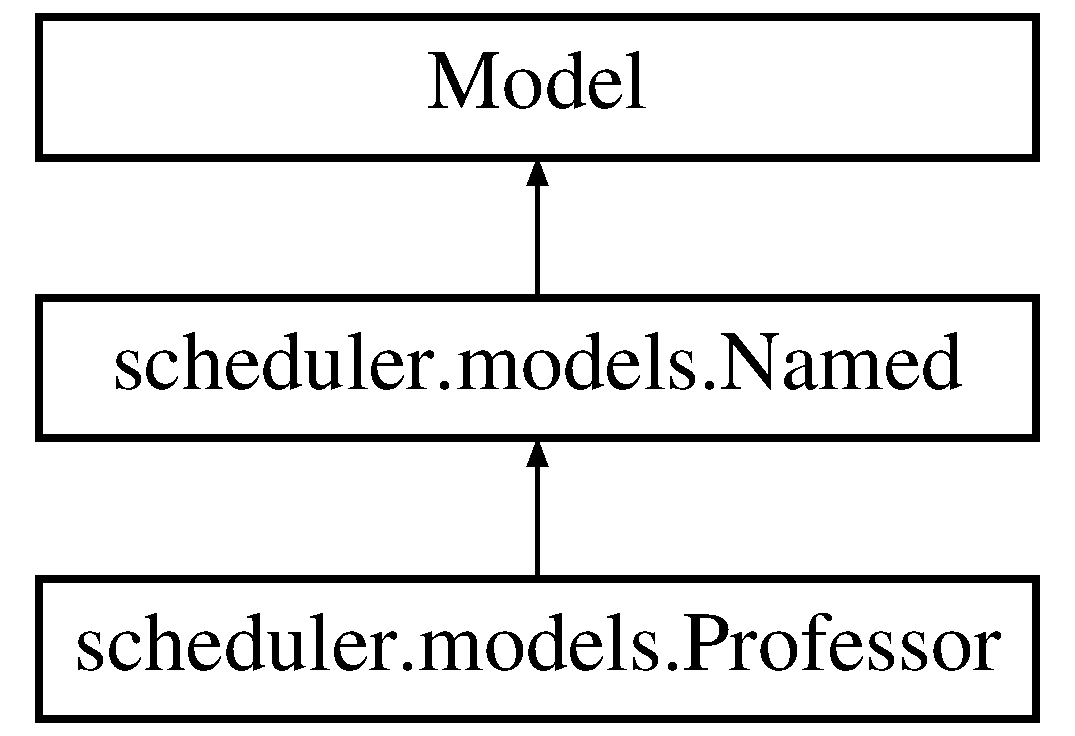
\includegraphics[height=3.000000cm]{classscheduler_1_1models_1_1_professor}
\end{center}
\end{figure}
\subsection*{Static Public Attributes}
\begin{DoxyCompactItemize}
\item 
\hypertarget{classscheduler_1_1models_1_1_professor_adf91e6bff4702170c31cb6135f23f31b}{tuple {\bfseries division} = models.\-Foreign\-Key(\hyperlink{classscheduler_1_1models_1_1_division}{Division}, on\-\_\-delete=models.\-C\-A\-S\-C\-A\-D\-E)}\label{classscheduler_1_1models_1_1_professor_adf91e6bff4702170c31cb6135f23f31b}

\item 
\hypertarget{classscheduler_1_1models_1_1_professor_a5a76821dd158b7ee380cac02a95ef14f}{tuple {\bfseries first} = models.\-Char\-Field(max\-\_\-length=20, null=True, blank=True)}\label{classscheduler_1_1models_1_1_professor_a5a76821dd158b7ee380cac02a95ef14f}

\item 
\hypertarget{classscheduler_1_1models_1_1_professor_a399cc5731fa62ed365a91c4c1dfe45d0}{tuple {\bfseries last} = models.\-Char\-Field(max\-\_\-length=20, null=True, blank=True)}\label{classscheduler_1_1models_1_1_professor_a399cc5731fa62ed365a91c4c1dfe45d0}

\item 
\hypertarget{classscheduler_1_1models_1_1_professor_a49cca96860ed2452e86fc3877ad9d767}{tuple {\bfseries qualifications} = models.\-Many\-To\-Many\-Field(\hyperlink{classscheduler_1_1models_1_1_course}{Course})}\label{classscheduler_1_1models_1_1_professor_a49cca96860ed2452e86fc3877ad9d767}

\end{DoxyCompactItemize}
\subsection*{Additional Inherited Members}


\subsection{Detailed Description}
\begin{DoxyVerb}    Table: Professor
    PrimaryKey: Autogenerated ID
    Columns:
        division: ForeignKey Division
        first: CharField(max_length=20)
            - Professors First Name (ex: James)
        last: CharField(max_length=20)
            -Professor Last Name (ex: Wilson)
        qualifications: ManyToManyField with Course
            -Each professor teaches multiple courses 
\end{DoxyVerb}
 

The documentation for this class was generated from the following file\-:\begin{DoxyCompactItemize}
\item 
/home/travis/build/\-Open-\/\-Source-\/\-Software-\/\-Development/class-\/scheduler/mysite/scheduler/models.\-py\end{DoxyCompactItemize}

\hypertarget{classosd_1_1input_1_1_professor_factory}{\section{osd.\-input.\-Professor\-Factory Class Reference}
\label{classosd_1_1input_1_1_professor_factory}\index{osd.\-input.\-Professor\-Factory@{osd.\-input.\-Professor\-Factory}}
}
Inheritance diagram for osd.\-input.\-Professor\-Factory\-:\begin{figure}[H]
\begin{center}
\leavevmode
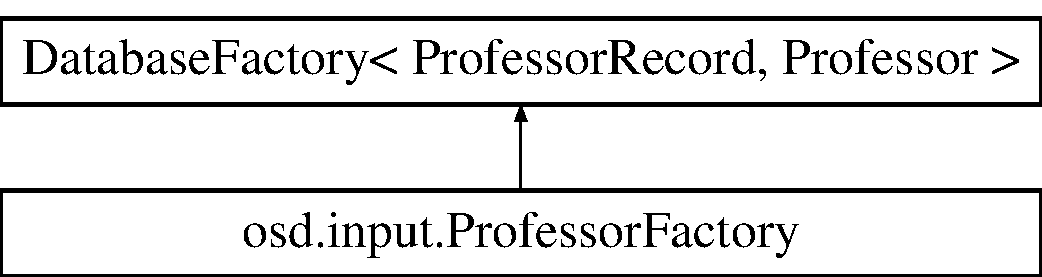
\includegraphics[height=2.000000cm]{classosd_1_1input_1_1_professor_factory}
\end{center}
\end{figure}
\subsection*{Public Member Functions}
\begin{DoxyCompactItemize}
\item 
\hypertarget{classosd_1_1input_1_1_professor_factory_a2ac185fdaf67e1ca4eeb86cd4209c277}{\hyperlink{interfaceosd_1_1input_1_1_professor}{Professor} {\bfseries create} (final \hyperlink{classosd_1_1database_1_1_professor_record}{Professor\-Record} record)}\label{classosd_1_1input_1_1_professor_factory_a2ac185fdaf67e1ca4eeb86cd4209c277}

\end{DoxyCompactItemize}


The documentation for this class was generated from the following file\-:\begin{DoxyCompactItemize}
\item 
/home/travis/build/\-Open-\/\-Source-\/\-Software-\/\-Development/class-\/scheduler/src/main/java/osd/input/Professor\-Factory.\-java\end{DoxyCompactItemize}

\hypertarget{classosd_1_1database_1_1_professor_factory}{\section{osd.\-database.\-Professor\-Factory Class Reference}
\label{classosd_1_1database_1_1_professor_factory}\index{osd.\-database.\-Professor\-Factory@{osd.\-database.\-Professor\-Factory}}
}
Inheritance diagram for osd.\-database.\-Professor\-Factory\-:\begin{figure}[H]
\begin{center}
\leavevmode
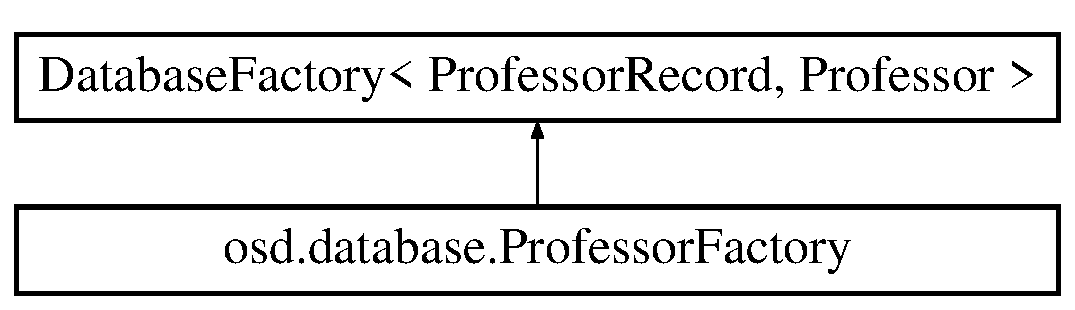
\includegraphics[height=2.000000cm]{classosd_1_1database_1_1_professor_factory}
\end{center}
\end{figure}
\subsection*{Public Member Functions}
\begin{DoxyCompactItemize}
\item 
\hypertarget{classosd_1_1database_1_1_professor_factory_abc33e8884766fdda3c30737082d37db2}{\hyperlink{interfaceosd_1_1input_1_1_professor}{Professor} {\bfseries create} (final \hyperlink{classosd_1_1database_1_1_professor_record}{Professor\-Record} record)}\label{classosd_1_1database_1_1_professor_factory_abc33e8884766fdda3c30737082d37db2}

\end{DoxyCompactItemize}


The documentation for this class was generated from the following file\-:\begin{DoxyCompactItemize}
\item 
/home/travis/build/\-Open-\/\-Source-\/\-Software-\/\-Development/class-\/scheduler/java/src/main/java/osd/database/Professor\-Factory.\-java\end{DoxyCompactItemize}

\hypertarget{classosd_1_1database_1_1_professor_record}{\section{osd.\-database.\-Professor\-Record Class Reference}
\label{classosd_1_1database_1_1_professor_record}\index{osd.\-database.\-Professor\-Record@{osd.\-database.\-Professor\-Record}}
}


The documentation for this class was generated from the following file\-:\begin{DoxyCompactItemize}
\item 
/home/travis/build/\-Open-\/\-Source-\/\-Software-\/\-Development/class-\/scheduler/java/src/main/java/osd/database/Professor\-Record.\-java\end{DoxyCompactItemize}

\hypertarget{classosd_1_1util_1_1relation_1_1_relation_3_01_k_00_01_l_00_01_v_00_01_w_01_4}{\section{osd.\-util.\-relation.\-Relation$<$ K, L, V, W $>$ Class Reference}
\label{classosd_1_1util_1_1relation_1_1_relation_3_01_k_00_01_l_00_01_v_00_01_w_01_4}\index{osd.\-util.\-relation.\-Relation$<$ K, L, V, W $>$@{osd.\-util.\-relation.\-Relation$<$ K, L, V, W $>$}}
}
\subsection*{Public Member Functions}
\begin{DoxyCompactItemize}
\item 
boolean \hyperlink{classosd_1_1util_1_1relation_1_1_relation_3_01_k_00_01_l_00_01_v_00_01_w_01_4_a0fb60240f1e512b1a294d121369f2889}{is\-Empty} ()
\item 
abstract void \hyperlink{classosd_1_1util_1_1relation_1_1_relation_3_01_k_00_01_l_00_01_v_00_01_w_01_4_ac4f315e51beb01d03f41b04dcc26d08e}{add} (final K key, final V value)
\item 
abstract void \hyperlink{classosd_1_1util_1_1relation_1_1_relation_3_01_k_00_01_l_00_01_v_00_01_w_01_4_a12762a3cab5c2992fb4ba707dd7353de}{remove} (final K key, final V value)
\item 
abstract void \hyperlink{classosd_1_1util_1_1relation_1_1_relation_3_01_k_00_01_l_00_01_v_00_01_w_01_4_a18530eaa2e035ad2940cd724276d4645}{remove} (final K key)
\item 
W \hyperlink{classosd_1_1util_1_1relation_1_1_relation_3_01_k_00_01_l_00_01_v_00_01_w_01_4_aacda8aa86e25b21488c4f2b4f67f88fe}{get} (final K key)
\item 
W \hyperlink{classosd_1_1util_1_1relation_1_1_relation_3_01_k_00_01_l_00_01_v_00_01_w_01_4_a432a888f2e80c5ad876bbb52d2b726f3}{get\-Or\-Default} (final K key, final Supplier$<$ W $>$ default\-Supplier)
\item 
abstract Relation$<$ V, W, K, L $>$ \hyperlink{classosd_1_1util_1_1relation_1_1_relation_3_01_k_00_01_l_00_01_v_00_01_w_01_4_ae94126ee35d81ad47715ab7db282b7e3}{reversed} ()
\item 
\hypertarget{classosd_1_1util_1_1relation_1_1_relation_3_01_k_00_01_l_00_01_v_00_01_w_01_4_a83ac26a5d528be62427b62f765db8424}{String {\bfseries to\-String} ()}\label{classosd_1_1util_1_1relation_1_1_relation_3_01_k_00_01_l_00_01_v_00_01_w_01_4_a83ac26a5d528be62427b62f765db8424}

\end{DoxyCompactItemize}
\subsection*{Protected Attributes}
\begin{DoxyCompactItemize}
\item 
final Map$<$ K, W $>$ \hyperlink{classosd_1_1util_1_1relation_1_1_relation_3_01_k_00_01_l_00_01_v_00_01_w_01_4_ae599c04310669afbba36859aa6f1531c}{forward}
\item 
final Map$<$ V, L $>$ \hyperlink{classosd_1_1util_1_1relation_1_1_relation_3_01_k_00_01_l_00_01_v_00_01_w_01_4_abaaa8f417c5097dd8b59141311170444}{reverse}
\end{DoxyCompactItemize}


\subsection{Detailed Description}
A reversible relation. Relations come in four flavors\-: 
\begin{DoxyItemize}
\item One-\/to-\/one, 
\item One-\/to-\/many, 
\item Many-\/to-\/one, 
\item Many-\/to-\/many. 
\end{DoxyItemize}The relation enforces these constraints, as appropriate. For example, a one-\/to-\/many relation will allow the same key to be associated with many values. However, if a second key would be associated with a value, the former key is first disassociated. 

One-\/to-\/many and many-\/to-\/many relations return their values as sets of whatever the value type is. One-\/to-\/one and many-\/to-\/one relations don't need to, and return instances of the value type directly. If a key isn't associated with anything,
\begin{DoxyCode}
null 
\end{DoxyCode}
 is returned to indicate this (if the relationship is one-\/to-\/many or many-\/to-\/many, a lookup will {\itshape never} return an empty set.

All four kinds of relations can be reversed, yielding a new relation whose values are the keys of the original, and whose keys are its values. One-\/to-\/many and many-\/to-\/one relations reverse to each other.


\begin{DoxyParams}{Parameters}
{\em $<$\-K$>$} & the type of key \\
\hline
{\em $<$\-L$>$} & either K (one-\/to-\/one or one-\/to-\/many) or
\begin{DoxyCode}
Set<K> 
\end{DoxyCode}
 (otherwise) \\
\hline
{\em $<$\-V$>$} & the type of value \\
\hline
{\em $<$\-W$>$} & either V (one-\/to-\/one or many-\/to-\/one) or
\begin{DoxyCode}
Set<V> 
\end{DoxyCode}
 (otherwise) \\
\hline
\end{DoxyParams}


\subsection{Member Function Documentation}
\hypertarget{classosd_1_1util_1_1relation_1_1_relation_3_01_k_00_01_l_00_01_v_00_01_w_01_4_ac4f315e51beb01d03f41b04dcc26d08e}{\index{osd\-::util\-::relation\-::\-Relation$<$ K, L, V, W $>$@{osd\-::util\-::relation\-::\-Relation$<$ K, L, V, W $>$}!add@{add}}
\index{add@{add}!osd::util::relation::Relation< K, L, V, W >@{osd\-::util\-::relation\-::\-Relation$<$ K, L, V, W $>$}}
\subsubsection[{add}]{\setlength{\rightskip}{0pt plus 5cm}abstract void osd.\-util.\-relation.\-Relation$<$ K, L, V, W $>$.add (
\begin{DoxyParamCaption}
\item[{final K}]{key, }
\item[{final V}]{value}
\end{DoxyParamCaption}
)\hspace{0.3cm}{\ttfamily [abstract]}}}\label{classosd_1_1util_1_1relation_1_1_relation_3_01_k_00_01_l_00_01_v_00_01_w_01_4_ac4f315e51beb01d03f41b04dcc26d08e}
Associates a key and a value. If this relation is one-\/to-\/one or one-\/to-\/many, any previous associations to the given value are removed. Likewise, if this relation is one-\/to-\/one or many-\/to-\/one, any previous associations from that key are removed. 
\begin{DoxyParams}{Parameters}
{\em key} & the key to associate with a new value \\
\hline
{\em value} & the value to associate with a new key \\
\hline
\end{DoxyParams}
\hypertarget{classosd_1_1util_1_1relation_1_1_relation_3_01_k_00_01_l_00_01_v_00_01_w_01_4_aacda8aa86e25b21488c4f2b4f67f88fe}{\index{osd\-::util\-::relation\-::\-Relation$<$ K, L, V, W $>$@{osd\-::util\-::relation\-::\-Relation$<$ K, L, V, W $>$}!get@{get}}
\index{get@{get}!osd::util::relation::Relation< K, L, V, W >@{osd\-::util\-::relation\-::\-Relation$<$ K, L, V, W $>$}}
\subsubsection[{get}]{\setlength{\rightskip}{0pt plus 5cm}W osd.\-util.\-relation.\-Relation$<$ K, L, V, W $>$.get (
\begin{DoxyParamCaption}
\item[{final K}]{key}
\end{DoxyParamCaption}
)\hspace{0.3cm}{\ttfamily [inline]}}}\label{classosd_1_1util_1_1relation_1_1_relation_3_01_k_00_01_l_00_01_v_00_01_w_01_4_aacda8aa86e25b21488c4f2b4f67f88fe}
Gets the value(s) a key is associated with. If this relation is one-\/to-\/many or many-\/to-\/many, this returns a \hyperlink{}{java.\-util.\-Set} of the appropriate value type. Otherwise, it returns a single value. If the key is absent, this always returns
\begin{DoxyCode}
null 
\end{DoxyCode}
 . 

If a set is returned, it will support mutation operations, but modifications to that set will {\itshape not} write through to the relation, nor will changes to the relation be reflected in the set. This method will never return an empty set.

To 


\begin{DoxyParams}{Parameters}
{\em key} & the key to get values for \\
\hline
\end{DoxyParams}
\begin{DoxyReturn}{Returns}
the value or set of values 
\end{DoxyReturn}
\begin{DoxySeeAlso}{See Also}
Relation\-::reversed() 
\end{DoxySeeAlso}
\hypertarget{classosd_1_1util_1_1relation_1_1_relation_3_01_k_00_01_l_00_01_v_00_01_w_01_4_a432a888f2e80c5ad876bbb52d2b726f3}{\index{osd\-::util\-::relation\-::\-Relation$<$ K, L, V, W $>$@{osd\-::util\-::relation\-::\-Relation$<$ K, L, V, W $>$}!get\-Or\-Default@{get\-Or\-Default}}
\index{get\-Or\-Default@{get\-Or\-Default}!osd::util::relation::Relation< K, L, V, W >@{osd\-::util\-::relation\-::\-Relation$<$ K, L, V, W $>$}}
\subsubsection[{get\-Or\-Default}]{\setlength{\rightskip}{0pt plus 5cm}W osd.\-util.\-relation.\-Relation$<$ K, L, V, W $>$.get\-Or\-Default (
\begin{DoxyParamCaption}
\item[{final K}]{key, }
\item[{final Supplier$<$ W $>$}]{default\-Supplier}
\end{DoxyParamCaption}
)\hspace{0.3cm}{\ttfamily [inline]}}}\label{classosd_1_1util_1_1relation_1_1_relation_3_01_k_00_01_l_00_01_v_00_01_w_01_4_a432a888f2e80c5ad876bbb52d2b726f3}
Gets the value(s) a key is associated with, or a default. If the key is present, it is returned as with \hyperlink{}{get(\-Object)}. Otherwise, the provided \hyperlink{}{Supplier} is invoked to get a default, which is returned. This is most useful for $\ast$-\/to-\/many relations, where 
\begin{DoxyCode}
Collections::emptySet 
\end{DoxyCode}
 may be given if an empty set is desired instead of
\begin{DoxyCode}
null 
\end{DoxyCode}
 . 
\begin{DoxyParams}{Parameters}
{\em key} & the key to get values for \\
\hline
{\em default\-Supplier} & a supplier for default values \\
\hline
\end{DoxyParams}
\begin{DoxyReturn}{Returns}
the value or set of values, or the default 
\end{DoxyReturn}
\begin{DoxySeeAlso}{See Also}
java.\-util.\-Collections\-::empty\-Set() 
\end{DoxySeeAlso}
\hypertarget{classosd_1_1util_1_1relation_1_1_relation_3_01_k_00_01_l_00_01_v_00_01_w_01_4_a0fb60240f1e512b1a294d121369f2889}{\index{osd\-::util\-::relation\-::\-Relation$<$ K, L, V, W $>$@{osd\-::util\-::relation\-::\-Relation$<$ K, L, V, W $>$}!is\-Empty@{is\-Empty}}
\index{is\-Empty@{is\-Empty}!osd::util::relation::Relation< K, L, V, W >@{osd\-::util\-::relation\-::\-Relation$<$ K, L, V, W $>$}}
\subsubsection[{is\-Empty}]{\setlength{\rightskip}{0pt plus 5cm}boolean osd.\-util.\-relation.\-Relation$<$ K, L, V, W $>$.is\-Empty (
\begin{DoxyParamCaption}
{}
\end{DoxyParamCaption}
)\hspace{0.3cm}{\ttfamily [inline]}}}\label{classosd_1_1util_1_1relation_1_1_relation_3_01_k_00_01_l_00_01_v_00_01_w_01_4_a0fb60240f1e512b1a294d121369f2889}
Checks if this relation is empty. That is, if this return
\begin{DoxyCode}
\textcolor{keyword}{true} 
\end{DoxyCode}
 , it is impossible for a call to \hyperlink{}{get(\-Object)} to return non-\/
\begin{DoxyCode}
null 
\end{DoxyCode}
 . \begin{DoxyReturn}{Returns}
whether this relation is empty 
\end{DoxyReturn}
\hypertarget{classosd_1_1util_1_1relation_1_1_relation_3_01_k_00_01_l_00_01_v_00_01_w_01_4_a12762a3cab5c2992fb4ba707dd7353de}{\index{osd\-::util\-::relation\-::\-Relation$<$ K, L, V, W $>$@{osd\-::util\-::relation\-::\-Relation$<$ K, L, V, W $>$}!remove@{remove}}
\index{remove@{remove}!osd::util::relation::Relation< K, L, V, W >@{osd\-::util\-::relation\-::\-Relation$<$ K, L, V, W $>$}}
\subsubsection[{remove}]{\setlength{\rightskip}{0pt plus 5cm}abstract void osd.\-util.\-relation.\-Relation$<$ K, L, V, W $>$.remove (
\begin{DoxyParamCaption}
\item[{final K}]{key, }
\item[{final V}]{value}
\end{DoxyParamCaption}
)\hspace{0.3cm}{\ttfamily [abstract]}}}\label{classosd_1_1util_1_1relation_1_1_relation_3_01_k_00_01_l_00_01_v_00_01_w_01_4_a12762a3cab5c2992fb4ba707dd7353de}
Disassociates a key and a value. If they were previously associated, this has no effect. Otherwise, they are no longer associated. 
\begin{DoxyParams}{Parameters}
{\em key} & the key to disassociate from a value \\
\hline
{\em value} & the value to disassociate from a key \\
\hline
\end{DoxyParams}
\hypertarget{classosd_1_1util_1_1relation_1_1_relation_3_01_k_00_01_l_00_01_v_00_01_w_01_4_a18530eaa2e035ad2940cd724276d4645}{\index{osd\-::util\-::relation\-::\-Relation$<$ K, L, V, W $>$@{osd\-::util\-::relation\-::\-Relation$<$ K, L, V, W $>$}!remove@{remove}}
\index{remove@{remove}!osd::util::relation::Relation< K, L, V, W >@{osd\-::util\-::relation\-::\-Relation$<$ K, L, V, W $>$}}
\subsubsection[{remove}]{\setlength{\rightskip}{0pt plus 5cm}abstract void osd.\-util.\-relation.\-Relation$<$ K, L, V, W $>$.remove (
\begin{DoxyParamCaption}
\item[{final K}]{key}
\end{DoxyParamCaption}
)\hspace{0.3cm}{\ttfamily [abstract]}}}\label{classosd_1_1util_1_1relation_1_1_relation_3_01_k_00_01_l_00_01_v_00_01_w_01_4_a18530eaa2e035ad2940cd724276d4645}
Disassociates a key from any values it's associated with. 
\begin{DoxyParams}{Parameters}
{\em key} & the key to disassociate from all values \\
\hline
\end{DoxyParams}
\begin{DoxySeeAlso}{See Also}
Relation\-::reversed() 
\end{DoxySeeAlso}
\hypertarget{classosd_1_1util_1_1relation_1_1_relation_3_01_k_00_01_l_00_01_v_00_01_w_01_4_ae94126ee35d81ad47715ab7db282b7e3}{\index{osd\-::util\-::relation\-::\-Relation$<$ K, L, V, W $>$@{osd\-::util\-::relation\-::\-Relation$<$ K, L, V, W $>$}!reversed@{reversed}}
\index{reversed@{reversed}!osd::util::relation::Relation< K, L, V, W >@{osd\-::util\-::relation\-::\-Relation$<$ K, L, V, W $>$}}
\subsubsection[{reversed}]{\setlength{\rightskip}{0pt plus 5cm}abstract Relation$<$V, W, K, L$>$ osd.\-util.\-relation.\-Relation$<$ K, L, V, W $>$.reversed (
\begin{DoxyParamCaption}
{}
\end{DoxyParamCaption}
)\hspace{0.3cm}{\ttfamily [abstract]}}}\label{classosd_1_1util_1_1relation_1_1_relation_3_01_k_00_01_l_00_01_v_00_01_w_01_4_ae94126ee35d81ad47715ab7db282b7e3}
Gets a backwards view of this relation. If this relation is one-\/to-\/many, the view is many-\/to-\/one, and vice-\/verse. If it is one-\/to-\/one or many-\/to-\/many, the view has the same cardinality. Changes to the view write through to the original relation, and vice-\/verse. Since the keys and values are interchanged in the view, this is particularly useful for getting the key(s) associated with a value, or with the single-\/argument form of \hyperlink{}{remove(\-Object)}. \begin{DoxyReturn}{Returns}
a reversed view of this relation 
\end{DoxyReturn}


\subsection{Member Data Documentation}
\hypertarget{classosd_1_1util_1_1relation_1_1_relation_3_01_k_00_01_l_00_01_v_00_01_w_01_4_ae599c04310669afbba36859aa6f1531c}{\index{osd\-::util\-::relation\-::\-Relation$<$ K, L, V, W $>$@{osd\-::util\-::relation\-::\-Relation$<$ K, L, V, W $>$}!forward@{forward}}
\index{forward@{forward}!osd::util::relation::Relation< K, L, V, W >@{osd\-::util\-::relation\-::\-Relation$<$ K, L, V, W $>$}}
\subsubsection[{forward}]{\setlength{\rightskip}{0pt plus 5cm}final Map$<$K, W$>$ osd.\-util.\-relation.\-Relation$<$ K, L, V, W $>$.forward\hspace{0.3cm}{\ttfamily [protected]}}}\label{classosd_1_1util_1_1relation_1_1_relation_3_01_k_00_01_l_00_01_v_00_01_w_01_4_ae599c04310669afbba36859aa6f1531c}
This relation's data, in \char`\"{}forward\char`\"{} order. This map supports mutation operations, but be {\bfseries very careful} using them! It is recommended to use the methods of
\begin{DoxyCode}
Relation 
\end{DoxyCode}
 to avoid misaligned data. \hypertarget{classosd_1_1util_1_1relation_1_1_relation_3_01_k_00_01_l_00_01_v_00_01_w_01_4_abaaa8f417c5097dd8b59141311170444}{\index{osd\-::util\-::relation\-::\-Relation$<$ K, L, V, W $>$@{osd\-::util\-::relation\-::\-Relation$<$ K, L, V, W $>$}!reverse@{reverse}}
\index{reverse@{reverse}!osd::util::relation::Relation< K, L, V, W >@{osd\-::util\-::relation\-::\-Relation$<$ K, L, V, W $>$}}
\subsubsection[{reverse}]{\setlength{\rightskip}{0pt plus 5cm}final Map$<$V, L$>$ osd.\-util.\-relation.\-Relation$<$ K, L, V, W $>$.reverse\hspace{0.3cm}{\ttfamily [protected]}}}\label{classosd_1_1util_1_1relation_1_1_relation_3_01_k_00_01_l_00_01_v_00_01_w_01_4_abaaa8f417c5097dd8b59141311170444}
This relation's data, in \char`\"{}reverse\char`\"{} order. This map supports mutation operations, but be {\bfseries very careful} using them! It is recommended to use the methods of
\begin{DoxyCode}
Relation 
\end{DoxyCode}
 to avoid misaligned data. 

The documentation for this class was generated from the following file\-:\begin{DoxyCompactItemize}
\item 
/home/travis/build/\-Open-\/\-Source-\/\-Software-\/\-Development/class-\/scheduler/java/src/main/java/osd/util/relation/Relation.\-java\end{DoxyCompactItemize}

\hypertarget{interfaceosd_1_1output_1_1_results}{\section{osd.\-output.\-Results Interface Reference}
\label{interfaceosd_1_1output_1_1_results}\index{osd.\-output.\-Results@{osd.\-output.\-Results}}
}


Inherited by osd.\-schedule.\-Scheduler\-Results.

\subsection*{Public Member Functions}
\begin{DoxyCompactItemize}
\item 
List$<$ \hyperlink{classosd_1_1output_1_1_hunk}{Hunk} $>$ \hyperlink{interfaceosd_1_1output_1_1_results_ab3ba5d6fbb97e579c73f065a39eeba94}{get\-Hunks} ()
\item 
int \hyperlink{interfaceosd_1_1output_1_1_results_a6c75f1e38400b3b8c6173e8868a27c8f}{get\-Expected\-Hunk\-Count} ()
\item 
default double \hyperlink{interfaceosd_1_1output_1_1_results_a8d94342ed8cf15db06ad480a4be65732}{get\-Hunk\-Percentage} ()
\end{DoxyCompactItemize}


\subsection{Member Function Documentation}
\hypertarget{interfaceosd_1_1output_1_1_results_a6c75f1e38400b3b8c6173e8868a27c8f}{\index{osd\-::output\-::\-Results@{osd\-::output\-::\-Results}!get\-Expected\-Hunk\-Count@{get\-Expected\-Hunk\-Count}}
\index{get\-Expected\-Hunk\-Count@{get\-Expected\-Hunk\-Count}!osd::output::Results@{osd\-::output\-::\-Results}}
\subsubsection[{get\-Expected\-Hunk\-Count}]{\setlength{\rightskip}{0pt plus 5cm}int osd.\-output.\-Results.\-get\-Expected\-Hunk\-Count (
\begin{DoxyParamCaption}
{}
\end{DoxyParamCaption}
)}}\label{interfaceosd_1_1output_1_1_results_a6c75f1e38400b3b8c6173e8868a27c8f}
Get the count of how many hunks we expect to have. \begin{DoxyReturn}{Returns}
the count of how many hunks we expect to have 
\end{DoxyReturn}
\hypertarget{interfaceosd_1_1output_1_1_results_a8d94342ed8cf15db06ad480a4be65732}{\index{osd\-::output\-::\-Results@{osd\-::output\-::\-Results}!get\-Hunk\-Percentage@{get\-Hunk\-Percentage}}
\index{get\-Hunk\-Percentage@{get\-Hunk\-Percentage}!osd::output::Results@{osd\-::output\-::\-Results}}
\subsubsection[{get\-Hunk\-Percentage}]{\setlength{\rightskip}{0pt plus 5cm}default double osd.\-output.\-Results.\-get\-Hunk\-Percentage (
\begin{DoxyParamCaption}
{}
\end{DoxyParamCaption}
)\hspace{0.3cm}{\ttfamily [inline]}}}\label{interfaceosd_1_1output_1_1_results_a8d94342ed8cf15db06ad480a4be65732}
Compute the percentage of hunks generated successfully. \begin{DoxyReturn}{Returns}
the percentage of hunks generated successfully 
\end{DoxyReturn}
\hypertarget{interfaceosd_1_1output_1_1_results_ab3ba5d6fbb97e579c73f065a39eeba94}{\index{osd\-::output\-::\-Results@{osd\-::output\-::\-Results}!get\-Hunks@{get\-Hunks}}
\index{get\-Hunks@{get\-Hunks}!osd::output::Results@{osd\-::output\-::\-Results}}
\subsubsection[{get\-Hunks}]{\setlength{\rightskip}{0pt plus 5cm}List$<${\bf Hunk}$>$ osd.\-output.\-Results.\-get\-Hunks (
\begin{DoxyParamCaption}
{}
\end{DoxyParamCaption}
)}}\label{interfaceosd_1_1output_1_1_results_ab3ba5d6fbb97e579c73f065a39eeba94}
Get the list of all hunks generated so far. This list may be safely modified; modifications will not be reflected in the scheduler nor future calls to this method. \begin{DoxyReturn}{Returns}
the list of all hunks generated so far 
\end{DoxyReturn}


The documentation for this interface was generated from the following file\-:\begin{DoxyCompactItemize}
\item 
/home/travis/build/\-Open-\/\-Source-\/\-Software-\/\-Development/class-\/scheduler/java/src/main/java/osd/output/Results.\-java\end{DoxyCompactItemize}

\hypertarget{interfaceosd_1_1input_1_1_room}{\section{osd.\-input.\-Room Class Reference}
\label{interfaceosd_1_1input_1_1_room}\index{osd.\-input.\-Room@{osd.\-input.\-Room}}
}
Inheritance diagram for osd.\-input.\-Room\-:\begin{figure}[H]
\begin{center}
\leavevmode
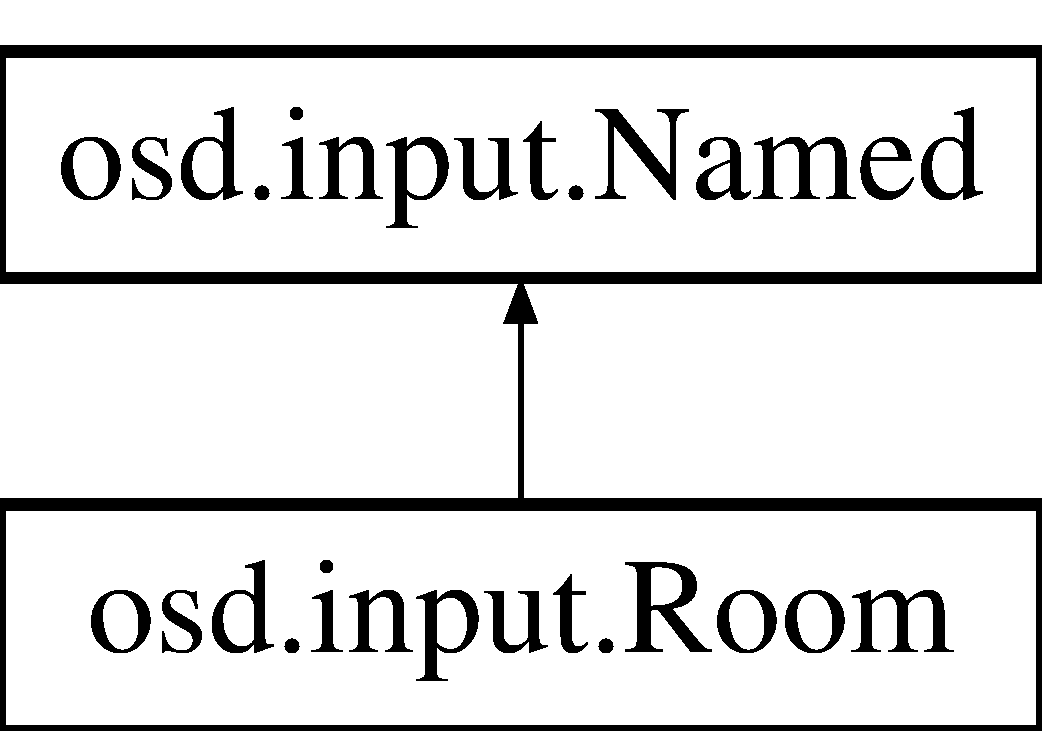
\includegraphics[height=2.000000cm]{interfaceosd_1_1input_1_1_room}
\end{center}
\end{figure}
\subsection*{Public Member Functions}
\begin{DoxyCompactItemize}
\item 
\hyperlink{interfaceosd_1_1input_1_1_room_type}{Room\-Type} \hyperlink{interfaceosd_1_1input_1_1_room_a45d616a99e600cd98fe09b7e654c1c71}{get\-Room\-Type} ()
\item 
\hypertarget{interfaceosd_1_1input_1_1_room_aff0170cca05e192a8d9d945d9c82f37c}{{\bfseries Room} (String t\-Building, int t\-Id, int t\-Capacity, \hyperlink{interfaceosd_1_1input_1_1_room_type}{Room\-Type} t\-Type, String t\-Division)}\label{interfaceosd_1_1input_1_1_room_aff0170cca05e192a8d9d945d9c82f37c}

\item 
\hypertarget{interfaceosd_1_1input_1_1_room_a1b6f1058bdfd643b5d457afdaee02b39}{String {\bfseries get\-Building} ()}\label{interfaceosd_1_1input_1_1_room_a1b6f1058bdfd643b5d457afdaee02b39}

\item 
\hypertarget{interfaceosd_1_1input_1_1_room_a3a1d32300a7e7224ff3b7a074a6d4f83}{String {\bfseries get\-Division} ()}\label{interfaceosd_1_1input_1_1_room_a3a1d32300a7e7224ff3b7a074a6d4f83}

\item 
\hypertarget{interfaceosd_1_1input_1_1_room_a9f436bfe04f749313d91c6be630d4df3}{int {\bfseries get\-Id} ()}\label{interfaceosd_1_1input_1_1_room_a9f436bfe04f749313d91c6be630d4df3}

\item 
\hypertarget{interfaceosd_1_1input_1_1_room_af906f320894f60f4f7fceb39bd85c3ba}{int {\bfseries get\-Capacity} ()}\label{interfaceosd_1_1input_1_1_room_af906f320894f60f4f7fceb39bd85c3ba}

\item 
\hypertarget{interfaceosd_1_1input_1_1_room_ae1888e550649197b473e98c38713ee53}{\hyperlink{interfaceosd_1_1input_1_1_room_type}{Room\-Type} {\bfseries get\-Type} ()}\label{interfaceosd_1_1input_1_1_room_ae1888e550649197b473e98c38713ee53}

\end{DoxyCompactItemize}


\subsection{Detailed Description}
Represents a specific room. 

\subsection{Member Function Documentation}
\hypertarget{interfaceosd_1_1input_1_1_room_a45d616a99e600cd98fe09b7e654c1c71}{\index{osd\-::input\-::\-Room@{osd\-::input\-::\-Room}!get\-Room\-Type@{get\-Room\-Type}}
\index{get\-Room\-Type@{get\-Room\-Type}!osd::input::Room@{osd\-::input\-::\-Room}}
\subsubsection[{get\-Room\-Type}]{\setlength{\rightskip}{0pt plus 5cm}{\bf Room\-Type} osd.\-input.\-Room.\-get\-Room\-Type (
\begin{DoxyParamCaption}
{}
\end{DoxyParamCaption}
)}}\label{interfaceosd_1_1input_1_1_room_a45d616a99e600cd98fe09b7e654c1c71}
Determines what type of room this is. \begin{DoxyReturn}{Returns}
what type of room this is 
\end{DoxyReturn}


The documentation for this class was generated from the following file\-:\begin{DoxyCompactItemize}
\item 
/home/travis/build/\-Open-\/\-Source-\/\-Software-\/\-Development/class-\/scheduler/java/src/main/java/osd/input/Room.\-java\end{DoxyCompactItemize}

\hypertarget{classroom__data_1_1models_1_1_room}{\section{room\-\_\-data.\-models.\-Room Class Reference}
\label{classroom__data_1_1models_1_1_room}\index{room\-\_\-data.\-models.\-Room@{room\-\_\-data.\-models.\-Room}}
}
Inheritance diagram for room\-\_\-data.\-models.\-Room\-:\begin{figure}[H]
\begin{center}
\leavevmode
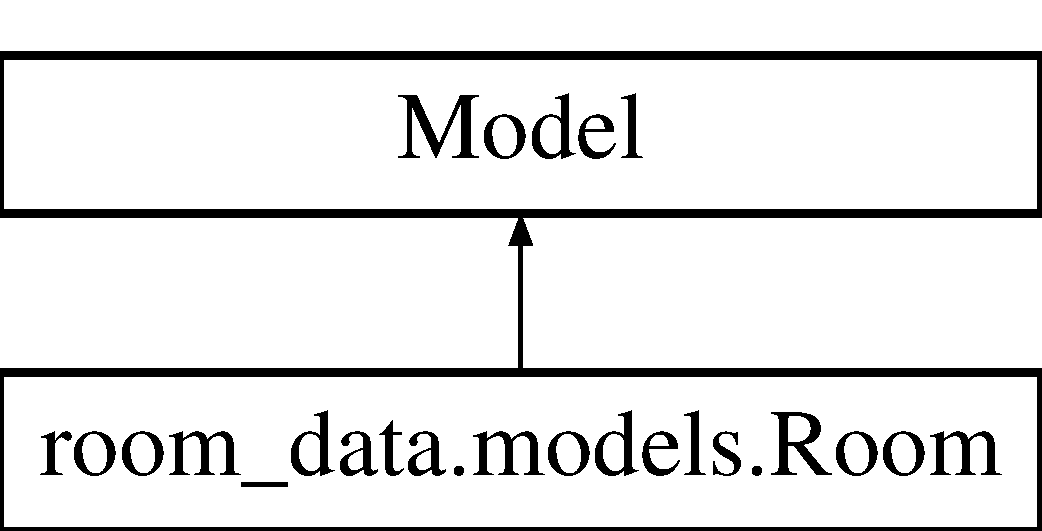
\includegraphics[height=2.000000cm]{classroom__data_1_1models_1_1_room}
\end{center}
\end{figure}
\subsection*{Public Member Functions}
\begin{DoxyCompactItemize}
\item 
\hypertarget{classroom__data_1_1models_1_1_room_adf410d3fb8402a17f0601568c781e33b}{def {\bfseries \-\_\-\-\_\-str\-\_\-\-\_\-}}\label{classroom__data_1_1models_1_1_room_adf410d3fb8402a17f0601568c781e33b}

\end{DoxyCompactItemize}
\subsection*{Static Public Attributes}
\begin{DoxyCompactItemize}
\item 
\hypertarget{classroom__data_1_1models_1_1_room_a84c6045cd2158c8f1f530787dbb6e04c}{tuple {\bfseries building} = models.\-Char\-Field(max\-\_\-length=20)}\label{classroom__data_1_1models_1_1_room_a84c6045cd2158c8f1f530787dbb6e04c}

\item 
\hypertarget{classroom__data_1_1models_1_1_room_a4465c5e69d8764d6351fd761c6976a23}{tuple {\bfseries room} = models.\-Char\-Field(max\-\_\-length=20)}\label{classroom__data_1_1models_1_1_room_a4465c5e69d8764d6351fd761c6976a23}

\item 
\hypertarget{classroom__data_1_1models_1_1_room_aaeb7b8d63866030db3056ebf684095fb}{tuple {\bfseries capacity} = models.\-Char\-Field(max\-\_\-length=20)}\label{classroom__data_1_1models_1_1_room_aaeb7b8d63866030db3056ebf684095fb}

\item 
\hypertarget{classroom__data_1_1models_1_1_room_a1f34c55b05bdc3d9b720462950b0a790}{tuple {\bfseries type\-\_\-room} = models.\-Char\-Field(max\-\_\-length=100)}\label{classroom__data_1_1models_1_1_room_a1f34c55b05bdc3d9b720462950b0a790}

\item 
\hypertarget{classroom__data_1_1models_1_1_room_a6afd19c6865edcd6fb71b0138ebbd503}{tuple {\bfseries division} = models.\-Char\-Field(max\-\_\-length=100)}\label{classroom__data_1_1models_1_1_room_a6afd19c6865edcd6fb71b0138ebbd503}

\item 
\hypertarget{classroom__data_1_1models_1_1_room_aa752bd2000141de26a99993b319f7b85}{tuple {\bfseries subject} = models.\-Char\-Field(max\-\_\-length=100)}\label{classroom__data_1_1models_1_1_room_aa752bd2000141de26a99993b319f7b85}

\item 
\hypertarget{classroom__data_1_1models_1_1_room_a3c131868dd4abf806b74c4f4fc27c564}{tuple {\bfseries course\-\_\-style} = models.\-Char\-Field(max\-\_\-length=100)}\label{classroom__data_1_1models_1_1_room_a3c131868dd4abf806b74c4f4fc27c564}

\end{DoxyCompactItemize}


The documentation for this class was generated from the following file\-:\begin{DoxyCompactItemize}
\item 
/home/travis/build/\-Open-\/\-Source-\/\-Software-\/\-Development/class-\/scheduler/mysite/room\-\_\-data/models.\-py\end{DoxyCompactItemize}

\hypertarget{classscheduler_1_1models_1_1_room}{\section{scheduler.\-models.\-Room Class Reference}
\label{classscheduler_1_1models_1_1_room}\index{scheduler.\-models.\-Room@{scheduler.\-models.\-Room}}
}
Inheritance diagram for scheduler.\-models.\-Room\-:\begin{figure}[H]
\begin{center}
\leavevmode
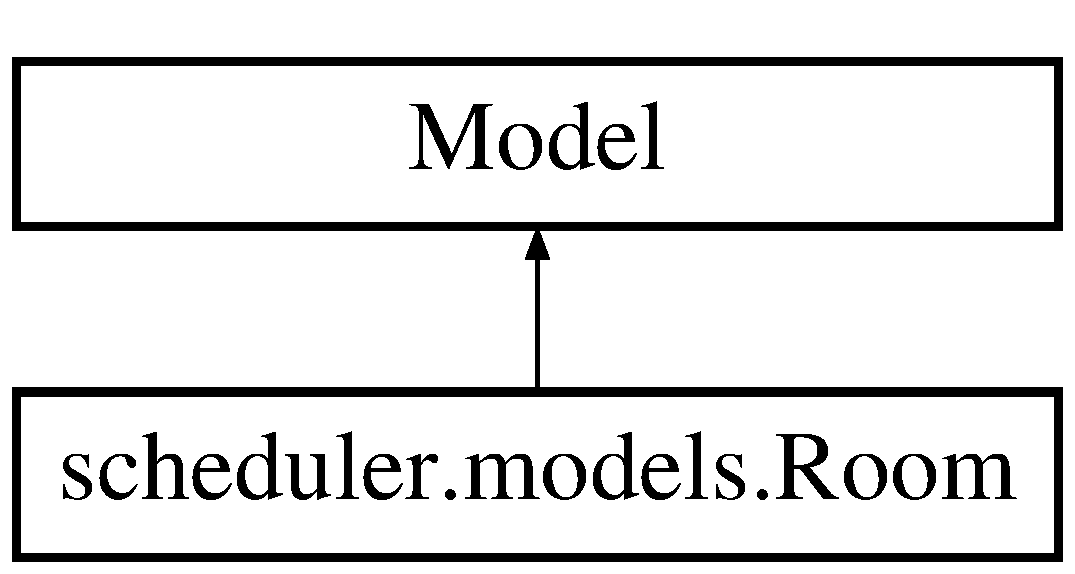
\includegraphics[height=3.000000cm]{classscheduler_1_1models_1_1_room}
\end{center}
\end{figure}
\subsection*{Static Public Attributes}
\begin{DoxyCompactItemize}
\item 
\hypertarget{classscheduler_1_1models_1_1_room_ae20a236603dca32bdaaad8e39c56f7ea}{tuple {\bfseries division} = models.\-Foreign\-Key(\hyperlink{classscheduler_1_1models_1_1_division}{Division}, on\-\_\-delete=models.\-C\-A\-S\-C\-A\-D\-E)}\label{classscheduler_1_1models_1_1_room_ae20a236603dca32bdaaad8e39c56f7ea}

\item 
\hypertarget{classscheduler_1_1models_1_1_room_ac160d40e28f0ce48c1b2843b225981ab}{tuple {\bfseries room\-\_\-type} = models.\-Foreign\-Key(\hyperlink{classscheduler_1_1models_1_1_room_type}{Room\-Type}, on\-\_\-delete=models.\-C\-A\-S\-C\-A\-D\-E)}\label{classscheduler_1_1models_1_1_room_ac160d40e28f0ce48c1b2843b225981ab}

\end{DoxyCompactItemize}
\subsection*{Additional Inherited Members}


The documentation for this class was generated from the following file\-:\begin{DoxyCompactItemize}
\item 
/home/travis/build/\-Open-\/\-Source-\/\-Software-\/\-Development/class-\/scheduler/mysite/scheduler/models.\-py\end{DoxyCompactItemize}

\hypertarget{classroom__data_1_1apps_1_1_room_data_config}{\section{room\-\_\-data.\-apps.\-Room\-Data\-Config Class Reference}
\label{classroom__data_1_1apps_1_1_room_data_config}\index{room\-\_\-data.\-apps.\-Room\-Data\-Config@{room\-\_\-data.\-apps.\-Room\-Data\-Config}}
}
Inheritance diagram for room\-\_\-data.\-apps.\-Room\-Data\-Config\-:\begin{figure}[H]
\begin{center}
\leavevmode
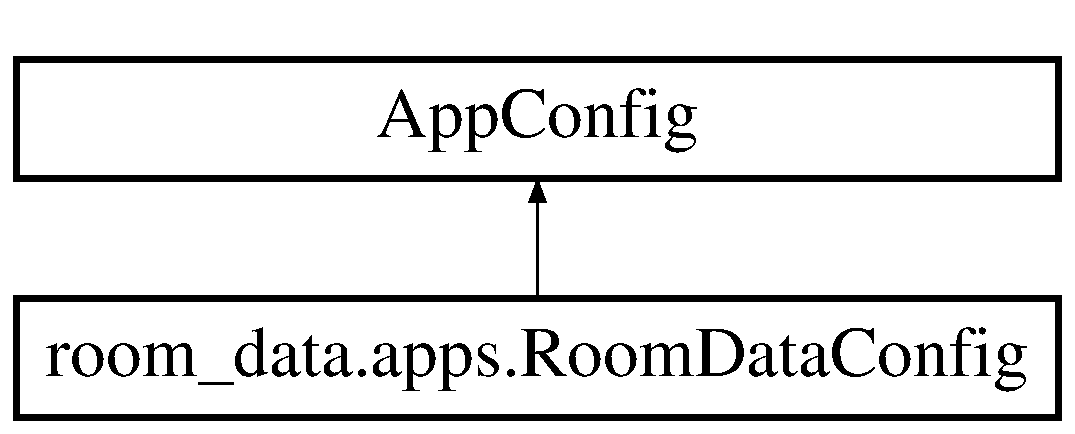
\includegraphics[height=2.000000cm]{classroom__data_1_1apps_1_1_room_data_config}
\end{center}
\end{figure}
\subsection*{Static Public Attributes}
\begin{DoxyCompactItemize}
\item 
\hypertarget{classroom__data_1_1apps_1_1_room_data_config_a1e3dda1d063b567cfe254041713219cf}{string {\bfseries name} = 'room\-\_\-data'}\label{classroom__data_1_1apps_1_1_room_data_config_a1e3dda1d063b567cfe254041713219cf}

\end{DoxyCompactItemize}


The documentation for this class was generated from the following file\-:\begin{DoxyCompactItemize}
\item 
/home/travis/build/\-Open-\/\-Source-\/\-Software-\/\-Development/class-\/scheduler/mysite/room\-\_\-data/apps.\-py\end{DoxyCompactItemize}

\hypertarget{classosd_1_1database_1_1_room_factory}{\section{osd.\-database.\-Room\-Factory Class Reference}
\label{classosd_1_1database_1_1_room_factory}\index{osd.\-database.\-Room\-Factory@{osd.\-database.\-Room\-Factory}}
}
Inheritance diagram for osd.\-database.\-Room\-Factory\-:\begin{figure}[H]
\begin{center}
\leavevmode
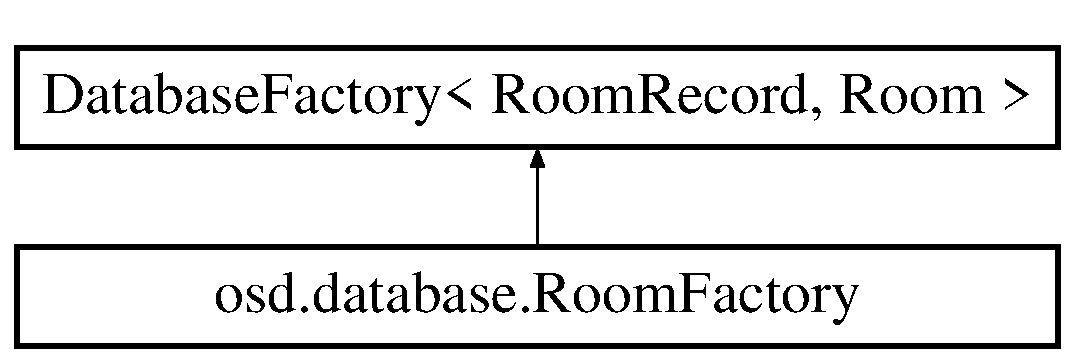
\includegraphics[height=2.000000cm]{classosd_1_1database_1_1_room_factory}
\end{center}
\end{figure}
\subsection*{Public Member Functions}
\begin{DoxyCompactItemize}
\item 
\hypertarget{classosd_1_1database_1_1_room_factory_a67be9e75d752fd52f9843c68b8b2d0b0}{\hyperlink{interfaceosd_1_1input_1_1_room}{Room} {\bfseries create} (final \hyperlink{classosd_1_1database_1_1_room_record}{Room\-Record} record)}\label{classosd_1_1database_1_1_room_factory_a67be9e75d752fd52f9843c68b8b2d0b0}

\end{DoxyCompactItemize}


The documentation for this class was generated from the following file\-:\begin{DoxyCompactItemize}
\item 
/home/travis/build/\-Open-\/\-Source-\/\-Software-\/\-Development/class-\/scheduler/java/src/main/java/osd/database/Room\-Factory.\-java\end{DoxyCompactItemize}

\hypertarget{classscheduler_1_1csv__parser_1_1_room_parser}{\section{scheduler.\-csv\-\_\-parser.\-Room\-Parser Class Reference}
\label{classscheduler_1_1csv__parser_1_1_room_parser}\index{scheduler.\-csv\-\_\-parser.\-Room\-Parser@{scheduler.\-csv\-\_\-parser.\-Room\-Parser}}
}
Inheritance diagram for scheduler.\-csv\-\_\-parser.\-Room\-Parser\-:\begin{figure}[H]
\begin{center}
\leavevmode
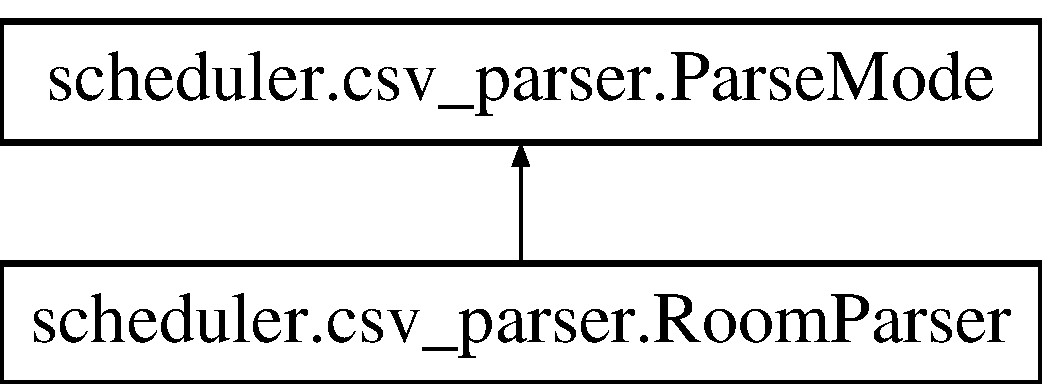
\includegraphics[height=2.000000cm]{classscheduler_1_1csv__parser_1_1_room_parser}
\end{center}
\end{figure}
\subsection*{Public Member Functions}
\begin{DoxyCompactItemize}
\item 
\hypertarget{classscheduler_1_1csv__parser_1_1_room_parser_a51d19b910c837d113ec19c65e8374da8}{def {\bfseries \-\_\-\-\_\-init\-\_\-\-\_\-}}\label{classscheduler_1_1csv__parser_1_1_room_parser_a51d19b910c837d113ec19c65e8374da8}

\item 
\hypertarget{classscheduler_1_1csv__parser_1_1_room_parser_a25e2ef8c3ff490928f6c3cffab628fbb}{def {\bfseries add\-\_\-row\-\_\-impl}}\label{classscheduler_1_1csv__parser_1_1_room_parser_a25e2ef8c3ff490928f6c3cffab628fbb}

\item 
\hypertarget{classscheduler_1_1csv__parser_1_1_room_parser_a3c5441a568b7a15955b351d0016e388f}{def {\bfseries get\-\_\-models}}\label{classscheduler_1_1csv__parser_1_1_room_parser_a3c5441a568b7a15955b351d0016e388f}

\end{DoxyCompactItemize}
\subsection*{Public Attributes}
\begin{DoxyCompactItemize}
\item 
\hypertarget{classscheduler_1_1csv__parser_1_1_room_parser_adcc8d7d3782ebaadbcc4ece558bf4fad}{{\bfseries rooms}}\label{classscheduler_1_1csv__parser_1_1_room_parser_adcc8d7d3782ebaadbcc4ece558bf4fad}

\item 
\hypertarget{classscheduler_1_1csv__parser_1_1_room_parser_a799d0bcbd8a603e56732004b84875a74}{{\bfseries room\-\_\-types}}\label{classscheduler_1_1csv__parser_1_1_room_parser_a799d0bcbd8a603e56732004b84875a74}

\end{DoxyCompactItemize}
\subsection*{Static Public Attributes}
\begin{DoxyCompactItemize}
\item 
\hypertarget{classscheduler_1_1csv__parser_1_1_room_parser_a032f2c787da1fa2509d92458b20b3456}{tuple {\bfseries columns} = (\char`\"{}building\char`\"{}, \char`\"{}room\char`\"{}, \char`\"{}type\char`\"{}, \char`\"{}division\char`\"{})}\label{classscheduler_1_1csv__parser_1_1_room_parser_a032f2c787da1fa2509d92458b20b3456}

\end{DoxyCompactItemize}


The documentation for this class was generated from the following file\-:\begin{DoxyCompactItemize}
\item 
/home/travis/build/\-Open-\/\-Source-\/\-Software-\/\-Development/class-\/scheduler/mysite/scheduler/csv\-\_\-parser.\-py\end{DoxyCompactItemize}

\hypertarget{classosd_1_1database_1_1_room_record}{\section{osd.\-database.\-Room\-Record Class Reference}
\label{classosd_1_1database_1_1_room_record}\index{osd.\-database.\-Room\-Record@{osd.\-database.\-Room\-Record}}
}


The documentation for this class was generated from the following file\-:\begin{DoxyCompactItemize}
\item 
/home/travis/build/\-Open-\/\-Source-\/\-Software-\/\-Development/class-\/scheduler/java/src/main/java/osd/database/Room\-Record.\-java\end{DoxyCompactItemize}

\hypertarget{interfaceosd_1_1input_1_1_room_type}{\section{osd.\-input.\-Room\-Type Class Reference}
\label{interfaceosd_1_1input_1_1_room_type}\index{osd.\-input.\-Room\-Type@{osd.\-input.\-Room\-Type}}
}
Inheritance diagram for osd.\-input.\-Room\-Type\-:\begin{figure}[H]
\begin{center}
\leavevmode
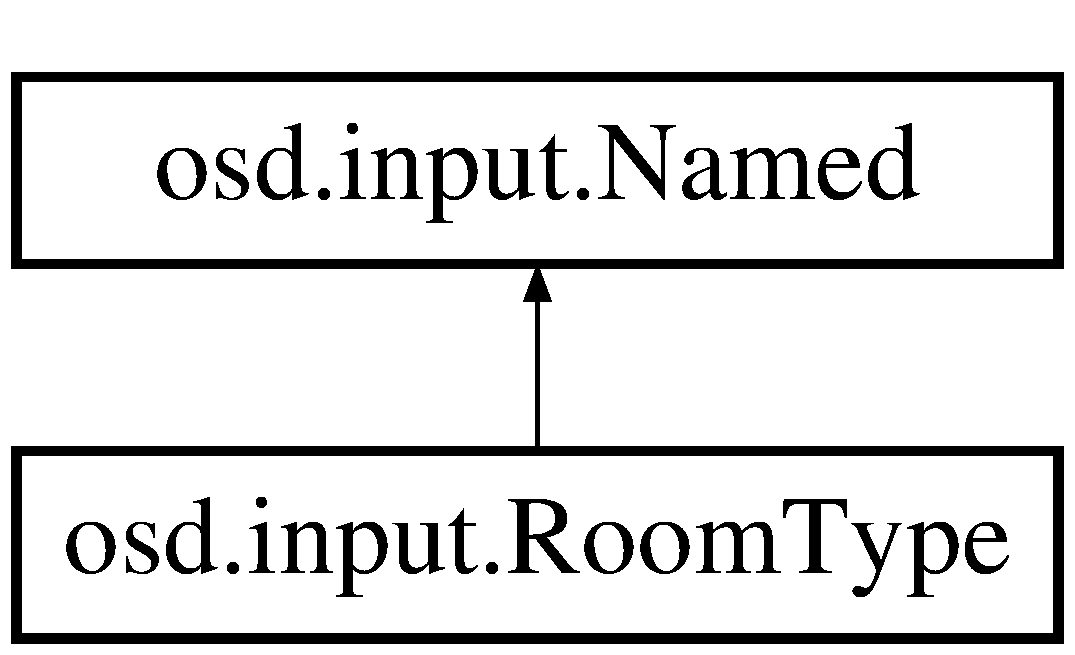
\includegraphics[height=2.000000cm]{interfaceosd_1_1input_1_1_room_type}
\end{center}
\end{figure}
\subsection*{Public Member Functions}
\begin{DoxyCompactItemize}
\item 
\hypertarget{interfaceosd_1_1input_1_1_room_type_a1424e5b21be64ec53e15a86bd3881786}{{\bfseries Room\-Type} (String t\-Name, int t\-Id)}\label{interfaceosd_1_1input_1_1_room_type_a1424e5b21be64ec53e15a86bd3881786}

\end{DoxyCompactItemize}


\subsection{Detailed Description}
Represents a type of room. Examples include \char`\"{}classroom\char`\"{}, \char`\"{}\-Windows lab\char`\"{}, and \char`\"{}darkroom\char`\"{}. 

The documentation for this class was generated from the following file\-:\begin{DoxyCompactItemize}
\item 
/home/travis/build/\-Open-\/\-Source-\/\-Software-\/\-Development/class-\/scheduler/java/src/main/java/osd/input/Room\-Type.\-java\end{DoxyCompactItemize}

\hypertarget{classscheduler_1_1models_1_1_room_type}{\section{scheduler.\-models.\-Room\-Type Class Reference}
\label{classscheduler_1_1models_1_1_room_type}\index{scheduler.\-models.\-Room\-Type@{scheduler.\-models.\-Room\-Type}}
}
Inheritance diagram for scheduler.\-models.\-Room\-Type\-:\begin{figure}[H]
\begin{center}
\leavevmode
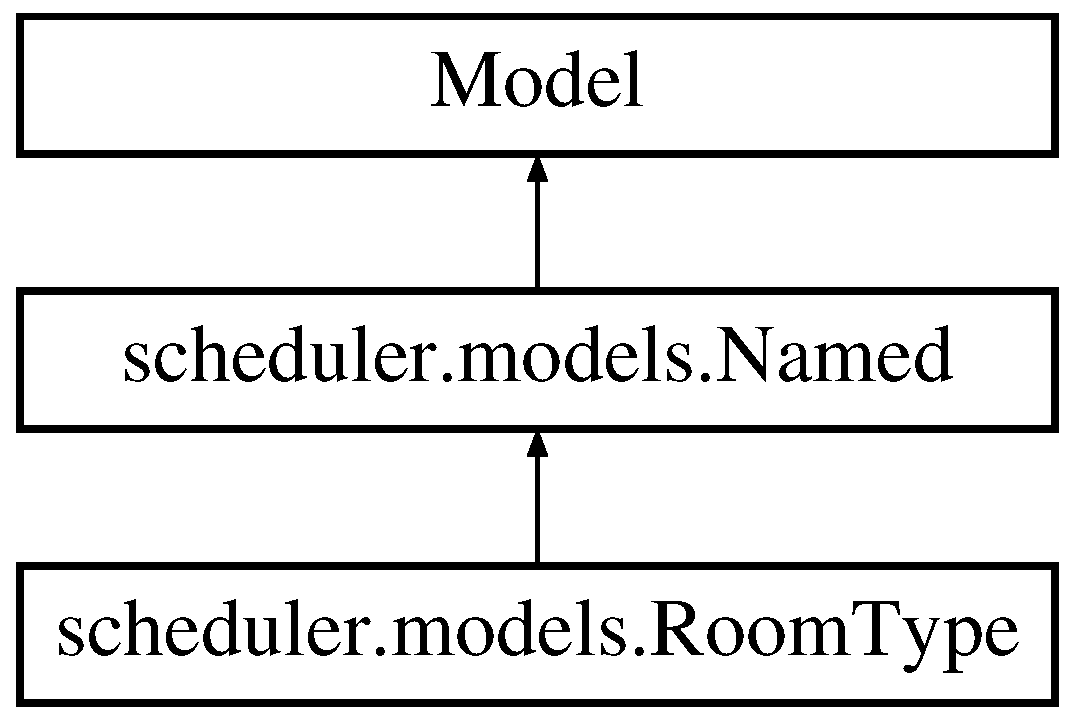
\includegraphics[height=3.000000cm]{classscheduler_1_1models_1_1_room_type}
\end{center}
\end{figure}
\subsection*{Additional Inherited Members}


The documentation for this class was generated from the following file\-:\begin{DoxyCompactItemize}
\item 
/home/travis/build/\-Open-\/\-Source-\/\-Software-\/\-Development/class-\/scheduler/mysite/scheduler/models.\-py\end{DoxyCompactItemize}

\hypertarget{classhibernate1_1_1_run_tables}{\section{hibernate1.\-Run\-Tables Class Reference}
\label{classhibernate1_1_1_run_tables}\index{hibernate1.\-Run\-Tables@{hibernate1.\-Run\-Tables}}
}
\subsection*{Static Public Member Functions}
\begin{DoxyCompactItemize}
\item 
\hypertarget{classhibernate1_1_1_run_tables_a2a5479797664047fda2ab3da9c216d8e}{static void {\bfseries main} (String\mbox{[}$\,$\mbox{]} args)}\label{classhibernate1_1_1_run_tables_a2a5479797664047fda2ab3da9c216d8e}

\end{DoxyCompactItemize}


The documentation for this class was generated from the following file\-:\begin{DoxyCompactItemize}
\item 
/home/travis/build/\-Open-\/\-Source-\/\-Software-\/\-Development/class-\/scheduler/hibernate\-Setup/src/hibernate1/Run\-Tables.\-java\end{DoxyCompactItemize}

\hypertarget{interfaceosd_1_1schedule_1_1_schedule_module}{\section{osd.\-schedule.\-Schedule\-Module Interface Reference}
\label{interfaceosd_1_1schedule_1_1_schedule_module}\index{osd.\-schedule.\-Schedule\-Module@{osd.\-schedule.\-Schedule\-Module}}
}
\subsection*{Public Member Functions}
\begin{DoxyCompactItemize}
\item 
\hypertarget{interfaceosd_1_1schedule_1_1_schedule_module_acd26a40a792b5b0b9f62a8c3896f8396}{\hyperlink{interfaceosd_1_1schedule_1_1_scheduler}{Scheduler} {\bfseries provides\-Scheduler} (Scheduler\-Impl impl)}\label{interfaceosd_1_1schedule_1_1_schedule_module_acd26a40a792b5b0b9f62a8c3896f8396}

\end{DoxyCompactItemize}


\subsection{Detailed Description}
Dagger module to provide the scheduler instance. 

The documentation for this interface was generated from the following file\-:\begin{DoxyCompactItemize}
\item 
/home/travis/build/\-Open-\/\-Source-\/\-Software-\/\-Development/class-\/scheduler/java/src/main/java/osd/schedule/Schedule\-Module.\-java\end{DoxyCompactItemize}

\hypertarget{interfaceosd_1_1schedule_1_1_scheduler}{\section{osd.\-schedule.\-Scheduler Interface Reference}
\label{interfaceosd_1_1schedule_1_1_scheduler}\index{osd.\-schedule.\-Scheduler@{osd.\-schedule.\-Scheduler}}
}


Inherited by osd.\-schedule.\-Scheduler\-Impl.

\subsection*{Public Member Functions}
\begin{DoxyCompactItemize}
\item 
boolean \hyperlink{interfaceosd_1_1schedule_1_1_scheduler_a129884a57f2bf02c446b18c88c3582a2}{run} (final \hyperlink{interfaceosd_1_1output_1_1_callbacks}{Callbacks} callbacks)
\end{DoxyCompactItemize}


\subsection{Detailed Description}
Schedule algorithm entry point. Runs the algorithm itself, accepting  Callbacks callbacks\} to handle successful and failed results. 

\subsection{Member Function Documentation}
\hypertarget{interfaceosd_1_1schedule_1_1_scheduler_a129884a57f2bf02c446b18c88c3582a2}{\index{osd\-::schedule\-::\-Scheduler@{osd\-::schedule\-::\-Scheduler}!run@{run}}
\index{run@{run}!osd::schedule::Scheduler@{osd\-::schedule\-::\-Scheduler}}
\subsubsection[{run}]{\setlength{\rightskip}{0pt plus 5cm}boolean osd.\-schedule.\-Scheduler.\-run (
\begin{DoxyParamCaption}
\item[{final {\bf Callbacks}}]{callbacks}
\end{DoxyParamCaption}
)}}\label{interfaceosd_1_1schedule_1_1_scheduler_a129884a57f2bf02c446b18c88c3582a2}
Runs the scheduler algorithm. The \hyperlink{}{Callbacks} argument customizes the scheduling behavior by providing a {\itshape stop condition} (eg. \char`\"{}run
until 5 schedules have been generated\char`\"{}) and output callbacks. The return value indicates whether the stop condition was actually met, or whether we ran out of candidates first. 
\begin{DoxyParams}{Parameters}
{\em callbacks} & callbacks for handling results \\
\hline
\end{DoxyParams}
\begin{DoxyReturn}{Returns}
whether we met the stop condition before running out of candidates 
\end{DoxyReturn}


The documentation for this interface was generated from the following file\-:\begin{DoxyCompactItemize}
\item 
/home/travis/build/\-Open-\/\-Source-\/\-Software-\/\-Development/class-\/scheduler/java/src/main/java/osd/schedule/Scheduler.\-java\end{DoxyCompactItemize}

\hypertarget{classscheduler_1_1apps_1_1_scheduler_config}{\section{scheduler.\-apps.\-Scheduler\-Config Class Reference}
\label{classscheduler_1_1apps_1_1_scheduler_config}\index{scheduler.\-apps.\-Scheduler\-Config@{scheduler.\-apps.\-Scheduler\-Config}}
}
Inheritance diagram for scheduler.\-apps.\-Scheduler\-Config\-:\begin{figure}[H]
\begin{center}
\leavevmode
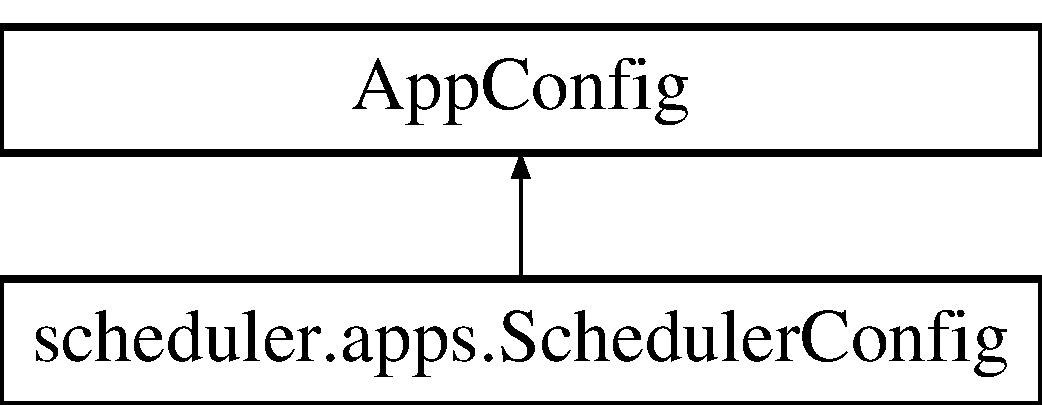
\includegraphics[height=2.000000cm]{classscheduler_1_1apps_1_1_scheduler_config}
\end{center}
\end{figure}
\subsection*{Static Public Attributes}
\begin{DoxyCompactItemize}
\item 
\hypertarget{classscheduler_1_1apps_1_1_scheduler_config_aebb64410f42031cde5364a964e8c85b3}{string {\bfseries name} = 'scheduler'}\label{classscheduler_1_1apps_1_1_scheduler_config_aebb64410f42031cde5364a964e8c85b3}

\end{DoxyCompactItemize}


The documentation for this class was generated from the following file\-:\begin{DoxyCompactItemize}
\item 
/home/travis/build/\-Open-\/\-Source-\/\-Software-\/\-Development/class-\/scheduler/mysite/scheduler/apps.\-py\end{DoxyCompactItemize}

\hypertarget{interfaceosd_1_1main_1_1_scheduling}{\section{osd.\-main.\-Scheduling Interface Reference}
\label{interfaceosd_1_1main_1_1_scheduling}\index{osd.\-main.\-Scheduling@{osd.\-main.\-Scheduling}}
}
\subsection*{Public Member Functions}
\begin{DoxyCompactItemize}
\item 
\hypertarget{interfaceosd_1_1main_1_1_scheduling_af6bbed1016f5ec74748faa35699a6d2a}{\hyperlink{interfaceosd_1_1schedule_1_1_scheduler}{Scheduler} {\bfseries scheduling\-Attempt} ()}\label{interfaceosd_1_1main_1_1_scheduling_af6bbed1016f5ec74748faa35699a6d2a}

\end{DoxyCompactItemize}
\subsection*{Static Public Member Functions}
\begin{DoxyCompactItemize}
\item 
\hypertarget{interfaceosd_1_1main_1_1_scheduling_a269ef3f49be0d634e02d7215262d2b85}{static void {\bfseries main} (final String\mbox{[}$\,$\mbox{]} args)  throws Parse\-Exception }\label{interfaceosd_1_1main_1_1_scheduling_a269ef3f49be0d634e02d7215262d2b85}

\end{DoxyCompactItemize}


The documentation for this interface was generated from the following file\-:\begin{DoxyCompactItemize}
\item 
/home/travis/build/\-Open-\/\-Source-\/\-Software-\/\-Development/class-\/scheduler/java/src/main/java/osd/main/Scheduling.\-java\end{DoxyCompactItemize}

\hypertarget{classscheduler_1_1models_1_1_section}{\section{scheduler.\-models.\-Section Class Reference}
\label{classscheduler_1_1models_1_1_section}\index{scheduler.\-models.\-Section@{scheduler.\-models.\-Section}}
}
Inheritance diagram for scheduler.\-models.\-Section\-:\begin{figure}[H]
\begin{center}
\leavevmode
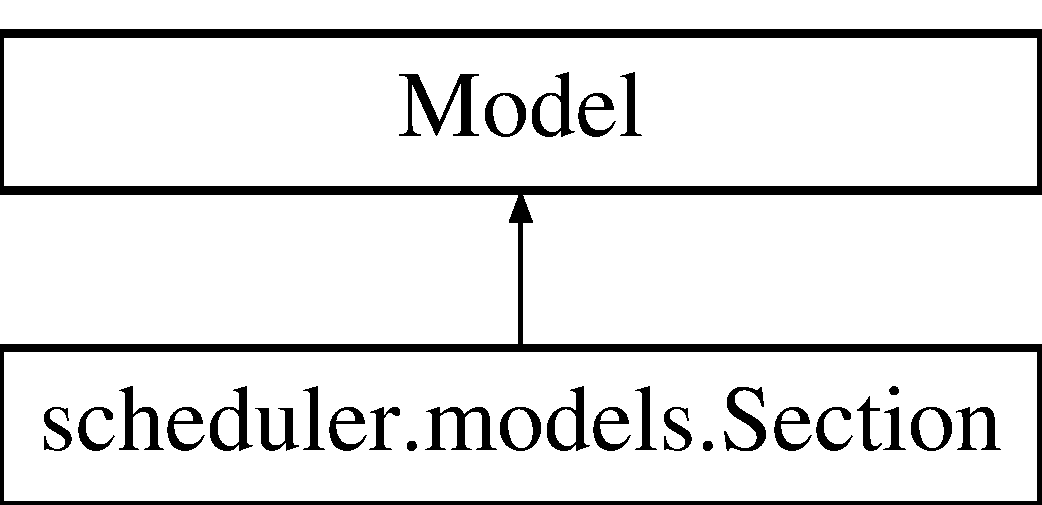
\includegraphics[height=2.000000cm]{classscheduler_1_1models_1_1_section}
\end{center}
\end{figure}
\subsection*{Public Member Functions}
\begin{DoxyCompactItemize}
\item 
\hypertarget{classscheduler_1_1models_1_1_section_a246a1f55dd3ce2f8b7e22b381535e09d}{def {\bfseries \-\_\-\-\_\-str\-\_\-\-\_\-}}\label{classscheduler_1_1models_1_1_section_a246a1f55dd3ce2f8b7e22b381535e09d}

\end{DoxyCompactItemize}
\subsection*{Static Public Attributes}
\begin{DoxyCompactItemize}
\item 
\hypertarget{classscheduler_1_1models_1_1_section_ac4fd835769f6add9617f8885b0d225fe}{tuple {\bfseries course} = models.\-Foreign\-Key(\hyperlink{classscheduler_1_1models_1_1_course}{Course}, on\-\_\-delete=models.\-C\-A\-S\-C\-A\-D\-E)}\label{classscheduler_1_1models_1_1_section_ac4fd835769f6add9617f8885b0d225fe}

\item 
\hypertarget{classscheduler_1_1models_1_1_section_a7cddf1d09f1567eb46674001375767b7}{tuple {\bfseries suffix} = models.\-Char\-Field(max\-\_\-length=50)}\label{classscheduler_1_1models_1_1_section_a7cddf1d09f1567eb46674001375767b7}

\end{DoxyCompactItemize}


The documentation for this class was generated from the following file\-:\begin{DoxyCompactItemize}
\item 
/home/travis/build/\-Open-\/\-Source-\/\-Software-\/\-Development/class-\/scheduler/mysite/scheduler/models.\-py\end{DoxyCompactItemize}

\hypertarget{interfaceosd_1_1input_1_1_section}{\section{osd.\-input.\-Section Class Reference}
\label{interfaceosd_1_1input_1_1_section}\index{osd.\-input.\-Section@{osd.\-input.\-Section}}
}
Inheritance diagram for osd.\-input.\-Section\-:\begin{figure}[H]
\begin{center}
\leavevmode
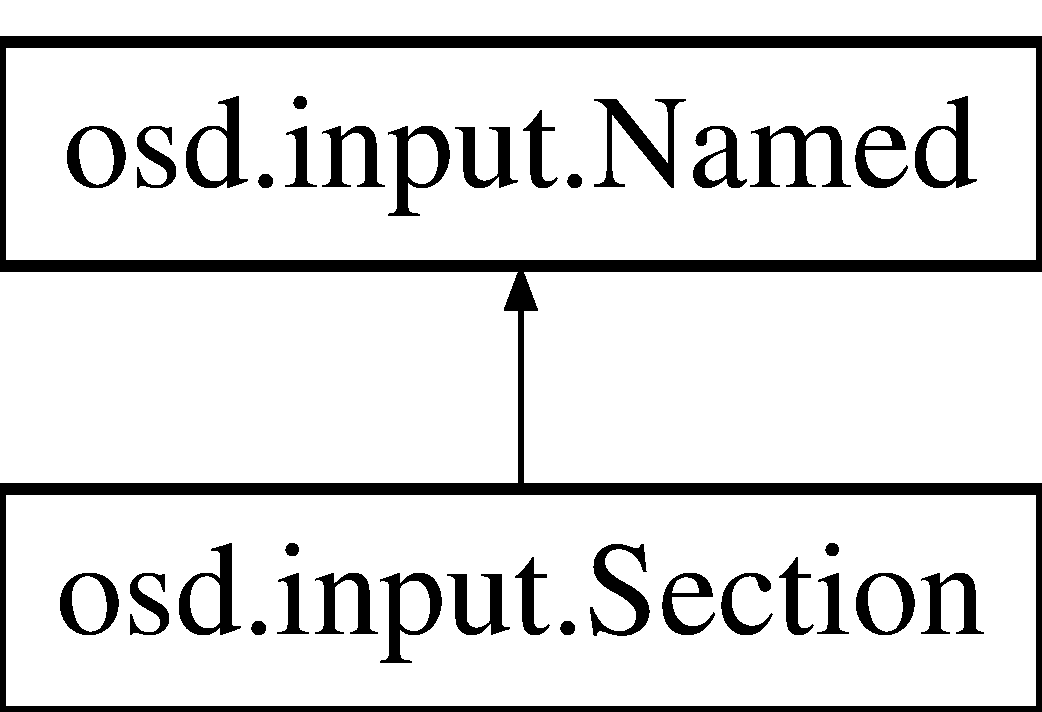
\includegraphics[height=2.000000cm]{interfaceosd_1_1input_1_1_section}
\end{center}
\end{figure}
\subsection*{Public Member Functions}
\begin{DoxyCompactItemize}
\item 
\hypertarget{interfaceosd_1_1input_1_1_section_a2df3a415bc510373a07d41ecd82e2e8e}{\hyperlink{interfaceosd_1_1input_1_1_course}{Course} {\bfseries get\-Course} ()}\label{interfaceosd_1_1input_1_1_section_a2df3a415bc510373a07d41ecd82e2e8e}

\item 
\hypertarget{interfaceosd_1_1input_1_1_section_a6a2334ee4c53a32f34b780b6e451aaca}{{\bfseries Section} (String t\-Course\-Id, String t\-Section\-Id, int t\-Capacity, \hyperlink{interfaceosd_1_1input_1_1_professor}{Professor} t\-Professor)}\label{interfaceosd_1_1input_1_1_section_a6a2334ee4c53a32f34b780b6e451aaca}

\item 
\hypertarget{interfaceosd_1_1input_1_1_section_af46be083d097979980bfd0b0f5107ad7}{String {\bfseries get\-Course\-Id} ()}\label{interfaceosd_1_1input_1_1_section_af46be083d097979980bfd0b0f5107ad7}

\item 
\hypertarget{interfaceosd_1_1input_1_1_section_a46b8bae68a9a19f6142aaf7b352cb9de}{String {\bfseries get\-Section\-Id} ()}\label{interfaceosd_1_1input_1_1_section_a46b8bae68a9a19f6142aaf7b352cb9de}

\item 
\hypertarget{interfaceosd_1_1input_1_1_section_ab9112a652964601ad4ca890a5f982b03}{int {\bfseries get\-Capacity} ()}\label{interfaceosd_1_1input_1_1_section_ab9112a652964601ad4ca890a5f982b03}

\item 
\hypertarget{interfaceosd_1_1input_1_1_section_a1d130811d59d44083852e3036d3e40dd}{\hyperlink{interfaceosd_1_1input_1_1_professor}{Professor} {\bfseries get\-Sec\-Professor} ()}\label{interfaceosd_1_1input_1_1_section_a1d130811d59d44083852e3036d3e40dd}

\end{DoxyCompactItemize}
\subsection*{Static Public Member Functions}
\begin{DoxyCompactItemize}
\item 
\hypertarget{interfaceosd_1_1input_1_1_section_a0f5625c7ae101d06636557b7e6a14e2a}{static \hyperlink{interfaceosd_1_1input_1_1_section}{Section} {\bfseries of} (final \hyperlink{interfaceosd_1_1input_1_1_course}{Course} course, final String suffix)}\label{interfaceosd_1_1input_1_1_section_a0f5625c7ae101d06636557b7e6a14e2a}

\end{DoxyCompactItemize}


\subsection{Detailed Description}
Represents a specific section of some course. 

The documentation for this class was generated from the following file\-:\begin{DoxyCompactItemize}
\item 
/home/travis/build/\-Open-\/\-Source-\/\-Software-\/\-Development/class-\/scheduler/java/src/main/java/osd/input/Section.\-java\end{DoxyCompactItemize}

\hypertarget{interfaceosd_1_1input_1_1_sources}{\section{osd.\-input.\-Sources Interface Reference}
\label{interfaceosd_1_1input_1_1_sources}\index{osd.\-input.\-Sources@{osd.\-input.\-Sources}}
}


Inherited by osd.\-input.\-placeholder.\-Placeholder\-Sources, and osd.\-input.\-Sources\-Impl.

\subsection*{Public Member Functions}
\begin{DoxyCompactItemize}
\item 
\hypertarget{interfaceosd_1_1input_1_1_sources_ad46d381ede2382bdc3d575b8fecd2c57}{Stream$<$ \hyperlink{interfaceosd_1_1input_1_1_section}{Section} $>$ {\bfseries get\-Sections} ()}\label{interfaceosd_1_1input_1_1_sources_ad46d381ede2382bdc3d575b8fecd2c57}

\item 
\hypertarget{interfaceosd_1_1input_1_1_sources_ae844eaa01c01072d29b5bed2b38ce93d}{Stream$<$ \hyperlink{interfaceosd_1_1input_1_1_professor}{Professor} $>$ {\bfseries get\-Professors} ()}\label{interfaceosd_1_1input_1_1_sources_ae844eaa01c01072d29b5bed2b38ce93d}

\item 
\hypertarget{interfaceosd_1_1input_1_1_sources_abf5eae21254e2e3ed7a117a3c9fa985b}{Stream$<$ \hyperlink{interfaceosd_1_1input_1_1_block}{Block} $>$ {\bfseries get\-Blocks} ()}\label{interfaceosd_1_1input_1_1_sources_abf5eae21254e2e3ed7a117a3c9fa985b}

\item 
\hypertarget{interfaceosd_1_1input_1_1_sources_ab8ee51527f51a8aa6c3179c93ac7466c}{Stream$<$ \hyperlink{interfaceosd_1_1input_1_1_room}{Room} $>$ {\bfseries get\-Rooms} ()}\label{interfaceosd_1_1input_1_1_sources_ab8ee51527f51a8aa6c3179c93ac7466c}

\end{DoxyCompactItemize}


The documentation for this interface was generated from the following file\-:\begin{DoxyCompactItemize}
\item 
/home/travis/build/\-Open-\/\-Source-\/\-Software-\/\-Development/class-\/scheduler/java/src/main/java/osd/input/Sources.\-java\end{DoxyCompactItemize}

\hypertarget{interfaceosd_1_1input_1_1_input_module_1_1_sources_module}{\section{osd.\-input.\-Input\-Module.\-Sources\-Module Interface Reference}
\label{interfaceosd_1_1input_1_1_input_module_1_1_sources_module}\index{osd.\-input.\-Input\-Module.\-Sources\-Module@{osd.\-input.\-Input\-Module.\-Sources\-Module}}
}
\subsection*{Public Member Functions}
\begin{DoxyCompactItemize}
\item 
\hypertarget{interfaceosd_1_1input_1_1_input_module_1_1_sources_module_ac480b8bb12fb70d405265f096d4dfd8f}{\hyperlink{interfaceosd_1_1input_1_1_sources}{Sources} {\bfseries sources\-Impl} (Sources\-Impl sources)}\label{interfaceosd_1_1input_1_1_input_module_1_1_sources_module_ac480b8bb12fb70d405265f096d4dfd8f}

\end{DoxyCompactItemize}


\subsection{Detailed Description}
Nested interface trick to use  alongside . 

The documentation for this interface was generated from the following file\-:\begin{DoxyCompactItemize}
\item 
/home/travis/build/\-Open-\/\-Source-\/\-Software-\/\-Development/class-\/scheduler/java/src/main/java/osd/input/Input\-Module.\-java\end{DoxyCompactItemize}

\hypertarget{classscheduler_1_1tests_1_1_test_models}{\section{scheduler.\-tests.\-Test\-Models Class Reference}
\label{classscheduler_1_1tests_1_1_test_models}\index{scheduler.\-tests.\-Test\-Models@{scheduler.\-tests.\-Test\-Models}}
}
Inheritance diagram for scheduler.\-tests.\-Test\-Models\-:\begin{figure}[H]
\begin{center}
\leavevmode
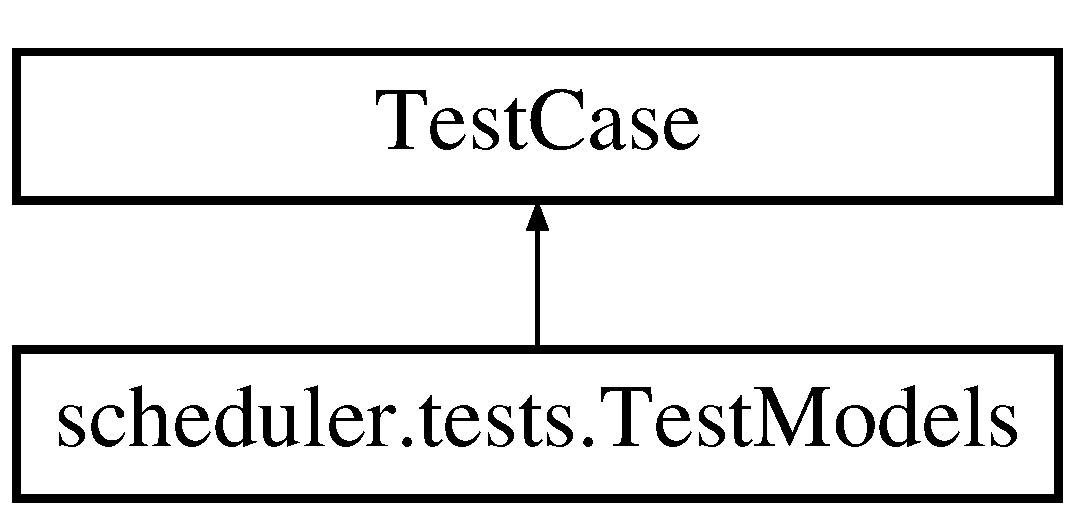
\includegraphics[height=2.000000cm]{classscheduler_1_1tests_1_1_test_models}
\end{center}
\end{figure}
\subsection*{Public Member Functions}
\begin{DoxyCompactItemize}
\item 
\hypertarget{classscheduler_1_1tests_1_1_test_models_af510ca5763450833e880baaf9ed65924}{def {\bfseries test\-\_\-named\-\_\-string\-\_\-representaion}}\label{classscheduler_1_1tests_1_1_test_models_af510ca5763450833e880baaf9ed65924}

\end{DoxyCompactItemize}


The documentation for this class was generated from the following file\-:\begin{DoxyCompactItemize}
\item 
/home/travis/build/\-Open-\/\-Source-\/\-Software-\/\-Development/class-\/scheduler/mysite/scheduler/tests.\-py\end{DoxyCompactItemize}

\hypertarget{classhibernate1_1_1_test_table}{\section{hibernate1.\-Test\-Table Class Reference}
\label{classhibernate1_1_1_test_table}\index{hibernate1.\-Test\-Table@{hibernate1.\-Test\-Table}}
}
Inheritance diagram for hibernate1.\-Test\-Table\-:\begin{figure}[H]
\begin{center}
\leavevmode
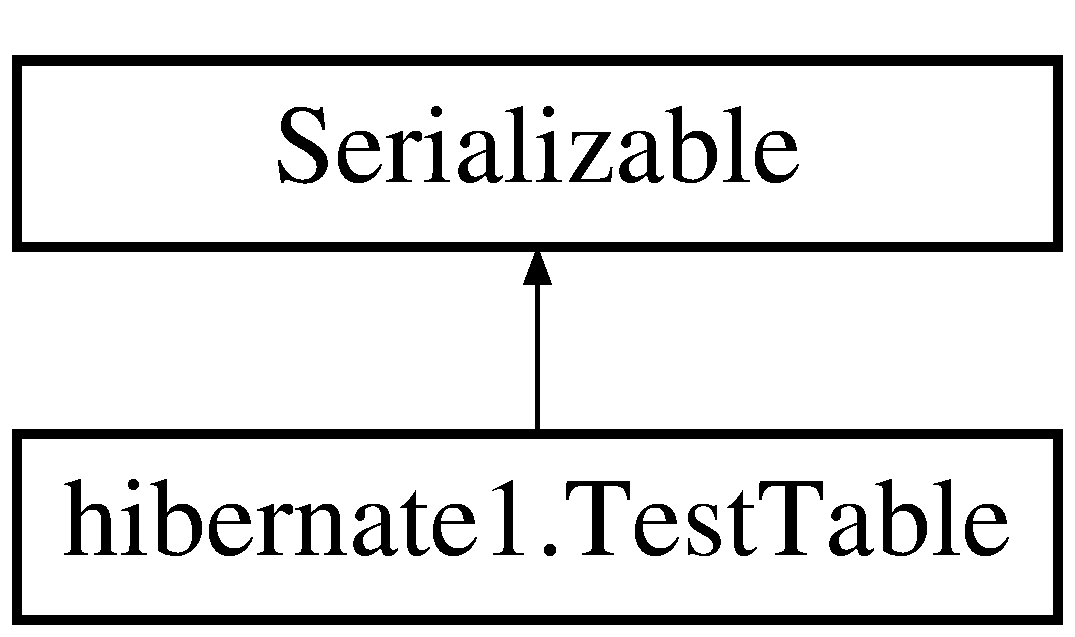
\includegraphics[height=2.000000cm]{classhibernate1_1_1_test_table}
\end{center}
\end{figure}
\subsection*{Public Member Functions}
\begin{DoxyCompactItemize}
\item 
\hypertarget{classhibernate1_1_1_test_table_af728065d4d2dd4f463434dd171be3a1b}{int {\bfseries get\-Id} ()}\label{classhibernate1_1_1_test_table_af728065d4d2dd4f463434dd171be3a1b}

\item 
\hypertarget{classhibernate1_1_1_test_table_ae440fd9fe93881027301fcc17ca2cdde}{void {\bfseries set\-Id} (int id)}\label{classhibernate1_1_1_test_table_ae440fd9fe93881027301fcc17ca2cdde}

\item 
\hypertarget{classhibernate1_1_1_test_table_a2d4f61cb8c64889bf633673c4985041d}{String {\bfseries get\-First\-Name} ()}\label{classhibernate1_1_1_test_table_a2d4f61cb8c64889bf633673c4985041d}

\item 
\hypertarget{classhibernate1_1_1_test_table_ab3bad26f58ae6ebe0312f2430c1cbe88}{void {\bfseries set\-First\-Name} (String first\-Name)}\label{classhibernate1_1_1_test_table_ab3bad26f58ae6ebe0312f2430c1cbe88}

\item 
\hypertarget{classhibernate1_1_1_test_table_a0ff3d75e7b9692928e5cfd72e3717928}{String {\bfseries get\-Last\-Name} ()}\label{classhibernate1_1_1_test_table_a0ff3d75e7b9692928e5cfd72e3717928}

\item 
\hypertarget{classhibernate1_1_1_test_table_a03e3e5395e928d366cd689869e8b8755}{void {\bfseries set\-Last\-Name} (String last\-Name)}\label{classhibernate1_1_1_test_table_a03e3e5395e928d366cd689869e8b8755}

\item 
\hypertarget{classhibernate1_1_1_test_table_a2ac7359341c8ba58f1468e942e46b0d1}{String {\bfseries get\-Division} ()}\label{classhibernate1_1_1_test_table_a2ac7359341c8ba58f1468e942e46b0d1}

\item 
\hypertarget{classhibernate1_1_1_test_table_a7630715bf4f2e4a8d64c41e569fd8571}{void {\bfseries set\-Division} (String division)}\label{classhibernate1_1_1_test_table_a7630715bf4f2e4a8d64c41e569fd8571}

\end{DoxyCompactItemize}


The documentation for this class was generated from the following file\-:\begin{DoxyCompactItemize}
\item 
/home/travis/build/\-Open-\/\-Source-\/\-Software-\/\-Development/class-\/scheduler/hibernate\-Setup/src/hibernate1/Test\-Table.\-java\end{DoxyCompactItemize}

\hypertarget{classosd_1_1considerations_1_1_user_consideration}{\section{osd.\-considerations.\-User\-Consideration Class Reference}
\label{classosd_1_1considerations_1_1_user_consideration}\index{osd.\-considerations.\-User\-Consideration@{osd.\-considerations.\-User\-Consideration}}
}
Inheritance diagram for osd.\-considerations.\-User\-Consideration\-:\begin{figure}[H]
\begin{center}
\leavevmode
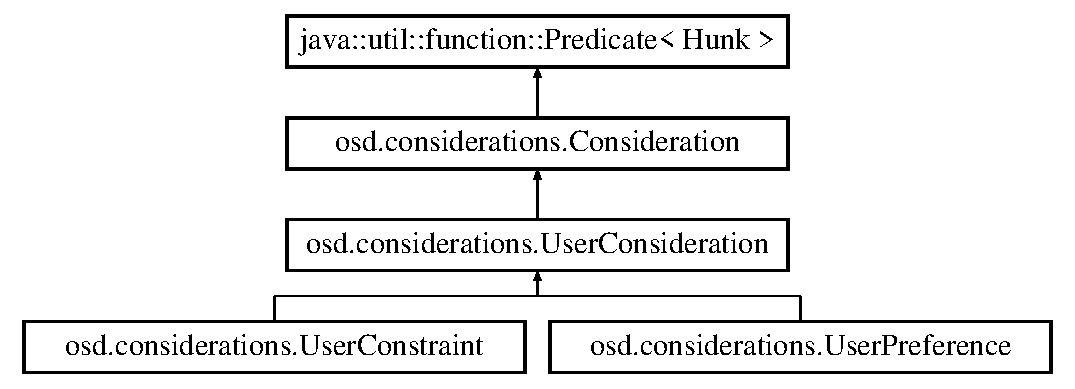
\includegraphics[height=4.000000cm]{classosd_1_1considerations_1_1_user_consideration}
\end{center}
\end{figure}
\subsection*{Classes}
\begin{DoxyCompactItemize}
\item 
enum {\bfseries Match}
\end{DoxyCompactItemize}


\subsection{Detailed Description}
Abstract base class for user preferences and constraints. User preferences and constraints are both defined as pairs of scheduling elements. For example, a constraint indicating Professor Brown can't teach block 7\-A would have one of its members be Professor Brown and the other be block 7\-A. 

What exactly this pair {\itshape means} is up to the specific implementation, however. The purpose of this class is to provide an easy way to check how many members match, not to interpret that result.

\begin{DoxySeeAlso}{See Also}
\#get\-Match(\-Hunk) 
\end{DoxySeeAlso}


The documentation for this class was generated from the following file\-:\begin{DoxyCompactItemize}
\item 
/home/travis/build/\-Open-\/\-Source-\/\-Software-\/\-Development/class-\/scheduler/java/src/main/java/osd/considerations/User\-Consideration.\-java\end{DoxyCompactItemize}

\hypertarget{classosd_1_1considerations_1_1_user_consideration_module}{\section{osd.\-considerations.\-User\-Consideration\-Module Class Reference}
\label{classosd_1_1considerations_1_1_user_consideration_module}\index{osd.\-considerations.\-User\-Consideration\-Module@{osd.\-considerations.\-User\-Consideration\-Module}}
}


The documentation for this class was generated from the following file\-:\begin{DoxyCompactItemize}
\item 
/home/travis/build/\-Open-\/\-Source-\/\-Software-\/\-Development/class-\/scheduler/java/src/main/java/osd/considerations/User\-Consideration\-Module.\-java\end{DoxyCompactItemize}

\hypertarget{classosd_1_1considerations_1_1_user_constraint}{\section{osd.\-considerations.\-User\-Constraint Class Reference}
\label{classosd_1_1considerations_1_1_user_constraint}\index{osd.\-considerations.\-User\-Constraint@{osd.\-considerations.\-User\-Constraint}}
}
Inheritance diagram for osd.\-considerations.\-User\-Constraint\-:\begin{figure}[H]
\begin{center}
\leavevmode
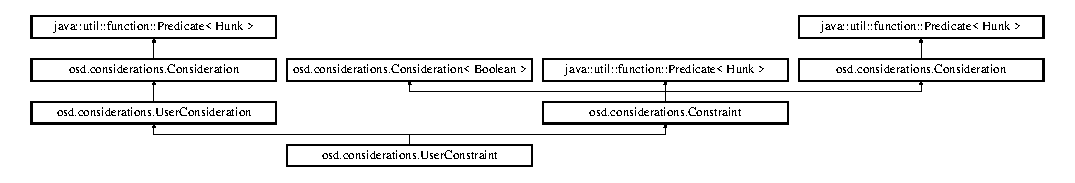
\includegraphics[height=2.014389cm]{classosd_1_1considerations_1_1_user_constraint}
\end{center}
\end{figure}
\subsection*{Public Member Functions}
\begin{DoxyCompactItemize}
\item 
boolean \hyperlink{classosd_1_1considerations_1_1_user_constraint_a9378d413848106a42ede0782730c0408}{test} (final \hyperlink{classosd_1_1output_1_1_hunk}{Hunk} hunk)
\end{DoxyCompactItemize}
\subsection*{Additional Inherited Members}


\subsection{Detailed Description}
User constraints use their element pairs as white-\/ or blacklists. See  \hyperlink{classosd_1_1considerations_1_1_user_consideration}{User\-Consideration} the parent class documentation\} for what an \char`\"{}element pair\char`\"{} is. Blacklist constraints are satisfied if at least one member doesn't match. Whitelist constraints are satisfied if either both members match or neither does. 

\subsection{Member Function Documentation}
\hypertarget{classosd_1_1considerations_1_1_user_constraint_a9378d413848106a42ede0782730c0408}{\index{osd\-::considerations\-::\-User\-Constraint@{osd\-::considerations\-::\-User\-Constraint}!test@{test}}
\index{test@{test}!osd::considerations::UserConstraint@{osd\-::considerations\-::\-User\-Constraint}}
\subsubsection[{test}]{\setlength{\rightskip}{0pt plus 5cm}boolean osd.\-considerations.\-User\-Constraint.\-test (
\begin{DoxyParamCaption}
\item[{final {\bf Hunk}}]{hunk}
\end{DoxyParamCaption}
)\hspace{0.3cm}{\ttfamily [inline]}}}\label{classosd_1_1considerations_1_1_user_constraint_a9378d413848106a42ede0782730c0408}
Determines whether some hunk satisfies this consideration. If the consideration is indeterminate because the hunk contains
\begin{DoxyCode}
null 
\end{DoxyCode}
 s, the result must be
\begin{DoxyCode}
\textcolor{keyword}{true} 
\end{DoxyCode}
 . 
\begin{DoxyParams}{Parameters}
{\em hunk} & a hunk \\
\hline
\end{DoxyParams}
\begin{DoxyReturn}{Returns}
true if the hunk passes or is indeterminate, false if it fails 
\end{DoxyReturn}


Implements \hyperlink{interfaceosd_1_1considerations_1_1_constraint_a50c53a0c89a4cfb8b58deae081ca3787}{osd.\-considerations.\-Constraint}.



The documentation for this class was generated from the following file\-:\begin{DoxyCompactItemize}
\item 
/home/travis/build/\-Open-\/\-Source-\/\-Software-\/\-Development/class-\/scheduler/java/src/main/java/osd/considerations/User\-Constraint.\-java\end{DoxyCompactItemize}

\hypertarget{classscheduler_1_1models_1_1_user_constraint}{\section{scheduler.\-models.\-User\-Constraint Class Reference}
\label{classscheduler_1_1models_1_1_user_constraint}\index{scheduler.\-models.\-User\-Constraint@{scheduler.\-models.\-User\-Constraint}}
}
Inheritance diagram for scheduler.\-models.\-User\-Constraint\-:\begin{figure}[H]
\begin{center}
\leavevmode
\includegraphics[height=3.000000cm]{classscheduler_1_1models_1_1_user_constraint}
\end{center}
\end{figure}
\subsection*{Public Member Functions}
\begin{DoxyCompactItemize}
\item 
\hypertarget{classscheduler_1_1models_1_1_user_constraint_a69ca598611d4eb869e25db7dd9cd3659}{def {\bfseries describe}}\label{classscheduler_1_1models_1_1_user_constraint_a69ca598611d4eb869e25db7dd9cd3659}

\end{DoxyCompactItemize}
\subsection*{Static Public Attributes}
\begin{DoxyCompactItemize}
\item 
\hypertarget{classscheduler_1_1models_1_1_user_constraint_a120a4f7219a677bc9940a486ec0fff4f}{tuple {\bfseries is\-\_\-blacklist} = models.\-Boolean\-Field()}\label{classscheduler_1_1models_1_1_user_constraint_a120a4f7219a677bc9940a486ec0fff4f}

\end{DoxyCompactItemize}


\subsection{Detailed Description}
\begin{DoxyVerb}    Table: UserConstraint
    Primary Key: Autogenerated ID
    Columns:
        is_blacklist: Bool
\end{DoxyVerb}
 

The documentation for this class was generated from the following file\-:\begin{DoxyCompactItemize}
\item 
/home/travis/build/\-Open-\/\-Source-\/\-Software-\/\-Development/class-\/scheduler/mysite/scheduler/models.\-py\end{DoxyCompactItemize}

\hypertarget{classosd_1_1database_1_1_user_constraint_factory}{\section{osd.\-database.\-User\-Constraint\-Factory Class Reference}
\label{classosd_1_1database_1_1_user_constraint_factory}\index{osd.\-database.\-User\-Constraint\-Factory@{osd.\-database.\-User\-Constraint\-Factory}}
}
Inheritance diagram for osd.\-database.\-User\-Constraint\-Factory\-:\begin{figure}[H]
\begin{center}
\leavevmode
\includegraphics[height=2.000000cm]{classosd_1_1database_1_1_user_constraint_factory}
\end{center}
\end{figure}
\subsection*{Public Member Functions}
\begin{DoxyCompactItemize}
\item 
\hypertarget{classosd_1_1database_1_1_user_constraint_factory_a18370b0280bac769da6e4498b3a22a8d}{\hyperlink{classosd_1_1considerations_1_1_user_constraint}{User\-Constraint} {\bfseries create} (final \hyperlink{classosd_1_1database_1_1_user_constraint_record}{User\-Constraint\-Record} record)}\label{classosd_1_1database_1_1_user_constraint_factory_a18370b0280bac769da6e4498b3a22a8d}

\end{DoxyCompactItemize}


The documentation for this class was generated from the following file\-:\begin{DoxyCompactItemize}
\item 
/home/travis/build/\-Open-\/\-Source-\/\-Software-\/\-Development/class-\/scheduler/java/src/main/java/osd/database/User\-Constraint\-Factory.\-java\end{DoxyCompactItemize}

\hypertarget{classosd_1_1database_1_1_user_constraint_record}{\section{osd.\-database.\-User\-Constraint\-Record Class Reference}
\label{classosd_1_1database_1_1_user_constraint_record}\index{osd.\-database.\-User\-Constraint\-Record@{osd.\-database.\-User\-Constraint\-Record}}
}


The documentation for this class was generated from the following file\-:\begin{DoxyCompactItemize}
\item 
/home/travis/build/\-Open-\/\-Source-\/\-Software-\/\-Development/class-\/scheduler/java/src/main/java/osd/database/User\-Constraint\-Record.\-java\end{DoxyCompactItemize}

\hypertarget{classosd_1_1considerations_1_1_user_preference}{\section{osd.\-considerations.\-User\-Preference Class Reference}
\label{classosd_1_1considerations_1_1_user_preference}\index{osd.\-considerations.\-User\-Preference@{osd.\-considerations.\-User\-Preference}}
}
Inheritance diagram for osd.\-considerations.\-User\-Preference\-:\begin{figure}[H]
\begin{center}
\leavevmode
\includegraphics[height=2.755228cm]{classosd_1_1considerations_1_1_user_preference}
\end{center}
\end{figure}
\subsection*{Public Member Functions}
\begin{DoxyCompactItemize}
\item 
\hypertarget{classosd_1_1considerations_1_1_user_preference_a486463a2349d6884906a5cc6ccbfb570}{int {\bfseries worth} ()}\label{classosd_1_1considerations_1_1_user_preference_a486463a2349d6884906a5cc6ccbfb570}

\item 
\hypertarget{classosd_1_1considerations_1_1_user_preference_ad30f1b5c2001ed4f2b5719f8ae62121b}{boolean {\bfseries test} (final \hyperlink{classosd_1_1output_1_1_hunk}{Hunk} hunk)}\label{classosd_1_1considerations_1_1_user_preference_ad30f1b5c2001ed4f2b5719f8ae62121b}

\end{DoxyCompactItemize}


The documentation for this class was generated from the following file\-:\begin{DoxyCompactItemize}
\item 
/home/travis/build/\-Open-\/\-Source-\/\-Software-\/\-Development/class-\/scheduler/java/src/main/java/osd/considerations/User\-Preference.\-java\end{DoxyCompactItemize}

\hypertarget{classscheduler_1_1models_1_1_user_preference}{\section{scheduler.\-models.\-User\-Preference Class Reference}
\label{classscheduler_1_1models_1_1_user_preference}\index{scheduler.\-models.\-User\-Preference@{scheduler.\-models.\-User\-Preference}}
}


T\-O\-D\-O\-: Documentation.  


Inheritance diagram for scheduler.\-models.\-User\-Preference\-:\begin{figure}[H]
\begin{center}
\leavevmode
\includegraphics[height=3.000000cm]{classscheduler_1_1models_1_1_user_preference}
\end{center}
\end{figure}
\subsection*{Public Member Functions}
\begin{DoxyCompactItemize}
\item 
\hypertarget{classscheduler_1_1models_1_1_user_preference_a9f811ec38d568d99837e79b2b0699da6}{def \hyperlink{classscheduler_1_1models_1_1_user_preference_a9f811ec38d568d99837e79b2b0699da6}{describe}}\label{classscheduler_1_1models_1_1_user_preference_a9f811ec38d568d99837e79b2b0699da6}

\begin{DoxyCompactList}\small\item\em T\-O\-D\-O\-: Documentation. \end{DoxyCompactList}\end{DoxyCompactItemize}
\subsection*{Static Public Attributes}
\begin{DoxyCompactItemize}
\item 
\hypertarget{classscheduler_1_1models_1_1_user_preference_aefe583851d963dac6a85e6f8badfbffa}{tuple \hyperlink{classscheduler_1_1models_1_1_user_preference_aefe583851d963dac6a85e6f8badfbffa}{score} = models.\-Integer\-Field()}\label{classscheduler_1_1models_1_1_user_preference_aefe583851d963dac6a85e6f8badfbffa}

\begin{DoxyCompactList}\small\item\em T\-O\-D\-O\-: Documentation. \end{DoxyCompactList}\end{DoxyCompactItemize}


\subsection{Detailed Description}
T\-O\-D\-O\-: Documentation. 

The documentation for this class was generated from the following file\-:\begin{DoxyCompactItemize}
\item 
/home/travis/build/\-Open-\/\-Source-\/\-Software-\/\-Development/class-\/scheduler/mysite/scheduler/models.\-py\end{DoxyCompactItemize}

\hypertarget{classosd_1_1database_1_1_user_preference_factory}{\section{osd.\-database.\-User\-Preference\-Factory Class Reference}
\label{classosd_1_1database_1_1_user_preference_factory}\index{osd.\-database.\-User\-Preference\-Factory@{osd.\-database.\-User\-Preference\-Factory}}
}
Inheritance diagram for osd.\-database.\-User\-Preference\-Factory\-:\begin{figure}[H]
\begin{center}
\leavevmode
\includegraphics[height=2.000000cm]{classosd_1_1database_1_1_user_preference_factory}
\end{center}
\end{figure}
\subsection*{Public Member Functions}
\begin{DoxyCompactItemize}
\item 
\hypertarget{classosd_1_1database_1_1_user_preference_factory_ab3a50656c26560d1bca36f320aa2e917}{\hyperlink{classosd_1_1considerations_1_1_user_preference}{User\-Preference} {\bfseries create} (final \hyperlink{classosd_1_1database_1_1_user_preference_record}{User\-Preference\-Record} record)}\label{classosd_1_1database_1_1_user_preference_factory_ab3a50656c26560d1bca36f320aa2e917}

\end{DoxyCompactItemize}


The documentation for this class was generated from the following file\-:\begin{DoxyCompactItemize}
\item 
/home/travis/build/\-Open-\/\-Source-\/\-Software-\/\-Development/class-\/scheduler/java/src/main/java/osd/database/User\-Preference\-Factory.\-java\end{DoxyCompactItemize}

\hypertarget{classscheduler_1_1models_1_1_user_preference_or_constraint}{\section{scheduler.\-models.\-User\-Preference\-Or\-Constraint Class Reference}
\label{classscheduler_1_1models_1_1_user_preference_or_constraint}\index{scheduler.\-models.\-User\-Preference\-Or\-Constraint@{scheduler.\-models.\-User\-Preference\-Or\-Constraint}}
}


T\-O\-D\-O\-: Documentation.  


Inheritance diagram for scheduler.\-models.\-User\-Preference\-Or\-Constraint\-:\begin{figure}[H]
\begin{center}
\leavevmode
\includegraphics[height=2.947368cm]{classscheduler_1_1models_1_1_user_preference_or_constraint}
\end{center}
\end{figure}
\subsection*{Classes}
\begin{DoxyCompactItemize}
\item 
class \hyperlink{classscheduler_1_1models_1_1_user_preference_or_constraint_1_1_meta}{Meta}
\end{DoxyCompactItemize}
\subsection*{Public Member Functions}
\begin{DoxyCompactItemize}
\item 
\hypertarget{classscheduler_1_1models_1_1_user_preference_or_constraint_a1b04b83430b49ef79badd95682e6cf4e}{def \hyperlink{classscheduler_1_1models_1_1_user_preference_or_constraint_a1b04b83430b49ef79badd95682e6cf4e}{\-\_\-\-\_\-str\-\_\-\-\_\-}}\label{classscheduler_1_1models_1_1_user_preference_or_constraint_a1b04b83430b49ef79badd95682e6cf4e}

\begin{DoxyCompactList}\small\item\em T\-O\-D\-O\-: Documentation. \end{DoxyCompactList}\item 
\hypertarget{classscheduler_1_1models_1_1_user_preference_or_constraint_a8198615fa62dee4ea1cb89fe6ab834e0}{def \hyperlink{classscheduler_1_1models_1_1_user_preference_or_constraint_a8198615fa62dee4ea1cb89fe6ab834e0}{describe}}\label{classscheduler_1_1models_1_1_user_preference_or_constraint_a8198615fa62dee4ea1cb89fe6ab834e0}

\begin{DoxyCompactList}\small\item\em T\-O\-D\-O\-: Documentation. \end{DoxyCompactList}\end{DoxyCompactItemize}
\subsection*{Static Public Attributes}
\begin{DoxyCompactItemize}
\item 
\hypertarget{classscheduler_1_1models_1_1_user_preference_or_constraint_a0455877d277a31c0561935c7074b664b}{tuple \hyperlink{classscheduler_1_1models_1_1_user_preference_or_constraint_a0455877d277a31c0561935c7074b664b}{left\-\_\-argument\-\_\-type} = models.\-Foreign\-Key(Content\-Type, on\-\_\-delete=models.\-C\-A\-S\-C\-A\-D\-E, related\-\_\-name=\char`\"{}+\char`\"{})}\label{classscheduler_1_1models_1_1_user_preference_or_constraint_a0455877d277a31c0561935c7074b664b}

\begin{DoxyCompactList}\small\item\em T\-O\-D\-O\-: Documentation. \end{DoxyCompactList}\item 
\hypertarget{classscheduler_1_1models_1_1_user_preference_or_constraint_aa1b1f271f6f1f18d5e99996db4840337}{tuple \hyperlink{classscheduler_1_1models_1_1_user_preference_or_constraint_aa1b1f271f6f1f18d5e99996db4840337}{left\-\_\-argument\-\_\-id} = models.\-Positive\-Integer\-Field()}\label{classscheduler_1_1models_1_1_user_preference_or_constraint_aa1b1f271f6f1f18d5e99996db4840337}

\begin{DoxyCompactList}\small\item\em T\-O\-D\-O\-: Documentation. \end{DoxyCompactList}\item 
\hypertarget{classscheduler_1_1models_1_1_user_preference_or_constraint_a1880c90f057ecd54a9a484faa30e3df5}{tuple \hyperlink{classscheduler_1_1models_1_1_user_preference_or_constraint_a1880c90f057ecd54a9a484faa30e3df5}{left\-\_\-argument\-\_\-object} = Generic\-Foreign\-Key('\hyperlink{classscheduler_1_1models_1_1_user_preference_or_constraint_a0455877d277a31c0561935c7074b664b}{left\-\_\-argument\-\_\-type}', '\hyperlink{classscheduler_1_1models_1_1_user_preference_or_constraint_aa1b1f271f6f1f18d5e99996db4840337}{left\-\_\-argument\-\_\-id}')}\label{classscheduler_1_1models_1_1_user_preference_or_constraint_a1880c90f057ecd54a9a484faa30e3df5}

\begin{DoxyCompactList}\small\item\em T\-O\-D\-O\-: Documentation. \end{DoxyCompactList}\item 
\hypertarget{classscheduler_1_1models_1_1_user_preference_or_constraint_a30dcc18f79528b7860691bced63d3426}{tuple \hyperlink{classscheduler_1_1models_1_1_user_preference_or_constraint_a30dcc18f79528b7860691bced63d3426}{right\-\_\-argument\-\_\-type} = models.\-Foreign\-Key(Content\-Type, on\-\_\-delete=models.\-C\-A\-S\-C\-A\-D\-E, related\-\_\-name=\char`\"{}+\char`\"{})}\label{classscheduler_1_1models_1_1_user_preference_or_constraint_a30dcc18f79528b7860691bced63d3426}

\begin{DoxyCompactList}\small\item\em T\-O\-D\-O\-: Documentation. \end{DoxyCompactList}\item 
\hypertarget{classscheduler_1_1models_1_1_user_preference_or_constraint_adbb69d170fd984fe2ec36e340cdf3533}{tuple \hyperlink{classscheduler_1_1models_1_1_user_preference_or_constraint_adbb69d170fd984fe2ec36e340cdf3533}{right\-\_\-argument\-\_\-id} = models.\-Positive\-Integer\-Field()}\label{classscheduler_1_1models_1_1_user_preference_or_constraint_adbb69d170fd984fe2ec36e340cdf3533}

\begin{DoxyCompactList}\small\item\em T\-O\-D\-O\-: Documentation. \end{DoxyCompactList}\item 
\hypertarget{classscheduler_1_1models_1_1_user_preference_or_constraint_a3a80b4294939af457c24a9377bc43239}{tuple \hyperlink{classscheduler_1_1models_1_1_user_preference_or_constraint_a3a80b4294939af457c24a9377bc43239}{right\-\_\-argument\-\_\-object} = Generic\-Foreign\-Key('\hyperlink{classscheduler_1_1models_1_1_user_preference_or_constraint_a30dcc18f79528b7860691bced63d3426}{right\-\_\-argument\-\_\-type}', '\hyperlink{classscheduler_1_1models_1_1_user_preference_or_constraint_adbb69d170fd984fe2ec36e340cdf3533}{right\-\_\-argument\-\_\-id}')}\label{classscheduler_1_1models_1_1_user_preference_or_constraint_a3a80b4294939af457c24a9377bc43239}

\begin{DoxyCompactList}\small\item\em T\-O\-D\-O\-: Documentation. \end{DoxyCompactList}\end{DoxyCompactItemize}


\subsection{Detailed Description}
T\-O\-D\-O\-: Documentation. 

The documentation for this class was generated from the following file\-:\begin{DoxyCompactItemize}
\item 
/home/travis/build/\-Open-\/\-Source-\/\-Software-\/\-Development/class-\/scheduler/mysite/scheduler/models.\-py\end{DoxyCompactItemize}

\hypertarget{classosd_1_1database_1_1_user_preference_record}{\section{osd.\-database.\-User\-Preference\-Record Class Reference}
\label{classosd_1_1database_1_1_user_preference_record}\index{osd.\-database.\-User\-Preference\-Record@{osd.\-database.\-User\-Preference\-Record}}
}


The documentation for this class was generated from the following file\-:\begin{DoxyCompactItemize}
\item 
/home/travis/build/\-Open-\/\-Source-\/\-Software-\/\-Development/class-\/scheduler/java/src/main/java/osd/database/User\-Preference\-Record.\-java\end{DoxyCompactItemize}

\hypertarget{interfaceosd_1_1considerations_1_1_constraint_1_1_whitelist}{\section{osd.\-considerations.\-Constraint.\-Whitelist Interface Reference}
\label{interfaceosd_1_1considerations_1_1_constraint_1_1_whitelist}\index{osd.\-considerations.\-Constraint.\-Whitelist@{osd.\-considerations.\-Constraint.\-Whitelist}}
}
Inheritance diagram for osd.\-considerations.\-Constraint.\-Whitelist\-:\begin{figure}[H]
\begin{center}
\leavevmode
\includegraphics[height=2.685851cm]{interfaceosd_1_1considerations_1_1_constraint_1_1_whitelist}
\end{center}
\end{figure}
\subsection*{Public Member Functions}
\begin{DoxyCompactItemize}
\item 
\hypertarget{interfaceosd_1_1considerations_1_1_constraint_1_1_whitelist_a42fe7cf245fe854652d98af0f7f7d3e7}{default Type {\bfseries get\-Type} ()}\label{interfaceosd_1_1considerations_1_1_constraint_1_1_whitelist_a42fe7cf245fe854652d98af0f7f7d3e7}

\end{DoxyCompactItemize}
\subsection*{Additional Inherited Members}


The documentation for this interface was generated from the following file\-:\begin{DoxyCompactItemize}
\item 
/home/travis/build/\-Open-\/\-Source-\/\-Software-\/\-Development/class-\/scheduler/src/main/java/osd/considerations/Constraint.\-java\end{DoxyCompactItemize}

%--- End generated contents ---

% Index
\newpage
\phantomsection
\addcontentsline{toc}{chapter}{Index}
\printindex

\end{document}
